\documentclass{article}
\usepackage{ctex}
\usepackage[a4paper,left=10mm,right=10mm,top=15mm,bottom=15mm]{geometry}
\usepackage{graphicx}
\usepackage{amsfonts,amssymb}
\usepackage{amsmath}
\usepackage{biblatex}
\usepackage{hyperref}
\usepackage{color}
\usepackage{titlesec}
\usepackage{titletoc}
\usepackage{listings}

\title{代码大全笔记}
\author{张谦}
\date{\today}
\begin{document}
\maketitle
\tableofcontents
\newpage

\section{欢迎进入软件构件的世界}
\subsection{什么是软件构建}
如下图所示,构建活动主要是编码与调试,但也涉及详细设计、规划构建、单元测试、集成、集成测试
等其他活动。
\begin{figure}[ht]
    \centering
    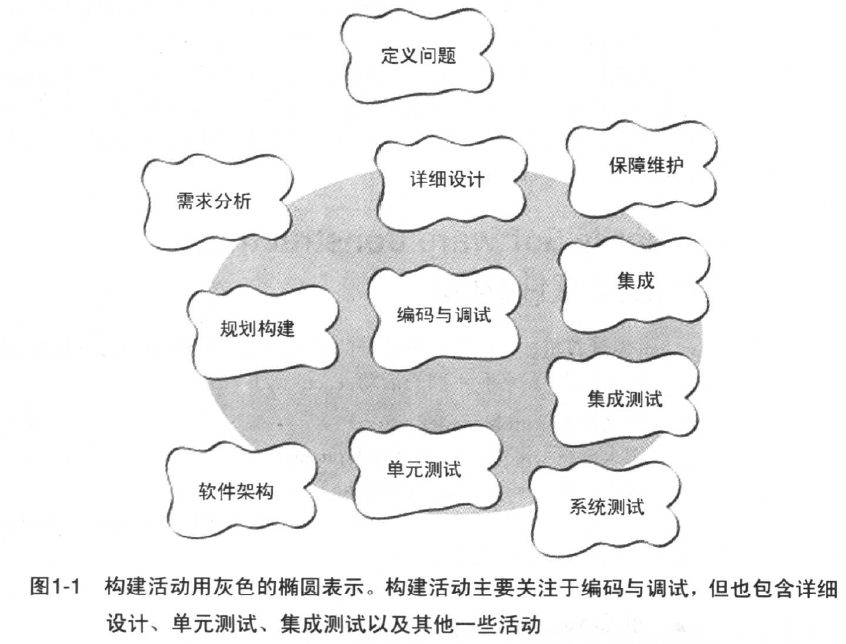
\includegraphics[width=10cm]{figure1.png}
\end{figure}

\par
构建活动包含如下具体任务:
\begin{itemize}
    \item 验证有关的基础工作已经完成,保证构建活动可以顺利进行;
    \item 确定如何测试所写的代码;
    \item 设计并编写类和子程序;
    \item 创建并命名变量和具名常量;
    \item 选择控制结构,组织语句块;
    \item 对代码进行单元测试和集成测试,并排除其中的错误;
    \item 评审开发团队其他成员的底层设计和代码,并让他们评审你的工作;
    \item 优化代码,仔细进行代码的格式化和注释;
    \item 将单独开发的多个组件集成为一体;
    \item 调整代码,让它更快、更省资源。
\end{itemize}

\subsection{构建为什么重要}
\begin{itemize}
    \item 构建活动是软件开发的主要组成部分;
    \item 构建活动是软件开发中的核心活动;
    \item 将主要精力集中于构建活动,可以大大提高程序员生产率;
    \item 构建活动的产物,源代码,往往是对软件的唯一精确描述;
    \item 构建活动是唯一一项确保完成的工作。
\end{itemize}

\section{用隐喻理解软件开发}
隐喻是启示而不是算法,可以将软件开发过程与其他熟悉的活动联系在一起,帮助更好地理解开发过程。
相比其他隐喻,例如写作、种植和养殖等,通过将软件的构建过程,比作房屋的建设过程,能够更好地
理解软件构建的各个阶段。
\subsection{建造隐喻}
\par
(1)问题定义(problem definition):决定准备建一个什么类型的房子;
\par
(2)架构设计(architectural design):和某个建筑师探讨总体设计,并得到批准;
\par
(3)详细设计:画出详细的蓝图,雇一个承包人;
\par
(4)软件构建(construction):准备好建造地点,打好地基,搭建房屋框架,砌好边墙,盖好房顶,
通好水、电、煤气等;
\par
(5)软件优化:在房子大部分完成后,庭院设计师、油漆匠和装修工还要把新盖的房子以及里面的家什
美化一番;
\par
(6)评审和审查(reviews,inspections):在整个过程中,还会有各种监察人员来检查工地、地基、
框架、布线以及其他需要检查的地方。

\subsection{已有组件}
当开发软件时,会大量使用高级语言所提供的功能,而不会自己去编写操作系统层次的代码;
自己编写那些能买得到的现成程序库是没有意义的,例如一些容器类、科学计算函数、用户界面组件、
数据库访问组件等。在建造房子的时候,你也不会去试着建造那些能买得到的东西,例如洗衣机、
冰箱、餐桌等。

\subsection{定制组件}
如果想建造一间拥有一流家具的高档住宅,可能就需要定制的橱柜,以及和橱柜搭配的洗碗机和冰箱等。
在软件开发中也有这种订制的情况,例如想要开发一款一流的软件产品,可能会自己编写科学计算函数,
以便获得更快的速度和更高的精度。

\subsection{防止过度计划}
适当的多层次规划对于建造房屋和构建软件都是有好处的,如果按错误的顺序构建软件,那么编码、测试和
调试都会很难。精心计划,并不是事无巨细的计划或过度计划,例如你可以把房屋的结构性支撑规划清楚,
在日后再决定是用木地板还是瓷砖地板,墙面漆成什么颜色等。

\subsection{不同软件项目}
建筑业中,盖一间仓库或工具房,或是一座医院或核反应站,在规划、设计和质量保证方面所需达到的程度
是不一样的,所用的方法也不相同。同理,在软件开发中,通常只需要用灵活的、轻量级的方法,但有时
你就必须用严格的、重量级的开发方法,以达到所需的安全性目标或其他目标。
另外,还需要特别关注工作时间,在建造帝国大厦时,每辆运料车运输时都留有15分钟的余地,如果
某辆车没能在指定的时间到位,则整个工期就会延误。对于超大型的软件项目,就需要比一般规模的项目
有更高级的规划设计,如果需要创造在经济规模上可以匹敌帝国大厦的庞大软件项目,那么与之相当
水准的技术与管理控制也是必需的。

\section{构建前期准备}
\subsection{前期准备的重要性}
准备工作的中心目标就是降低风险,软件开发中最常见的项目风险是糟糕的需求分析和糟糕的项目计划,
因此准备工作就倾向于集中改进需求分析和项目规划。
高质量的实践方法在项目的初期、中期和末期都强调质量:
\par
(1)如果在项目末期强调质量,那么你会强调系统测试;但是测试只是完整的质量保证策略的一部分,
而且不是最有影响的部分;
\par
(2)如果在项目中期强调质量,那么你会强调构建实践;
\par
(3)如果在项目开始阶段强调质量,那么你就会计划、要求并设计一个高质量的产品;例如你用为吉利车
做的设计来开始整个生产过程,尽管你可以想尽办法来测试,它也绝对不会变成奔驰;也许你能造出最好
的吉利车,但是如果你想要的是奔驰,那么你就得从头开始做设计。

\subsection{序列式开发和迭代式开发选择}
绝大多数的项目都不会完全使用序列式开发法或完全使用迭代式开发法。预先详细说明100\%的需求
和设计是不切实际的,不过对绝大多数项目来说,尽早把那些最关键的需求要素和架构要素确定下来,
时很有价值。
\par
可能因为下列原因选择一个更加迭代的方法:
\begin{itemize}
    \item 需求并没有被理解透彻,或者出于其他理由你认为它是不稳定的;
    \item 设计很复杂,或者有挑战性,或者两者兼具;
    \item 开发团队对于这一应用领域不熟悉;
    \item 项目包含许多风险;
    \item “长期可预测性”不重要;
    \item 后期改变需求、设计和编码的代价很可能比较低。
\end{itemize}
相反的,你可能需要选择一个更加序列的方法。

\subsection{问题定义的先决条件}
在开始构建之前,首先要满足的一项先决条件是,对这个系统要解决的问题做出清楚的陈述。
问题定义只定义了问题是什么,而不涉及任何可能的解决方案。它是一个很简单的陈述,并且听起来
应该像个问题。例如“我们跟不上客户的订单了”听起来就像个问题,而且确实是一个很好的问题
定义;而“我们需要优化数据自动采集系统,使之跟上客户的订单”,这种就是糟糕的问题定义,
它听起来不像问题,而像解决方案。另外,问题定义应该用客户的语言来书写,而且应该从客户的
角度来描述问题。

\subsection{需求的先决条件}
“需求”详细描述软件系统应该做什么,这是达成解决方案的第一步。需求明确有如下好处:
\begin{itemize}
    \item 用户可以自行评审,并进行核准;否则程序员就常常会在编程期间自行决定需求;
    \item 有助于避免争论,如果你和另外一个程序员有分歧,可以查看书面的需求,已解决分歧;
    \item 有助于减少开始编程开发之后的系统变更的情况;
    \item 充分详尽地描述需求,是项目成功的关键,它甚至很可能比有效的构建技术更重要。
\end{itemize}

\par
在构建期间处理需求变更,有以下一些可以采用的方式:
\begin{itemize}
    \item 评估需求质量,如果需求不够好,则停止工作,退回去,先做好后再继续前进;
    \item 确保每一个人都知道需求变更的代价;
    \item 建立一套变更控制程序;
    \item 使用能适应变更的开发方法;
    \item 放弃这个项目;
    \item 注意项目的商业案例,注重商业价值。
\end{itemize}

\subsection{架构的先决条件}
软件架构是软件设计的高层部分,是用于支持更细节设计的框架。架构的质量决定了系统的“概念完整性”,
继而决定了系统的最终质量。一个经过慎重考虑的架构,为“从顶层到底层维护系统的概念完整性”,提供
了必备的结构和体系,它为程序员提供了指引,其细节程度与程序员的技能和手边的工作相配;它将
工作分为几个部分,使多个开发者或多个开发团队可以独立工作。
\par
架构的典型组成部分:
\par
(1)程序组织:
\begin{itemize}
    \item 系统架构首先要以概括的形式对有关系统做一个综述;
    \item 在架构中,应该能发现对那些曾经考虑过的,最终组织结构的,替代方案的记叙;
    找到之所以选用最终的组织结构,而不是其他替代方案的理由;
    \item 架构应该定义程序的主要构造块,根据程序规模的不同,各个构造块可能是单个类,也可能是由
    许多类组成的一个子系统;
    \item 应该明确定义各个构造块的责任,每个构造块应该负责某一个区域的事情,并且对其他构造块负责的
区域知道得越少越好,将设计的信息局限在各个构造块之内;
    \item 应该明确定义每个构造块的通信规则,对于每个构造块,架构应该描述它能直接使用那些构造块,能
间接使用哪些构造块,不能使用哪些构造块。
\end{itemize}

\par
(2)主要的类:
\begin{itemize}
    \item 架构应该详细定义所用的主要的类,应该指出每个主要的类的责任,以及该类如何与其他类交互;
    它应该包含对类的继承体系、状态转换、对象持久化等的描述;如果系统足够大,它应该描述如何将
    这类组织成一个个子系统;
    \item 架构应该记述曾经考虑过的其他类设计方案,并给出选用当前方案的理由;架构无需详细说明
    系统中的每一个类,利用80/20法则:对那些构成系统80\%的行为的20\%的类进行详细说明。
\end{itemize}

\par
(3)数据设计:
\begin{itemize}
    \item 架构应该描述所用到的主要文件和数据表的设计。它应该描述曾经考虑过的其他方案,并说明
    选择当前方案的原因。如果应用程序要维护一个客户ID的列表,而架构师决定使用顺序访问的列表来
    表示该ID的列表,那么文档就应该解释为什么顺序访问的列表比随机访问的列表、堆栈、散列表要好。
    在构建期间,这些信息让你能洞察架构师的思想;在维护阶段,这种洞察力是无价之宝。离开它,你就像
    看一部没有字幕的外语片;
    \item 数据通常只应该由一个子系统或一个类直接访问;例外的情况就是通过访问器类或访问器子程序,
    以受控且抽象的方式来访问数据;
    \item 架构应该详细定义所用数据库的高层组织结构和内容;架构应该解释为什么单个数据库比多个数据库
    要好,反之亦然。需要解释为什么不用平坦的文件,而要用数据库,指出与其他访问同一数据的程序的
    可能交互方式,说明创建哪些数据视图等等。
\end{itemize}

\par
(4)业务规则:
\par
如果架构依赖于特定的业务规则,那么它就应该详细描述这些规则,并描述这些规则对系统设计的影响。例如,
假定要求系统遵循这样一条业务规则:客户信息过时的时间不能超过30秒。在此种情况下,架构就应该描述
这条规则对架构采用的“保持客户信息及时更新且同步”的方法的影响。

\par
(5)用户界面设计:
\par
\begin{itemize}
    \item 用户界面常常在需求阶段进行详细说明,如果没有,就应该在软件架构中进行详细说明。架构
    应该详细定义Web页面格式、GUI、命令行接口等主要元素;
    \item 架构应该模块化,以便在替换为新用户界面时,不影响业务规则和程序的输出部分。例如,架构应该
    使我们很容易做到:砍掉交互式界面的类,插入一组命令行的类。这种替换能力常常很有用,由其
    因为命令行界面便于单元级别和子系统级别的软件测试。1
\end{itemize}

(6)资源管理:
\par
架构应该描述一份管理稀缺资源的计划。稀缺资源包括数据连接、线程、句柄等。在内存受限的应用领域,如
驱动程序开发和嵌入式系统中,内存管理是架构应该认真对待的另一个重要领域。架构应该应该估算在正常情况和
极端情况下的资源使用量。在简单的情况下,估算数据应该说明:预期的运行环境有能力提供所需的资源,
在更复杂的情况下,也许会要求应用程序更主动地管理其拥有的资源。如果是这样,那么资源管理器应该和
系统的其他部分一样,进行认真的架构设计。

\par
(7)安全性:
\par
架构应该描述实现设计层面和代码层面的安全性的方法。如果先前尚未建立威胁模型,那么就应该在架构阶段
建立威胁模型。在制定编码规范的时候,应该把安全性牢记在心,包括处理缓冲区的方法、处理非受信数据
(用户输入数据、cookies、配置数据和其他外部接口输入的数据)的规则、加密、错误信息的细致程度、
保护内存中的秘密数据,以及其他事项。

\par
(8)性能:
\par
如果需要关注性能,就应该在需求中详细定义性能目标。性能目标可以包括资源的使用,这时,性能目标也应该
详细定义资源(速度、内存、成本)之间的优先顺序。架构应该提供估计的数据,并解释为什么架构师相信能
达到性能目标。如果某些部分存在达不到性能目标的风险,那么架构也应该指出来。如果为了满足性能目标,
需要在某些部分使用特定的算法或数据类型,架构应该说清楚。架构中也可以包括各个类或各个对象的
空间和时间预算。

\par
(9)可伸缩性:
\par
可伸缩性是指系统增长以满足未来需求的能力。架构应该描述系统如何应对用户数量、服务器数量、网络节点数量、
数据库记录数、数据库记录的长度、交易量等的增长。如果预计系统不会增长,而且可伸缩性不是问题,
那么架构应该明确地列出这一假设。

\par
(10)互用性:
\par
如果预计这个系统会与其他软件或硬件共享数据或资源,架构应该描述如何完成这一任务。

\par
(11)国际化和本地化:
\par
国际化是一项准备让程序支持多个地域的技术活动。国际化常常称为“I18n",因为国际化的英文单词
“Internationalization”首尾两个字符之间有18个字母。本地化活动是翻译一个程序,以支持当地特定的
语言工作。

\par
(12)输入输出:
\par
输入输出(I/O)是架构中值得注意的另一个领域。架构应该详细定义读取策略是先做、后做还是即时做。
而且应该描述在哪一层检测I/O错误:在字段、记录、流,或者文件的层次。

\par
(13)错误处理:
\par
错误处理已被证实为现代计算机科学中最棘手的问题之一,不能武断地处理它。因为错误处理牵连到整个系统,
因此最好在架构层次上对待它:
\begin{itemize}
    \item 错误处理是进行纠正还是仅仅进行检测?如果是纠正,程序可以尝试从错误中恢复过来。如果
    仅仅是检测,那么程序可以像没发生任何事一样继续运行,也wiagua可以退出。无论哪种情况,都应该通知
    用户说检测到一个错误;
    \item 错误检测时主动的还是被动的?系统可以主动地预测错误,例如,通过检查用户输入的有效性,也
    可以在不能避免错误的时候,被动地响应错误,例如,当用户输入的组合产生了一个数值溢出错误时。
    前者可以扫清障碍,后者可以清除混乱。同样,无论采用哪种方案,都与用户界面有影响;
    \item 程序如何传播错误?程序一旦检测到错误,它可以立刻丢弃引发错误的数据;也可以把这个错误当成
    一个错误,并进入错误处理状态;或者可以等到所有处理完成,再通知用户说在某个地方发现了错误;
    \item 错误消息的处理有什么约定?如果架构没有详细定义一个一致的处理策略,那么用户界面看起来
    就像“令人困惑的乱七八糟的抽象拼贴画”,由程序的不同部分的各种界面拼接而成。要避免这种外观体验,
    架构应该建立一套有关错误消息的约定;
    \item 如何处理异常?架构应该规定代码何时能够抛出异常,在什么地方捕获异常,如何记录这些异常,以及
    如何在文档中描述异常等等;
    \item 在程序中,在什么层次上处理错误?你可以在发现错误的地方处理,可以将错误传递到专门处理
    错误的类进行处理,或者沿着函数调用链往上传递错误;
    \item 每个类在验证其输入数据的有效性方面需要负何种责任?是每个类负责验证自己的数据有效性,
    还是有一组类负责验证整个系统的数据的有效性?某个层次上的类是否能假设它接收的数据是干净的?
    \item 你是希望用运行环境中内建的错误处理机制,还是想建立自己的一套机制?事实上,运行环境
    所拥有的某种特定的错误处理方法,并不是符合你需求的最佳方法。
\end{itemize}

\par
(14)容错性:
\par
架构还应该详细定义所期望的容错种类。容错是增强系统可靠性的一组技术,包括检测错误:如果可能的话,
从错误中回复;如果不能从错误中回复,则包容其不利影响。例如,为了计算某数的平方根,系统的容错
策略有以下几种:
\begin{itemize}
    \item 系统在检测到错误的时候退回去,再试一次。如果第一次的结果是错误的,那么系统可以退回
    到之前一切正常的时刻,然后从该点继续运行;
    \item 系统拥有一套辅助代码,以备在主代码出错时使用。在本例中,如果发现第一次的答案似乎错误,
    系统就切换到另一个计算平方根的子程序,以取而代之;
    \item 系统使用一种表决算法。它可以有三个计算平方根的类,每一个都使用不同的计算方法;
    每个类分别计算平方根,然后系统对结果进行比较;根据系统内建的容错机制的种类,系统可以以
    三个结果的均值、中值或众数作为最终结果;
    \item 系统使用某个不会对系统其余部分产生危害的虚假值代替这个错误的值;
    \item 其他容错方法包括,在遇到错误时,让系统转入某种部分运转状态,或者转入某种功能退化状态;
    系统可以自动关闭或重启。
\end{itemize}

\par
(15)架构的可行性:
\par
设计师关注系统的各种能力,例如是否能达到性能目标,能够在有限的资源下运转,运行环境是否有足够的
支持。架构应该论证系统的技术可行性。如果在任何一个方面不可行,都会导致项目无法实施;那么架构
应该说明“这些问题是如何经过研究的”,通过验证概念的原型、研究或其他手段,必须在全面开展构建之前
解决掉这些风险。

\par
(16)过度工程:
\par
健壮性(robustness)是指系统在检测到错误后,继续运行的能力。通常架构详细描述的系统,会比需求详细
描述的系统更健壮。理由之一为,如果组成系统的各个部分都只能在最低限度上,满足健壮性要求,那么
系统整体上是达不到所有要求的健壮程度的。在软件中,链条的强度不是取决于最薄弱的一环,而是等于所有
薄弱环节的乘积。架构应该清楚地指出程序员应该“为了谨慎起见,宁可进行过度工程(overengineering)”,
还是应该做出最简单的能工作的东西。
\par
详细定义一种过度工程的方法尤其重要,因为许多程序员会出于专业自豪感,对自己编写的类做过度工程。通过
在架构中明确地设立期望目标,就能避免出现“某些类异常健壮,而其他类勉强够健壮”的现象。

\par
(17)关于“买”还是“造”的决策:
\par
如果架构不采用现货供应的组件,那么就应该说明“自己定制的组件,应该在哪些方面胜过现成的程序库和组件”。

\par
(18)关于复用的决策:
\par
如果开发计划提倡使用业已存在的软件、测试用例、数据格式或其他原料,架构应该说明:如何对复用的软件
进行加工,使之符合其他架构目标(如果需要使之符合的话)。

\par
(19)变更策略:
\par
面对变更,软件架构师面临的一个主要挑战,是让架构足够灵活,能够适应可能出现的变化。
\begin{itemize}
    \item 架构应当清楚地描述处理变更的策略。架构应该列出已经考虑过的可能会有所增强的功能,并说明
    “最有可能增强的功能,同样也是最容易实现的”。如果变更很可能出现在输入输出格式、用户交互的风格、
    需求的处理等方面,那么架构就应该说明:这些变更已经被预料到了,并且任何单一的变更都只会影响
    少数几个类。架构应该对变更的计划可以很简单,比如在数据文件中放入版本号、保留一些供将来使用的
    字段、或者将文件设计成能够添加新的表格。如果使用了代码生成器,那么架构应该说明,可预见的变更
    都不会超出该代码生成器的能力范围;
    \item 架构应该指出“延迟提交”所用的策略。比如说,架构也许规定使用表驱动技术。它也许还规定
    “表”中的数据是保存在外部文件中,而非直接写在代码中,这样就能做到在不重新编译的情况下修改程序。
\end{itemize}

\par
(20)架构的总体质量:
\par
优秀的架构规格书的特点在于,讨论了系统中的类、讨论了每个类背后的隐藏信息、讨论了“采纳或排斥
所有可能的设计替代方案”的根本理由。
\begin{itemize}
    \item 架构应该是带有少许特别附加物的,精炼且完整的概念体系。好的架构设计,应该与待解决的
    问题和谐一致;
    \item 在架构开发过程中的多种变更方式,每一项变更,都应该干净地融入整体概念;
    \item 架构的目标应该清楚地表述;
    \item 架构应该描述所有主要决策的动机;
    \item 优秀的软件架构,很大程度上是与机器和编程语言无关的;要尽可能地独立于环境;如果程序
    的用途就是去试验某种特定的机器或语言,那么这条指导原则就不适用了;
    \item 架构应该处于对系统,“欠描述”和“过度描述”之间的那条分界线上;设计者不应该将注意力放在
    某个部件上,而损害其他部件;
    \item 架构应该明确地指出有风险的区域;它应该解释为什么这些区域是有风险的,并说明已经采取了
    哪些步骤以使风险最小化;
    \item 架构应该包含多个视角,包括暴露隐藏的错误和不一致的情况,以及帮助程序员完整地理解系统的设计;
    \item 最后,架构不应该包含任何对你而言,很难理解的东西。
\end{itemize}

\subsection{花费在前期准备上的时间}
花费在问题定义、需求分析、软件架构上的时间,依据项目的需要而变化。一般说来,一个运作良好的项目,
会在需求、架构以及其他前期计划方面,投入$10\%-20\%$的工作量,和$20\%-30\%$的时间。这些时间
不包括详细设计的时间,因为详细设计是构建活动的一部分。


\section{关键的构建决策}
\subsection{选择编程语言}
研究表明,编程语言的选择从多个方面,影响生产率和代码质量。程序员使用熟悉的语言时,生产率比使用
不熟悉的语言时要高。使用高级语言的程序员,能比使用较低级语言的程序员,达到更好的生产率和质量。
每种编程语言都有其优点和弱点,要知道你使用的语言的明确优点和弱点。

\subsection{编程约定}
在高质量的软件中,可以看到“架构的概念完整性”,与“底层实现”之间的关系。“实现”必须与指导该实现的
“架构”保持一致,并且这种一致性是内在的、固有的。这正是变量名称、类的名称、子程序名称、格式约定、
注释约定等这些针对“构建活动”的指导方针的关键所在。在“构建”开始之前,讲清楚你使用的编程约定,
编码约定的细节,要达到这样的精确度:在编写完软件之后,几乎不可能改变软件所遵循的编码约定。

\subsection{深入一种语言去编程}
需要理解“在一种语言上编程”和“深入一种语言去编程”的区别。大多数重要的编程原则,并不依赖于特定的
语言,而依赖于你使用语言的方式。如果你使用的语言缺乏你希望的构件,或者倾向于出现其他种类的问题,
那就应该试着去弥补它,发明你自己的编码约定、标准、类库以及其他改进措施。

\section{软件构建中的设计}
软件设计是指构思、创造或发明一套方案,把一份计算机软件的规格说明书要求,转变为可实际运行的软件。
设计就是把需求分析和编码调试连接在一起的活动。好的高层设计能提供一个可以稳妥容纳多个较低层次设计
的结构。
\subsection{设计中的挑战}
(1)设计是一个Wicked问题:
\par
Wicked问题是指那种只能通过解决或部分解决才能被明确的问题。你必须首先把这个问题“解决”一遍,
以便能够明确地定义它,然后再次解决该问题,从而形成一个可行的方案。例子,有一座桥,设计时主要
考虑的问题为是否足够结实,以承受设计负荷;没有意识到大风带来的横向谐波,最终导致大桥坍塌。

\par
(2)设计是一个了无章法的过程:
\par
软件设计的成果应该是组织良好、干净利落的,然而形成这个设计的过程,却并非如此清爽。
\begin{itemize}
    \item 在设计过程中你会采取很多错误的步骤,多次误入歧途。事实上,犯错正是设计的关键所在,
    在设计阶段犯错并加以改正,其代价要比在编码后才发现同样的错误,并彻底修改低得多;
    \item 优劣设计之间的差异,往往非常微妙;
    \item 很难判断设计何时算是“足够好”了。
\end{itemize}

\par
(3)设计是确定取舍和调整顺序的过程:
\par
设计的一个关键内容,是去衡量彼此冲突的各项设计特性,例如存储空间、占用的网络带宽、时间成本等。

\par
(4)设计涉及到诸多限制
\par
设计的要点,一部分是在创造可能发生的事情,而另外一部分又是在限制可能发生的事情。如果人们在建造房屋时,
拥有无限的时间、资源和空间,那么你会看到房屋不可思议地随意蔓延,每幢楼都有上百间屋子,一只鞋
就可以占用一间屋子。

\par
(5)设计是不确定的:
\par
如果让三个人去设计一套同样的程序,可能会有三套截然不同的设计。

\par
(6)设计是一个启发式过程:
\par
因为设计充满了不确定性,因此设计也就趋于具有探索性,而不是保证能产生预期结果的课重复过程,
设计过程中总会有试验和犯错误。

\par
(7)设计是自然而然形成的:
\par
设计是在不断地设计评估、非正式讨论、写试验代码以及修改试验代码中演化和完善的。

\subsection{关键的设计概念}
好的设计源于对一小批关键设计概念的理解。这一节将会讨论:复杂度所扮演的角色、设计应具有的特征、
以及设计层次。
\par
(1)复杂度管理:
\par
\begin{itemize}
    \item 本质问题和偶然问题:本质属性是一件事物必须具备、如果不具备就不再是该事物的属性;
    例如,汽车必须具有发动机、轮子和车门,否则就不能称其为汽车。偶然属性是指一件事物恰巧具有
    的属性,有没有这些属性,并不影响这件事物本身;例如,一辆汽车可能有不同的发动机,但是
    都是一辆汽车。软件开发中,大部分的偶然性难题,很久以前就得到解决了,例如,由笨拙的语法相关
    的偶然问题,大多已经从汇编语言到第三代编程语言的演进过程中解决了;集成编程环境更是进一步解决
    了由于开发工具之间,无法很好地协作而带来的效率问题。软件开发剩下的那些本质性难题,将会变得
    相对缓慢;究其原因,是因为从本质上说,软件开发就是不断地去发掘错综复杂、相互连接的整套
    概念的所有细节。即使我们能发明出一种与现实中,亟待解决的问题,有着相同术语的编程语言,但是
    人们想清楚地认清现实世界到底如何运作,仍然有很多挑战,因此编程仍会十分困难。当软件要解决更大
    规模的现实问题时,现实的实体之间的交互行为,就变得更为复杂,这些转而又增加软件解决方案的本质性
    问题。所有这些本质性困难的根源,都在于复杂性,不论是本质的,还是偶然的;
    \item 管理复杂度的重要性:在对导致软件项目失败的原因进行调查时,人们很少把技术原因归为项目
    失败的首要因素。项目的失败,大多数都是由于差强人意的需求、规划和管理所导致的。但是,当项目
    由技术因素导致失败时,其原因通常就是失控的复杂度。当没人知道对一处代码的改动,会对其他代码
    带来什么影响时,项目也就块停止进展了。因此管理负责度,是软件开发中最为重要的技术话题。
    \item 如何应对复杂度:
    作为软件开发人员,我们不应该试着在同一时间,把整个程序都塞进自己的大脑,而应该试着以某种方式去组织
    程序,以便能够在一个时刻,可以专注于一个特定的部分。这么做的目的是尽量减少在任一时间段内,
    所要考虑的程序量。在软件架构的层次上,可以通过把整个系统分解为多个子系统,来降低问题的复杂度。
    人类更容易理解许多项简单的信息,而不是一项复杂的信息。所有软件设计技术的目标,都是把复杂问题
    分解为简单的部分。子系统的相互依赖越少,你就越容易在同一时间里,专注问题的一小部分。精心设计
    的对象关系,使关注点相互分离,从而使你能在每个时刻,只关注一件事情。保持子程序(函数)的
    短小精悍,也能帮助你减少思考的负担。高代价、低效率的设计源于下面三种根源:
    \begin{itemize}
        \item 用复杂的方法,解决简单的问题;
        \item 用简单但错误的方法,解决复杂的问题;
        \item 用不恰当的复杂方法,解决复杂的问题。
    \end{itemize}
    现代的软件本身就很复杂,无论你多努力,最终都会与存于现实世界问题本身的,某种程度的复杂性不期而遇。
    这就意味着要用下面这两种方法来管理复杂度:
    \begin{itemize}
        \item 把任何人在同一时间,需要处理的本质复杂度的量,减到最少;
        \item 不要让偶然的复杂度无谓地快速增长。
    \end{itemize}
    一旦你能理解软件开发中,任何其他技术目标,都不如管理复杂度重要时,众多设计上的考虑,就都
    变得直截了当了。
\end{itemize}

\par
(2)良好的设计特征:
\begin{itemize}
    \item 最小的复杂度:应该做简单且易于理解的设计,如果你的设计方案,不能让你在专注于程序的
    一部分时,安心地忽视其他部分,这一设计就没有什么作用了;
    \item 易于维护:请时刻想着维护程序员,可能对你的代码提出的问题,把维护程序员当成你的听众,
    进而设计出能自明的系统来;
    \item 松散耦合:在设计时,让程序的各个组成部分之间,关联最小。通过应用类接口中的合理抽象、
    封装性以信息隐藏等原则,设计出相互关联尽可能最少的类。减少关联也就减少了集成、测试与维护时
    的工作量;
    \item 可扩展性:能增强系统的功能,而无须破坏其底层结构。你可以改动系统的某一部分,而不会影响其他
    部分;
    \item 可重用性:所这几的系统的组成部分,能在其他系统中重复利用;
    \item 高扇入:让大量的类,使用某个给定的类;设计出的系统很好地利用了,在较低层次上的工具类;
    \item 低扇出:让一个类里,少量或适中使用其他的类;高扇出(超过约7个),说明一个类使用了
    大量其他的类,因此可能变得过于复杂;
    \item 可移植性:能方便移植到其他环境中;
    \item 精简性:设计出的系统没有多余部分;伏尔泰曾说,一本书的完成,不在它不能再加入任何内容
    的时候,而在不能再删去任何内容的时候。任何多余的代码,需要开发、复审和测试,并且当修改了其他
    代码之后,还要重新考虑它们;
    \item 层次性:尽量保持系统各个分解层的层次性,使你能在任意的层面上观察系统,并且得到某种具有
    一致性的看法,设计出来的系统应该能在任意层次上观察,而不需要进入其他层次;
    例如,假设你在编写一个新系统,其中用到很多设计不佳的旧代码,这是你就应该为新系统编写一个,
    负责同旧代码交互的层。层次化设计的溢出有:(a)将低劣代码的烂泥潭禁闭起来;(b)如果你最终能
    抛弃或重构旧代码,那是就不必修改除交互层之外的任何新代码;
    \item 标准技术:一个系统所依赖的外来的、古怪的东西越多,别人在第一次想要理解它的时候就越是头疼;
    要尽量用标准化的、常用的方法,让整个系统给人一种熟悉的感觉。
\end{itemize}

\par
(3)设计层次:
\par
如下图所示,一个软件系统包含有多个设计层次。
\begin{figure}[ht]
    \centering
    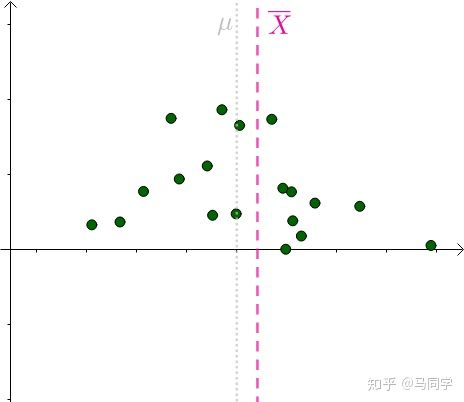
\includegraphics[width=15cm]{figure2.png}
\end{figure}
\begin{itemize}
    \item 第1层:软件系统。第一个层次就是整个系统,需要分解为子系统或包。
    \item 第2层:子系统或包。这一层的主要设计活动,就是确定如何把整个系统分为主要的子系统,并且定义
    清楚允许各子系统,如何使用其他子系统。这些子系统可能会很大,比如数据库、用户界面、业务规则、
    命令解释器、报表引擎等。在这一层的设计中,子系统之间的相互通信规则特别重要。如果所有的子系统
    都能和其他子系统通信,就完全失去了把它们分开所带来的好处。因此,应该通过限制子系统之间的
    通信,来让每个子系统更有存在的意义。
    \par
    例如,如下图所示,假设将系统分为6个子系统。在没有定义任何规则时,热力学第二定律就会发生作用,
    整个系统将会熵增。熵增的一种原因是,如果不对子系统间的通信加以任何限制,那么它们之间的通信就会
    肆意发生。
    \begin{figure}[ht]
        \centering
        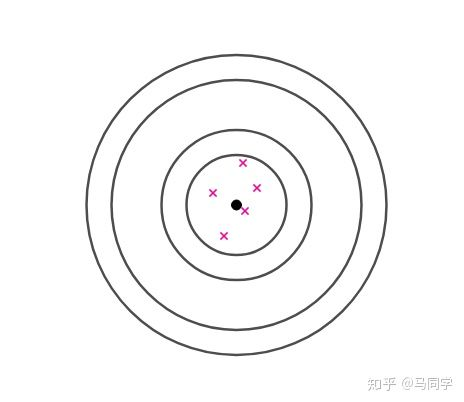
\includegraphics[width=10cm]{figure3.png}
    \end{figure}
    这里的每个子系统,最终都会直接与所有其他子系统进行通信,如果改动某一个子系统,则其他所有和其
    通信的子系统,都需要修改,这样是不合理的。因此需要限制子系统之间的通信,如下图所示,为施加了
    少量通信规则后的系统,
    \begin{figure}[ht]
        \centering
        
\includegraphics[width=10cm]{figure4.png}
    \end{figure}
    另外,为了让子系统之间的连接简单、易懂、且易于维护,就要尽量简化子系统之间的交互关系。最简单
    的交互关系,是让一个子系统,去调用另一个子系统中的子程序;稍微复杂一点的交互,是在一个子系统
    中,包含另一个子系统中的类;而最复杂的交互关系,是让一个子系统中的类,继承另一个子系统中的类。
    \par
    设计子系统,有一条很好的基本原则,即系统层设计图,应该是无环图;亦即程序中不应该有任何环形关系,
    比如说A类使用了B类、B类使用了C类、而C类又实用了A类这种情况。
    \par
    有些种类的子系统,会在不同的系统中反复出现,例如:
    \begin{itemize}
        \item 业务规则:指那些在计算机系统中,编入的法律、规则、政策以及过程;
        \item 用户界面:应创建一个子系统,把用户界面组件,同其他部分分隔开,以便用户界面的演化
        不会破坏程序的其余部分;在大多数情况下,用户界面子系统会使用多个附属的子系统或类,来处理
        用户界面、命令行接口、菜单操作、窗体管理、帮助系统等等;
        \item 数据库访问:可以将对数据库访问的实现细节隐藏起来,让程序的绝大部分,可以不必关心处理
        底层结构的繁琐细节,并能像在业务层次一样处理数据;
        \item 对系统的依赖性:把对操作系统的依赖因素,归到一个子系统里,就如同把对硬件的依赖因素,封装
        起来一样。例如,开发的程序不仅能在windows上运行,也应该可以方便地移植到linux或Mac OS上,
        且只需要修改接口子系统就可以了。
    \end{itemize}
    \item 第3层:分解为类。这一层的主要设计任务,是把所有的子系统,进行适当的分解,并确保分解出的
    细节都恰到好处,能够用单个的类实现。当定义子系统中的类时,也就同时定义了这些类与系统其余部分打交道
    的细节,尤其是要确定好类的接口。例如,数据库子系统可能会被进一步划分成数据库访问类、持久优化
    框架类、以及数据库元数据。
    \par
    类与对象的比较:面向对象设计的一个核心概念,就是对象(object)与类(class)的区分。对象是指运行
    期间,在程序中实际存在的具体实体,而类是指在程序源码中,存在的静态事物。对象是动态的,它拥有
    你在程序运行期间所能得到的具体的值和属性。例如,你可以定义一个名为Person的类,它具有姓名、
    年龄、性别等属性,在程序运行期间,你可以有nancy、hank、tony等对象,它们是类的具体实例。
    \item 第4层:分解成子程序。这一层的设计,包括把每个类细分为子程序(函数)。在第3层中,定义出
    类的接口,已经定义了其中一些子程序,而该层的设计,将细化出类的其他子程序。当你查看类里面
    子程序的细节时,就会发现很多子程序都很简单,但也有些子程序,是由更多层次的子程序所组成,这就
    需要更多的设计工作了。这一层次的分解和设计,通常是留给程序员个人来完成的。
    \item 第5层:子程序内部的设计。这里的设计工作,包括编写伪代码、选择算法、组织子程序内部的
    代码块,以及用何种编程语言编写代码。
\end{itemize}

\subsection{启发式设计方法}
由于软件设计是非确定性的,因此,灵活熟练地运用一组有效的启发式方法,便成了合理的软件设计核心工作。
\par
(1)找出现实世界中的对象:
\par
在确定设计方案时,首选且最流行的是面向对象的设计方法。此方法的要点是辨明现实世界中的对象,以及
人造的对象。使用对象设计的步骤:
\begin{itemize}
    \item 辨识对象及其属性:计算机程序通常都是基于现实世界的实体。例如,如下图所示,可以基于
    现实世界中的雇员(Employee)、顾客(Client)、工作时间记录(Timecard)、以及账单(Bill)等实体,
    来开发一套按时间计费的系统;
    \begin{figure}[ht]
        \centering
        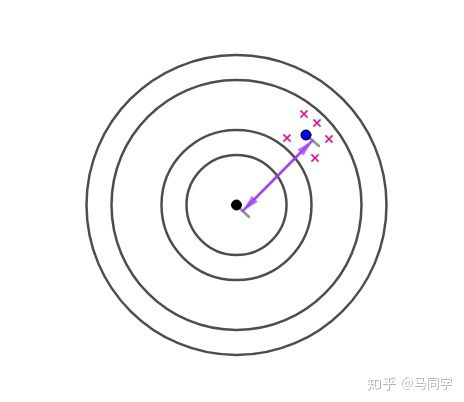
\includegraphics[width=10cm]{figure5.png}
    \end{figure}
    辨识对象的属性,并不比辨识对象本身更困难。每个对象都有一些与计算机程序相关的特征。例如,在这个
    收费系统里,每个雇员对象都具有名字(name)、职务(title)和费率(billingRate)等属性;而顾客对象
    则具有名字(name)、账单寄送地址(billingAddress)、以及账户余额(accountBalance)的属性;账单
    对象具有收费金额、顾客名字、支付日期(billDate)等等。
    \item 确定可以对各个对象进行的操作:在每个对象上,都可以执行多种操作;例如,雇员对象可能需要
    修改职务或者费率,顾客对象可能需要修改名字,或者账单寄送地址等等;
    \item 确定各个对象能对其他对象进行的操作:对象之间最常见的两种关系是包含和继承;一个Timecard
    对象可以包含一个Employee对象和一个Client对象,一个Bill对象可以包含一个或多个Timecard对象;
    另外,一份账单可以标示是否已经给某位顾客开过账单了,而顾客也可以签付一份账单;
    \item 确定对象的哪些部分,对其他对象可见:哪些部分是public的,哪些是private的;
    \item 定义每个对象的public接口:在编程语言的层次上,为每个对象定义具有正式语法的接口。对象对
    其他对象暴露的数据及方法,都被称为该对象的“public接口”,而对象通过继承关系,向其派生
    对象暴露的部分,则被称为“protected接口”。
\end{itemize}
经过上述这些步骤得到一个高层次的、面向对象的系统组织结构之后,你可以用这两种方法来迭代:在高层次的
系统组织结构上进行迭代,以便更好地组织类的结构;或者在每个已经定义好的类上进行迭代,把每个类的设计
详细化。

\par
(2)形成一致的抽象:
\par
抽象是一种能让你在专注某一概念的同时,可以放心地忽略其中一些细节的能力,
即在不同的层次处理不同的细节。任何时候,当你在对一个聚合物品操作时,就是在用抽象了。例如,当你
把一个东西称为“房子”,而不是由玻璃、木材和钉子构成的组合体时,就是在用抽像了。
\par
基类也是一种抽像,它使你能集中精力关注一组派生类所具有的共同特性,并在基类的层次上,忽略各个具体派生
类的细节;一个好的接口也是一种抽象,它能让你关注于接口本身,而不是类的内部工作方式。
\par
如下图所示,抽象是我们用来处理现实世界复杂度的一种重要手段;软件开发人员有时就是在木材纤维、
油漆分子,以及铁原子这一层来构建系统,因此就变得异常复杂,难以通过人的智力去管理;优秀的程序员
会在子程序接口的层次上、在类接口层次上,以及包接口的层次上进行抽象,这样才能更快、更稳妥地进行开发。
\begin{figure}[ht]
    \centering
    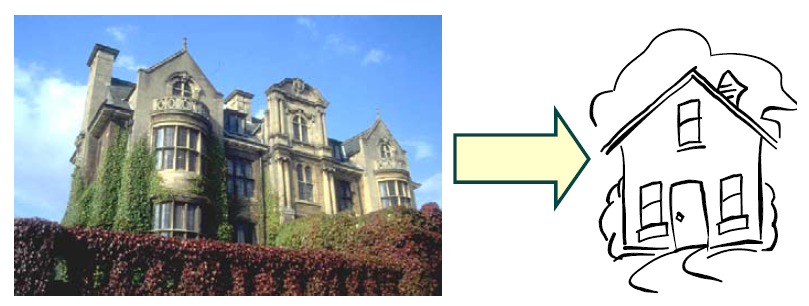
\includegraphics[width=15cm]{figure6.png}
\end{figure}

\par
(3)封装实现细节:
\par
封装填补了抽象留下的空白;抽象是指,可以让你从高层的细节,来看待一个对象;而封装则是指,除此
之外,你不能看到对象的任何其他细节层次。例如,如下图所示,封装是指,你可以从房屋的外面看,但
不能靠得太近,去将门的细节都看清楚;可以让你知道哪里有门,门是开还是关,但不能让你知道门是
木质的还是钢质的。
\begin{figure}[ht]
    \centering
    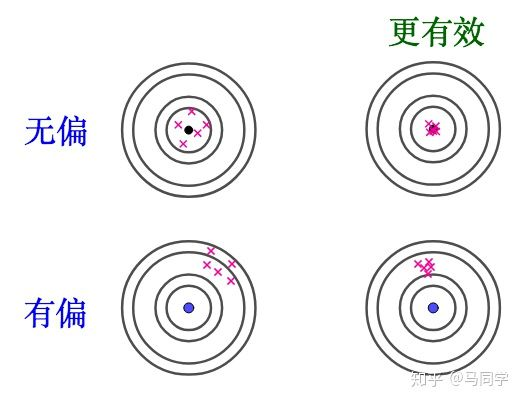
\includegraphics[width=15cm]{figure7.png}
\end{figure}

\par
(4)当继承能简化设计时就继承:
\par
在设计软件系统时,经常会发现一些大同小异的对象。例如,在一套账务系统中,包含全职员工和兼职员工,
两者的大多数数据是相同的,只是某些数据不同。在面向对象编程时,可以定义一个代表普通员工的通用类
型(general),然后把全职员工定义为普通员工,除了有一些不同之处;同样,把兼职员工也定义为普通员工,
除了一些不同之处;当一项针对员工的操作,与具体的员工类别无关时,这一操作就可以针对通用员工类型来
进行。当该操作需要区别全职员工和兼职员工时,就需要按照不同的方法来处理了。定义这种对象之间的相同点
和不同点,就叫“继承”,因为全职员工和兼职员工,都从基本员工类型继承了某些特征。
\par
继承的好处在于,它能很好地辅佐抽象的概念,并且能简化编程;因为你可以写一个基本的子程序,来处理
只依赖于门的基本属性的事项,另外写一些特定的子程序,来处理依赖特定种类门的特定操作。例如,
有些操作,如Open()或Close(),对于任何种类的门都能用,无论是防盗门还是玻璃门;编程语言如果能
支持像Open()或Close()这种,在运行期间才能确定所针对的对象的实际类型的操作,这种能力叫做
“多态”。

\par
(5)信息隐藏:
\par
信息隐藏是降低软件复杂度的一种格外重要的启发式方法,因为它强调的就是隐藏复杂度。
\begin{itemize}
    \item 隐私权:当信息被隐藏后,每个类或子程序都代表了,某种对其他类保密的设计或构建决策。
    隐藏起来的秘密,可能是某个易变的区域,或者某种文件格式,或某种数据类型的实现方式,或某个
    需要隔离的区域,在这个区域中发生的错误,不会给程序其余部分带来太大损失。在这里,类的职责
    就是把部分信息隐藏起来,并保护自己的隐私权。对系统的非重大改动,可能会影响到某个类中的
    几个子程序,但它们不应该波及到类接口的外面。
    \par
    在设计类的时候,一项关键的决策,就是确定类的哪些信息应该对外可见,而哪些信息应该隐藏起来。
    如下图所示,类的接口应该尽可能少地暴露其内部工作机制。设计类的接口与设计其他环节一样,都是
    一个迭代的过程;如果你第一次没有得到合适的接口,那么就多试几次,知道设计稳定下来;如果设计仍不
    稳定,那就需要换种方法再尝试。
    \begin{figure}[ht]
        \centering
        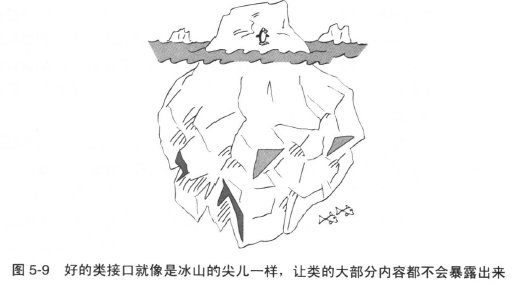
\includegraphics[width=10cm]{figure8.png}
    \end{figure}
    \item 信息隐藏的一个例子:假设你有一个程序,其中的每个对象,都是通过一个名为id的成员变量
    来保存一种唯一的ID。一种设计方法,是用一个整数来表示ID,同时用一个名为g\_maxId的全局变量,来保存
    目前已分配的ID的最大值。每当创建新的对象时,你只要在该对象的构造函数里,简单地使用
    id=++g\_maxId这条语句,就可以获得一个唯一的ID值,这种做法会让对象在创建时,执行的代码量
    最少。可这样设计可能会出错:如果你像把某些范围的ID留作它用该怎么办?如果想用非连续ID来
    提高安全性又该怎么办?如果你想重新使用已销毁对象的ID呢?如果你想增加一个断言,来确保所分配
    的ID不会超过预期的最大范围呢?如果程序中到处都是id=++g\_maxId这种语句,一旦上面说的任何
    一种情况出现,就需要修改所有这些语句。另外如果程序是多线程的,这种方法也不是线程安全的。
    \par
    创建新ID的方法就是一种你应该隐藏信息的设计决策。如果你在程序中到处使用++g\_maxId的话,就暴露
    了创建新ID的方法,即通过简单递增的方式;想法,如果你在程序中,使用语句id=NewId(),那就把创建
    新ID的方法隐藏起来了。你可以在NewId()子程序中仍然只用一行代码,return (++g\_maxId),或者
    其他与之等价的方法。如果想修改,只需修改NewId()即可。
    \par
    现假设需要把ID的类型由int改为字符串,如果在程序中大量使用了针对int的操作,例如>、<、=等等,
    这些操作并不适用字符串,那么即使改用NewId()子程序,也无济于事。因此,另一个需要隐藏的信息,就是
    ID的类型。在C++里,可以简单地使用typedef来把ID定义为IdType,也可以创建一个简单的IdType类。
    \par
    隐藏设计决策,对于减少“改动所影响的代码量”,是至关重要的。信息隐藏在设计的所有层次上,都有很大作用,
    从使用具名常量替代字面量,到创建数据类型,再到类的设计、子程序的设计以及子系统的设计等等。
    \item 两种信息:信息隐藏中所说的信息主要分为两大类,复杂度和变化源;
    \item 信息隐藏的障碍:
    \begin{itemize}
        \item 信息过度分散。例如,将100这个数字直接写到程序各个地方,会导致对它的引用过度分散;
        最好将它写入MAX\_EMPLOYEES的常量中,如果需要改动,只需要改动一处即可;
        \item 循环依赖。例如,A类中的子程序,调用了B类的中的子程序;然后B类中的子程序,又调用
        A类中的子程序;
        \item 将类内数据误认为全局数据。为了避免全局数据可能带来的问题,将类内数据误认为全局数据,
        并避免使用它。全局数据通常会受困于两类问题:一种是子程序在全局数据上执行操作,却不知道
        还有其他子程序也在用这些全局数据进行操作;另一种是子程序知道其他子程序也在用全局数据进行
        操作,但却无法明确地知道都进行了哪些操作。而类内数据就不会有这种问题,因为只有类内部的
        少数子程序才能直接访问这些数据。这些子程序不但知道有其他子程序在操纵这些数据,而且也明确
        知道具体是哪些子程序在执行这些操作。但如果设计的类包含很多体积庞大的众多子程序,那么类
        数据和全局数据之间的区别就变得模糊起来,类内数据也将开始受困于全局数据所面临的那些问题了。
        \item 可以察觉的性能损耗。如果在架构层按照信息隐藏的目标去设计系统,并不会与按照性能目标
        去设计想冲突,因此在系统架构层和编码层均避免性能上的损耗。
    \end{itemize}
    \item 信息隐藏的价值:运用了信息隐藏技术的大型项目,与没有应用这一技术的项目,修改起来大约
    容易4倍;而且信息隐藏还是结构化程序设计和面向对象设计的根基之一。
\end{itemize}

\par
(6)找出容易改变的区域:
\par
程序设计面临的最重要挑战之一,就是适应变化。需要将不稳定的区域隔离出来,从而把变化所带来的影响,
限制在一个子程序、类或包的内部。可采取的应对各种变动的措施:
\begin{itemize}
    \item 找出看起来容易变化的项目。如下是一些容易发生变化的地方:
    \begin{itemize}
        \item 业务规则:业务规则很容易成为软件频繁变化的根源。国会改变了税率结构,保险公司改变
        了它的税率表等等;如果你遵循信息隐藏的原则,那么基于这些业务规则的逻辑,就不应该遍布于整个
        程序,而是仅仅隐藏在系统的某个角落,知道需要对它进行改动,才会把它拎出来;
        \item 对硬件的依赖:与屏幕、键盘、鼠标设施以及通信设计等之间的接口,都是硬件依赖的例子。请把
        对硬件的依赖,隔离在它们自身的子系统或类中。这种隔离非常有利于把你的程序移植到新的硬件环境下。另外,
        当你为可能变化的硬件开发程序时,这样做也会有很大帮助。你可以写软件来模拟与特定硬件的交互,
        在硬件尚不稳定,或者不可用的时候,让硬件接口子系统使用该模拟器,当硬件可用的时候,把硬件接口
        子系统与模拟器切断,最终连接到真正的硬件设备上;
        \item 输入和输出:在做比纯硬件接口层稍高一些层面上的设计时,输入输出也是一个容易变化的区域。
        如果你的程序创建了自己的数据文件,那么该文件格式就可能会随软件开发的不断深化而变化。用户层
        的输入和输出格式也会变化:输出页面上字段位置、数量和排列顺序等都可能会变。因此,检查所有
        的外部接口,看看有哪些可能的变化,通常是个不错的主意;
        \item 非标准的语言特性:大多数编程语言的实现中,都包含了一些便利的、非标准的扩展。这些扩展
        可能在其他的环境中不可用;因此需要将这样的扩展单独隐藏在某个类里,以便当你转移到新的环境后,
        可以用自己写的代码区取代。与此类似,如果你使用了并非所有环境中都可用的函数库,请把这些子程序
        库隐藏在一个接口的后面,为新环境做好准备;
        \item 困难的设计区域和构建区域:将困难的设计区域和构建区域隐藏起来,也是很好的想法,因为
        这些代码可能因为设计得很差,而需要重新做;
        \item 状态变量:状态变量用于表示程序的状态,与大多数其他的数据相比,这种东西更容易改变;
        在一个典型的应用场景里,你可能一开始用布尔变量,来定义出错状态,然后又发现用具有ErrorType\_None、
        ErrorType \_Warning和ErrorType\_Fatal等值的枚举类型,来表示该状态更好。
        可以在使用状态变量时,增加至少两层的灵活性和可读性:
        \begin{itemize}
            \item 不要使用布尔变量作为状态变量,而是用枚举类型;
            \item 使用访问器子程序检查状态变量,而不是直接检测;
        \end{itemize}
        \item 隐藏数据量:例如用具名常量MAX\_EMPLOYEES来隐藏100这样的数字。
    \end{itemize}
    \item 把容易变化的项目分离出来。将容易变化的组件,单独划分成类,或者和其他容易同时发生变化的
    组件,分到同一个类中。
    \item 把容易变化的项目隔离开来。设计类之间的接口,使其对潜在的变化不敏感。
\end{itemize}
找出容易发生变化区域的一个好办法:首先找出程序中可能对用户有用的最小子集。这一子集构成了系统的
核心,不容易发生变化。接下来,用微小的步伐扩充这个系统。这里的增量可以非常微小,小到看似微不足道。
当你考虑功能上的改变时,同时也要考虑质的变化:比如让程序变成线程安全,使程序能够本地化等。这些潜在
的改进区域,就构成了系统中的潜在变化。请依照信息隐藏的原则,来设计这些区域。通过首先定义清楚核心,
你可以认清哪些组件属于附加功能,这是就可以把它们提取出来,并把它们的可能改进隐藏起来。

\par
(7)保持松散耦合:
\par
耦合度表示类与类之间,或子程序与子程序之间的关系紧密程度。耦合度设计的目标,是创建出小的、直接的、
清晰的类或子程序,使它们与其他类或子程序之间,关系尽可能地灵活,这就被称作“松散耦合”。模块之间
良好的耦合关系,需要松散到恰好能使一个模块,能够很容易地被其他模块使用,确保模块之间的连接关系
尽可能的简单。尽量使创建的模块,不依赖或很少依赖其他模块。例如sin()这样的子程序是松耦合的,因为它
需要知道的东西,也就是一个传入的、代表角度的数值。而像InitVars(var1,...,varN)这样的子程序,则耦合
得过于紧密,因为在调用端,必须传入各个参数,调用它的模块实际上知道在InitVars()内部会做些什么。
如果两个类都依赖于同一个全局变量的使用,那么它们之间的耦合关系就更紧密了。
\begin{itemize}
    \item 耦合标准:下面是一些在衡量模块之间耦合度使,可采用的标准
    \begin{itemize}
        \item 规模。指模块之间的连接数。只有1个参数的子程序,相比有6个参数
        的子程序,耦合度更高;
        \item 可见性。指两个模块之间,连接的显著程度。在程序开发过程中,需要把模块之间的连接关系,
        变得广为人知而获取信任。通过参数表传递数据,则是一种明显连接,值得提倡;而通过修改全局数据,
        进而使另一个模块能使用该数据,则是一种不好的设计;
        \item 灵活性。指模块之间的连接,是否容易改动。一个模块越容易被其他模块调用,那么它们之间
        的耦合关系,就会越松散,并且更易于维护。因此,在创建系统架构时,应按照“尽可能缩减相互连接”的
        准则,来分解程序。
    \end{itemize}
    \item 耦合种类:几种常见的几种耦合,
    \begin{itemize}
        \item 简单数据类型的参数耦合。当两个模块之间,通过参数来传递数据,并且所有的数据都是简单
        数据类型时,这两个模块之间的耦合关系,就是简单数据参数耦合的。这种耦合关系是正常且可以接受的。
        \item 简单对象耦合。如果一个模块实例化一个对象,那么它们之间的耦合关系,就是简单对象耦合的。
        这种耦合关系也很不错。
        \item 对象参数耦合。如果Object1要求Object2传给它一个Object3,那么这两个模块就是对象参数耦合的。
        与Object1仅要求Object2传递给他简单数据类型相比,这种耦合关系要更紧密些,因为它要求Object2
        了解Object3。
        \item 语义上的耦合。最难缠的耦合关系是这样发生的:一个模块不仅使用了另一个模块的语法元素,
        而且还使用了有关那个模块内部工作细节的语义知识。例如Module1向Module2传递了一个控制标志,
        用它告诉Module2该做什么,这种方法要求Module1对Module2的内部工作细节有所了解,也就是说需要
        了解Module2对控制标志的使用。语义上的耦合是非常危险的,因为更改被调用模块中的代码,可能会
        破坏调用它的模块,破坏的方式是编译器完全无法检查的。类似这样的代码崩溃时,其方式是非常微妙的,
        看起来与被使用的模块中的代码更改毫无关系,因此会使得调试工作变得无比困难。
    \end{itemize}
\end{itemize}
\par
松散耦合的关键之处在于,一个有效的模块提供了一层附加的抽象:一旦你写好了它,就可以想当然地去用它。
这样就降低了整体系统的复杂度,使得你可以在同一时间,只关注一件事。如果对一个模块的使用,要求你
同时关注好几件事:其内部工作的细节、对全局数据的修改、不确定的功能点等;那么就失去了抽象的能力,
模块所具有的管理复杂度的能力也就削弱或完全丧失了。

\par
(8)查阅常用的设计模式:
\par
设计模式精炼了众多现成的解决方案,可以解决很多软件开发中,最常见的问题。有些软件问题要求
全新的解决方案,但是大多数问题都和过去遇到的问题类似,因此可以使用类似的解决方案或者模式加以解决。
下表为常见的设计模式:
\begin{figure}[ht]
    \centering
    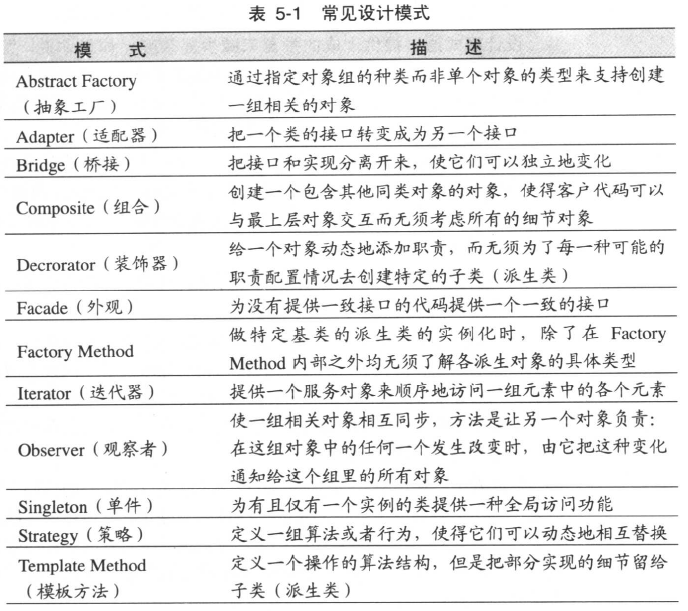
\includegraphics[width=10cm]{figure9.png}
\end{figure}
\par
与完全定制的设计方案相比,设计模式提供了下列好处:
\begin{itemize}
    \item 设计模式通过提供现成的抽象,来减少复杂度;
    \item 设计模式通过把常见解决方案的细节,通过制度化来减少出错;
    \item 设计模式通过提供多种设计方案,带来启发性的价值;
    \item 设计模式通过把设计对话,提升到一个更高的层次上,来简化交流。
\end{itemize}
\par
应用设计模式的一个潜在陷阱,是强迫让代码适用于某个模式。有时候,对代码进行一些微小的更改,
以便符合某个广为人知的模式,会使这段代码更容易理解。但是,如果一段代码做出巨大改动,迫使它
去符合某个标准设计模式,有时反而会把问题复杂化。

\par
(9)使用启发式方式的原则:
\par
最有效的原则之一,就是不要卡在单一的方法上。如果用UML画设计图不可行,那么就直接用英语写;
写段简短的测试程序;尝试一种截然不同的方法;用铅笔画出轮廓和草图来指导思维等等。
\par
你无须马上解决整个设计难题。一旦被卡住了,那么请记住回过头来时,有一处地方需要做决策,但眼下
你还没有足够的信息来解决这个问题。如果你尝试了一些设计方案,但没有很好的解决问题的时候,更自然
的方式,是让那些问题留在未解决的状态,等拥有更多信息后,在去做。

\subsection{设计实践}
在设计过程中,可以采用如下一些工作步骤,以便获得良好的设计结果:
\par
(1)迭代
\par
设计是一个迭代的过程。当在备选的方案之中,循环并尝试一些不同的做法时,将会同时从高层和低层的不同
视角,去审视问题。从高层视角从得到的大范围图景,有助于你把相关的低层细节纳入考虑;从低层视角中
获得的细节,也会为你的高层决策奠定基础。这种高低层面之间的互动,被认为是一种良性的原动力,它
所创建的结构,要远远稳定于单纯自上而下,或自下而上创建的结构。

\par
(2)分而治之
\par
没有人的头脑能装下一个复杂程序的全部细节,对设计同样适用。将程序分解为不同的关注区域,然后
分别处理每一个区域;如果在某个区域里碰上了死胡同,那么就迭代。

\par
(3)自上而下和自下而上
\begin{itemize}
    \item 自上而下的设计:是指从某个很高的抽象层次开始,定义出基类或其他不那么特殊的设计元素;在开发
    这一设计的过程中,逐渐增加细节的层次,找出派生类、合作类,以及其他更细节的设计元素。
    这种设计方式可以看作是一层层分解的过程,在分解过程的不同阶段,需要选择用什么方法,去分解
    子系统,给出继承关系树,形成对象的组合。持续分解,直到在下一层,直接编码比分解更容易。
    \item 自下而上的设计:是指设计始于细节,向一般性延伸;这种设计通常是从寻找具体对象开始,最后从细节之中生成
    对象以及基类。需要考虑的一些步骤:
    \begin{itemize}
        \item 对系统需要做的事项,有哪些已知条件;
        \item 找出具体的对象和职责;
        \item 找出通用的对象,把它们按照适当方式组织起来:子系统、包、对象组合,或者继承;看哪种方式合适;
        \item 在更上一层继续设计,或者回到最上层,尝试向下设计
    \end{itemize}
    \item 两者并不矛盾:两种策略最关键的区别在于,自上而下是一种分解策略;而自下而上是一种合成策略;
    前者从一般性的问题出发,把该问题分解成可控的部分;后者从可控的部分出发,去构造一个通用的方法。
\end{itemize}

\par
(4)建立试验性原型
\par
有些时候,除非能很好的了解实现细节,否则很难判断一种设计方法是否凑效。例如,在知道它能满足性能要求
之前,很难判断某种数据库的组织结构是否适用。此时,建立试验性原型,便能低成本解决这些问题:写出用于
回答特定设计问题的、量少且能够随时扔掉的代码。但是使用试验原型,存在以下一些风险:
\begin{itemize}
    \item 开发人员没有遵循“用最少代码回答提问”的原则。例如,设计问题是“我们选的的数据库框架,
    能否支撑所需的交易量?”,你不需要为了这一问题,而编写任何产品代码,也不需要去了解数据库的详情;
    只需要了解能估计出问题范围的最少信息:有多少张表、表中有多少条记录等等,接下来就可以用Table1、
    Table2、Column1、Column2等名字,写出最简单的原型代码,往表里随意填入些数据,然后做你所
    需要的性能测试;
    \item 设计的问题不够特殊。例如,设计问题“这样的数据库框架,能否工作?”,并没有为建立原型提供多少
    指引;而像“这个数据库框架能不能在X、Y和Z的前提下,支持每秒1000次交易?”这样的问题,则能
    为建立原型,提供更坚实的基础;
    \item 开发人员不把原型代码当作可抛弃的代码。如果开发人员相信某段代码,将被用在最终产品里,
    那么他根本不可能写出最少数量的代码来。避免产生这一问题的一种做法,是用与产品代码不同的技术,
    来开发原型。例如用Python来为C++设计做原型。
\end{itemize}


\par
(5)合作设计
\par
无论组织形式的正式与否,在设计过程中,三个臭皮匠顶得上一个诸葛亮,合作可以以任意方式展开。例如,
随便走到一名同事办公桌前,向他征求一些想法;结对编程等等。


\par
(6)做多少设计才足够
\par
对于实施正式编码前的设计工作量和设计文档的正规程度,很难有个确定的定论,下表可以做个参考,
\begin{figure}[ht]
    \centering
    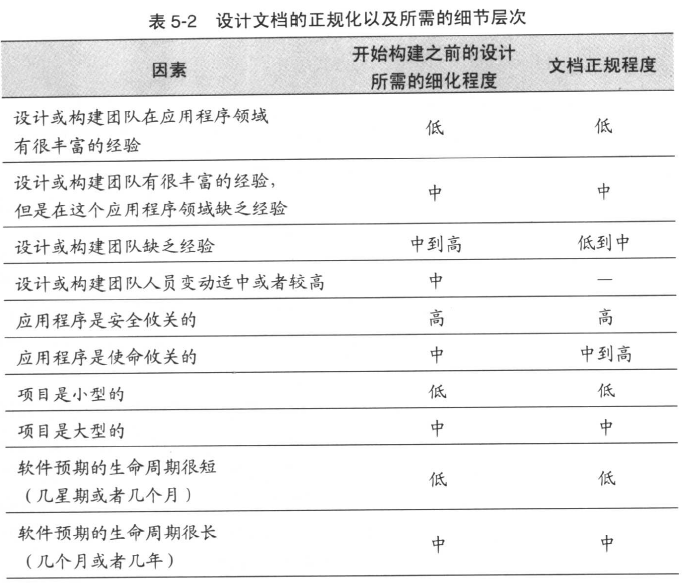
\includegraphics[width=10cm]{figure10.png}
\end{figure}
\par
如果在编码前,还没法判断是否应该做更多深入设计,那么宁愿去做更详细的设计。最大的设计失误,来自于
误认为自己已经做得很充分,可事后却发现还是做得不够。另一方面,也不要太过于专注,对设计进行文档化,
而导致失败;程序化的活动,容易把非程序化的活动驱逐出去,过早地去润色设计方案,就是所描述的例子。

\par
(7)记录设计成果
\par
传统的记录设计成果的方式,是把它写成正式的设计文档;然而,你还可以用很多种方法来记录设计成果,
这些方法对于那些小型的、非正式项目,或者只需要轻量级地记录设计成果的项目,效果是很不错的:
\begin{itemize}
    \item 把设计文档插入到代码里:在代码注释中写明关键的设计决策,通常放在文件或类的开始位置;
    \item 用Wiki来记录设计讨论和决策;
    \item 写总结邮件;
    \item 使用数码相机;
    \item 保留设计挂图;
    \item 使用CRC卡片(类、职责、合作者);
    \item 在适当的细节层,创建UML图。
\end{itemize}


\section{可以工作的类}
类是由一组数据和子程序构成的集合,这些数据和子程序共同拥有一组内聚的、明确定义的职责。类也可以
只是由一组子程序构成的集合,这些子程序提供一组内聚的服务,哪怕其中未涉及共用的数据。成为高效
程序员的一个关键,在于当你开发程序任一部分的代码时,都能安全地忽视程序中尽可能多的其余部分。
而类就是实现这一目标的首要工具。

\subsection{类的基础:抽象数据类型}
抽象数据类型(ADT,abstract data type)是指一些数据,以及对这些数据所进行的操作的集合。这些操作,
既是像程序的其余部分描述了这些数据是怎么样的,也允许程序的其余部分改变这些数据。一个ADT可能是一个图形
窗体,以及所有能影响该窗体的操作;也可以是一个文件,以及对这个文件进行的操作等等。
\par
(1)一个ADT例子:
\par
假如你正在写一个程序,控制文本的字体,它能用不用的字型、字号等;如果用一个ADT,就能在相关数据上,
捆绑一组操作字体的子程序;相关的数据包括字体名称、字号和文字属性等。这些子程序和数据集合,就是
一个ADT。
\par
如果不使用ADT,就只能用一种拼凑的方法来操纵字体了。例如,如果要将字体大小改为12磅(point),
即高度为16像素(pixel),那么就需要这样的代码:
\par
currentFont.sizeOnPixels = PointsToPixels(12)
\par
\noindent 但不能同时使用currentFont.sizeInPixels和currentFont.sizeInPoints;因为如果你同时使用
这两项数据成员,currentFont就无从判断到底该用哪个。而且,如果你在程序很多地方都需要修改字体
大小,那么这类语句就会散步在整个程序中。如果需要把字体设为粗体,或许需要写成这样:
\par
currentFont.attribute = CurrentFont.attribute or 0x02 或
\par
currentFont.bold = True
\par
\noindent 这些做法都存在一个限制,即要求调用方代码,直接控制数据成员,这无疑限制了currentFont的使用。

\par
(2)使用ADT的好处
\par
\begin{itemize}
    \item 可以隐藏实现细节:把信息隐藏起来,能保护程序的其余部分不受影响。
    \item 改动不会影响到整个程序:如果数据类型改变,只需在一处修改而不会影响到整个程序。
    \item 让接口能提供更多信息:把所有相似的操作,都集中到一个ADT中,就可以基于磅数或像素
    来定义整个接口,或者把二者明确区分开,从而有助于避免混淆。
    \item 更容易提高性能:如果想提高操作字体时的性能,就可以重新编写出一些更好的子程序,
    而不用来回修改整个程序。
    \item 让程序的正确性更显而易见:验证像currentFont.attribute = CurrentFont.attribute or 0x02
    的语句是否正确,是很枯燥的,可以替换成像currentFont.SetBoldOn()这样的语句,验证它
    是否正确就更容易一些。
    \item 程序更具自我说明性:可以改进currentFont.attribute = CurrentFont.attribute or 0x02
    这样的语句:将0x02换成BOLD,但无论怎么杨修,其可读性都不如currentFont.SetBoldOn()
    这条语句。
    \item 无须在程序内到处传递数据:在上面的例子中,必须直接修改currentFont的值,或把它传给
    每一个要操作字体的子程序;如果使用了ADT,就不用再在程序里到处传递currentFont了。
    \item 可以像在现实世界中那样操作实体,而不用在底层实现上操作它:可以定义一些针对字体
    的操作,这样程序的绝大部分,就能完全以“真实世界中的字体”这个概念来操作,而不再用数组访问、结构体
    定义、True与False等这些底层的实现概念了。
\end{itemize}
为了定义一个ADT,只需要定义一些用来控制字体的子程序,例如:
\par
currentFont.SetSizeInPoints(sizeInPoints)
\par
currentFont.SetSizeInPixels(sizeInPixels)
\par
currentFont.SetBoldOn()
\par
currentFont.SetBoldOff()

\par
(3)使用ADT的一些建议:
\par
\begin{itemize}
    \item 把常见的底层数据类型构建为ADT,并使用这些ADT,而不再使用底层数据类型:堆栈、列表、
    队列,以及几乎所有常见的底层数据类型,都可以用ADT表示;如果堆栈代表的是一组员工,就该把它
    看作是一些员工,而不是堆栈;如果列表代表一个出场演员名单,就该把它看作是出场演员名单,而不是列表等等。
    \item 把像文件这样的常用对象当成ADT。
    \item 简单的事物也可当作ADT:例如,一盏灯只有开和关两种操作,也可以放到ADT里,这样可以
    提高代码的自我说明能力,并减少需要到处传递的数据。
    \item 不要让ADT依赖于存储介质:假设有一张保险费率表,它太大了,因此只能保存在磁盘上;
    你可能编写出rateFile.Read()这样的访问器子程序,然而当你把它当作一个“文件”时,就已经暴露
    了过多的数据信息,一旦对程序进行修改,把这张表存到内存中,而不是磁盘上,把它当作文件的
    那些代码将不正确,而且产生误导并使人迷惑。因此,请尽量让类和访问器子程序的名字,与存储数据的方式
    无关,并只提及抽象数据类型本身,例如rateTable.Read()或更简单rates.Read()。
\end{itemize}

\subsection{良好的类接口}
创建高质量的类,第一步,可能也是最重要的一步,就是创建好的接口。这也包括了创建一个可以通过接口来
展现的合理抽象,并确保细节仍被隐藏在抽象背后。
\par
(1)好的抽象:
\par
抽象是一种以简化的形式,来看待复杂操作的能力。类的接口为隐藏在其后的具体实现,提供了一种抽象。
类的接口应能提供一组明显相关的子程序。
\par
假设有一个实现雇员(Employee)这一实体的类,其中可能包含雇员的姓名、地址、电话号码等数据,以及一些用
来初始化并使用雇员的服务子程序,例如:
\begin{lstlisting}
    C++示例:展现良好抽象的类接口
    class Employee {
    public:
        // public constructors and destructors
        Employee();
        Employee(
            FullName name,
            String address,
            String workPhone,
            String homePhone,
            TaxId taxIdNumber,
            JobClassification jobClass
        );
        virtual ~Employee();
        // public routines
        FullName GetName() const;
        String GetAddress() const;
        String GetWorkPhone() const;
        String GetHomePhone() const;
        TaxId GetTaxIdNumber() const;
        JobClassification GetJobClassification() const;
        ...
    private:
        ...
    };
\end{lstlisting}
在类的内部,还可能会有支持这些服务的其他子程序和数据,但类的使用者,并不需要了解它们;类接口的
抽象能力非常有价值,因为接口中的每个子程序,都在朝这个一致的目标而工作。
\par
一个没有经过良好抽象的类,可能会包含有大量混杂的函数,例如
\begin{lstlisting}
    C++示例:展现不良抽象的类接口
    class Program {
    public:
        ...
        //public routines
        void InitializeCommandStack();
        void PushCommand( Command command );
        Command PopCommand();
        void ShutdownCommandStack();
        void InitializeReportFormatting();
        void FormatReport( Report report );
        void PrintReport( Report report );
        void InitializaeGlobalData();
        void ShutdownGlobalData();
        ...
    private:
        ...
    };
\end{lstlisting}
其中有很多子程序,有用来操作命令栈的,有用来格式化报表的,有用来打印报表的,还有用来初始化全局数据的。
在命令栈、报表和全局数据之间,很难看出什么联系。类的接口不能展现出一种一致的抽象,因此它的
内聚性就很弱;应该把这些子程序,重新组织到几个职能更专一的类里去,在这些类的接口中,提供更好的
抽象。
\par
如果这些子程序是一个叫做Program类的一部分,那么可以这样来修改它,以提供一种一致的抽象:
\begin{lstlisting}
    C++示例:能更好展现抽象的类接口
    class Program{
    public:
        ...
        // public routines
        void InitializeUserInterface();
        void ShutdownUserInterface();
        void InitializeReports();
        void ShubtdownReports();
        ...
    private:
        ...
    };
\end{lstlisting}
在清理这一接口时,将原有的一些子程序,转移到其他更适合的类里面,而把另一些转为InitializeUserInterface()
和其他子程序中使用的私有子程序。
\par
这种对类的抽象进行评估的方法,是基于类所具有的public子程序所构成的集合,即类的接口。即使类的
整体表现出一种良好的抽象,类内部的子程序也未必都能表现出良好的抽象,也同样要把它们设计得可以表现出
很好的抽象。
\par
一些创建类的抽象接口的指导建议:
\begin{itemize}
    \item 类的接口应该展现一致的抽象层次:在设计类的时候,有一种很好的方法,就是把类看作一种
    用来实现ADT的机制;每一个类应该实现一个ADT,并且仅实现这一个ADT。如果你返现某个类实现了不止
    一个ADT,或者你不能确定究竟它实现了何种ADT,你就应该把这个类,重新组织为一个或多个定义
    更加明确的ADT。
    \begin{lstlisting}
        C++示例:混合了不同层次抽象的类接口
        class EmployeeCensus: public ListContainer {
        public:
            ...
            // public routines
            void AddEmployee( Employee employee );
            void RemoveEmployee( Employee employee );

            Employee NextItemInList();
            Employee FirstItem();
            Employee LastItem();
            ...
        private:
            ...
        };
    \end{lstlisting}
    这个类展现了两个ADT:Employee和ListContainer。出现这种混合的抽象,通常是源于程序员使用容器类
    或其他类库来实现内部逻辑,但却没有把“使用类库”这一事实隐藏起来。下面是隐藏了实现细节的类接口:
    \begin{lstlisting}
        class EmployeeCensus {
        public:
            ...
            // public routines
            void AddEmployee( Employee employee );
            void RemoveEmployee( Employee employee );
            Employee NextEmployee();
            Employee FirstEmployee();
            Employee LastEmployee();
            ...
        private:
            ListContainer m_EmployeeList;
            ...
        };
    \end{lstlisting}
    \item 一定要理解类所实现的抽线是什么:一些类非常像,必须非常仔细地理解类的接口,应该捕捉的
    抽象到底是哪一个。当你不得不在两个相似的抽象之间做出选择时,请确保你的选择是正确的。
    \item 提供成对的服务:大多数操作都有和其相应的、相等的以及相反的操作。如果有一个操作用来把
    灯打开,那很有可能也需要另一个操作,来把灯关闭。在设计类的时候,需要检查每一个public子程序,
    决定是否需要另一个与其互补的操作。不要盲目地创建相反操作,但你一定要考虑,看看是否需要它。
    \item 把不相关的信息转移到其他类中:有时你会发现,某个类中,一般子程序使用着该类的一半数据,
    而另一半子程序则使用另一半数据。这时你其实已经把两个类混在一起使用了,这就需要把它们拆开。
    \item 尽可能让接口可编程,而不是表达语义:每个接口都由一个可编程的部分和一个语义部分组成。
    可编程的部分,由接口中的数据类型和其他属性构成,编译器在检查编译错误时,能强制性地要求它们。
    而语义部分则由“本接口将会被怎样使用”的假定组成,而这些是无法通过编译器来强制实施的。例如,
    语义接口中包含的考虑“RoutineA必须在RoutineB之前被调用”。语义接口应通过注释说明,但要尽可能
    让接口不依赖于这些说明。一个接口中任何无法通过编译器强制实施的部分,就是一个可能被误用的
    部分。要想办法把语义接口的元素,转换为编程接口的元素,比如用断言或其他的技术。
    \item 谨防在修改时破坏接口的抽象:在对类进行修改和扩展的过程中,常常会发现额外所需的一些功能;
    这些功能并不十分适应于原有的类接口,可看上去却很难用另一种方法实现。例如,上面的Employee类
    演变成了下面这个样子:
    \begin{lstlisting}
        C++语言示例:在维护时被破坏的类接口
        class Employee {
        public:
            ...
            // public routines
            FullName GetName() const;
            Address GetAddress() const;
            PhoneNumber GetWorkPhone() const;
            ...
            bool IsJobClassificationValid( JobClassification jobClass );
            bool IsZipCodeValid( Address address );
            bool IsPhoneNumberValid( PhoneNumber phoneNumber );
            SqlQuery GetQueryToCreatNewEmployee() const;
            SqlQuery GetQueryToModifyEmployee() const;
            SqlQuery GetQUeryToRetrieveEmployee() const;
            ... 
        private:
            ...
        };
    \end{lstlisting}
    前面代码示例中的清晰抽线,现在已经变成了,由一些零散功能组成的大杂烩。在雇员和检查邮政
    编码、电话号码或职位的子程序之间,并不存在什么逻辑上的关联,那些暴露SQL语句查询细节的子程序,
    所处的抽象层次比Employee类也要低得多,它们都破坏了Employee类的抽象。
    \item 不要添加与接口抽象不一致的公用成员:每次你向类的接口中,添加子程序时,问问“这个子程序
    与现有接口所提供的抽象一致吗”,如果发现不一致,就要换另一种方法来进行修改,以便能保持抽象的
    完整性。
    \item 同时考虑抽象性和内聚性:抽象性和内聚性这两个概念之间的关系,非常紧密:一个呈现出很好
    的抽象的类接口,通常也有很高的内聚性。而具有很强内聚性的类,往往也会呈现为很好的抽象。关注类的
    接口所表现出来的抽象,比关注类的内聚性更有助于深入地理解类的设计。如果你发现某个类的内聚性很弱,
    也不知道该怎么改,那就换一种方法,问问你自己这个类是否表现为一致的抽象。
\end{itemize}

\par
(2)良好的封装
\par
封装是一个比抽象更强的概念。抽象通过提供一个,可以让你忽略实现细节的模型,来管理复杂度;而封装则
强制阻止你看到细节,即便你想这么做。这两个概念之所以相关,是因为没有封装时,抽象往往很容易被打破。
依据经验,要么就是封装与抽象两者皆有,要么就是两者皆失。除此之外,没有其他可能。
\begin{itemize}
    \item 尽可能地限制类和成员的可访问性:让可访问性尽可能低,是促成封装的原则之一。当你在犹豫
    某个子程序的可访问性,应该设为public、private还是protected时,经验之举应该采用最严格且可行的
    访问级别。这是一个很好的指导建议,但还有更重要的建议,即考虑“采用哪种方式,最好地保护接口抽象
    的完整性?”,如果暴露一个子程序不会让抽象变得不一致的话,这么做就很可能是可行的。如果不
    确定,那么多隐藏,通常比少隐藏要好。
    \item 不要公开暴露成员数据:暴露成员数据会破坏封装性,从而限制你对这个抽象的控制能力。例如,一个Point
    类如果暴露了下面这些成员的话:
    \begin{lstlisting}
        float x;
        float y;
        float z;
    \end{lstlisting}
    它就破坏了封装性,因为调用该类可以自由地使用Point类里面的数据,而Point类却连这些数据什么
    时候被改动过都不知道。然而,如果Point类暴露的是这些方法的话:
    \begin{lstlisting}
        float GetX();
        float GetY();
        float GetZ();
        void SetX(float x);
        void SetY(float y);
        void SetZ(float z);
    \end{lstlisting}
    那它还是封装完好的。你无法得知底层实现用的是不是float x、y、z,也不会知道Point是不是把这些
    数据保存为double然后再转换成float,也不可能知道Point是不是把它们保存在月亮上,然后再从
    外层空间中的卫星上把它们找回来。
    \item 避免把私有的实现细节放入到类的接口中:做到真正的封装后,程序员们是根本看不到任何实现细节的。
    无论是在字面上还是在喻意,它们都被隐藏了起来。然而,包括C++在内的一些流行编程语言,却从结构上,
    要求程序员在类的接口中透露实现细节。例如,
    \begin{lstlisting}
        C++示例:暴露类内部实现细节
        class Employee {
        public:
            ...
            Employee{
                FullName name,
                String address,
                String workPlace,
                String homePhone,
                TaxId taxIdNumber,
                JobClassification jobClass
            };
            ...
            FullName GetName() const;
            String GetAddress() const;
            ...
        private:
            String m_Name;
            String m_Address;
            int m_jobClass;
            ...
        };
    \end{lstlisting}
    其中,private中的私有成员变量,暴露了实现细节。将private段的声明放在类的头文件中,看上去
    似乎只是小小地违背了原则,但它实际上是在鼓励程序员们查阅实现细节。在这个例子中,客户代码本意是
    要使用Address类型来表示地址信息,但头文件中却把“地址信息用String来保存”,这一实现细节暴露了出来。
    为解决这一问题,建议将类地接口与类的实现隔离开,并在类的声明中包含一个指针,让该指针指向类的实现,
    但不能包含任何其他实现细节。
    \begin{lstlisting}
        C++示例:隐藏类的实现细节
        class Employee {
        public:
            ...
            Employee( ... );
            ...
            FullName GetName() const;
            String GetAddress() const;
            ...
        private:
            EmployeeImplementation *m_implementation;
        }
    \end{lstlisting}
    现在你就可以把实现细节,放到EmployeeImplementation类里了,这个类只对Employee类可见,而对使用
    Employee类的代码来说,则是不可见的。
    \item 不要对类的使用者做任何假设:类的设计和实现,应该符合类的接口中所隐含的契约。它不应该对接口
    会被如何使用,或不会被如何使用,做出任何假设;除非在接口中有明确说明。例如下面这样一段注释,就显示
    出这个类,过多地假定了它的使用者:
    \begin{lstlisting}
        请将x、y和z初始化为1.0,因为如果把它们
        初始化为0.0,DerivedClass就会崩溃。
    \end{lstlisting}
    \item 避免使用友元类(friend class):友元类会破坏封装,因为它让你在同一时刻,需要考虑更多的代码
    量,从而增加了复杂度。
    \item 不要因为一个子程序里,仅使用公用子程序,就把它归入到公开接口。
    \item 让阅读代码比编写代码更方便:为了让编写代码更方便,而降低代码的可读性,是非常不经济的。尤其
    是在创建类的接口时,即使某个子程序与接口的抽象不是很相配,有时人们也往往把这个子程序加到接口里,
    从而让正开发的这个类的某处调用代码,能更方便地使用它。然而,这段子程序的添加,正时代码走下坡路的开始。
    \item 要格外警惕从语义上破坏封装性:比较起来,语义上的封装和语法上的封装,二者的难度相差无几。从语法
    的角度说,要想避免窥探另一个类的内部实现细节,只要把它内部的子程序和数据,都声明为private就可以了,
    这是相对容易办到的。然而,要想达到语义上的封装,就完全时另一回事了。下面一些类的调用方代码例子,从
    语义上破坏了其封装性:
    \begin{itemize}
        \item 不去调用A类的InitializeOperations()子程序,因为你知道A类的PerformFirstOperation()
        子程序会自动调用它。
        \item 不在调用employee.Retrivae(database)之前调用database.Connect()子程序,因为你知道在未建立
        数据库连接的时候,employee.Retrieve()会去连接数据库的。
        \item 不去调用A类的Terminate()子程序,因为你知道A类的PerformFinalOperation()子程序已经调用它了。
        \item 即便在ObjectA离开作用域之后,你仍然去使用由ObjectA创建的、指向ObjectB的指针或引用,因为
        你知道ObjectA把ObjectB放置在静态存储空间中了,因此ObjectB肯定还可以用。
        \item 使用ClassB.MAXIMUM\_ELEMENTS而不用ClassA.MAXIMUM\_ELEMENTS,因为你知道它们两个的值是
        相等的。
    \end{itemize}
    上面这些例子的问题都在于,它们让调用方代码不是依赖类的公开接口,而是依赖类的私用实现。每当你发现自己
    是通过查看类的内部实现,来得知如何使用这个类的时候,你就不是在针对接口编程了,而是透过接口针对
    内部实现编程了。如果你透过接口来编程的话,封装性就被破坏了,而一旦封装性开始遭到破坏,抽象能力就快遭殃了。
    如果仅仅根据类的接口文档,还是无法得知如何使用一个类的话,正确的做法不是拉出这个类的源代码,从中
    查看其内部实现,而是应该联系类的作者,告诉他“我不知道该怎么用这个类”。而对于类的作者来说,正确的
    做法,不是面对面地告诉你答案,而是从代码库中check out类地接口文件,修改类地接口文档,再把文件check in
    回去,然后告诉你“看看现在你知不知道该怎么用它了”。
    \item 留意过于紧密的耦合关系:耦合是指两个类之间关联的紧密程度。通常这种关联越松越好。一些建议:
    \begin{itemize}
        \item 尽可能地限制类和成员地可访问性。
        \item 避免友元类,因为它们之间是紧密耦合地。
        \item 在基类中把数据声明为private,而不是protected,以降低派生类和基类之间耦合地程度。
        \item 避免在类地公开接口中,暴露成员数据。
        \item 要对从语义上破坏封装性保持警惕。
        \item 察觉“Demeter法则”。
    \end{itemize}
    耦合性与抽象和封装性,有着非常紧密的联系。紧密的耦合性,总是发生在抽象不严谨,或封装性遭到破坏的时候。
    如果一个类提供了一套不完整的服务,其他的子程序就可能要去直接读写该类的内部数据。这样一来,就把类给拆开了,
    把它从一个黑盒子,变成了一个玻璃盒子,从而事实上消除了类的封装性。
\end{itemize}

\subsection{有关设计和实现问题}
给类定义合理的接口,对于创建高质量程序,起到了关键作用。然而,类内部的设计和实现也同样重要。这一节
就来论述关于包含、继承、成员函数和数据成员、类之间的耦合性、构造函数、值对象与引用对象等问题。
\par
(1)包含:“有一个...”的关系
\par
包含是一个非常简单的概念,它表示一个类含有一个基本数据元素或对象。
\begin{itemize}
    \item 通过包含实现“有一个”的关系:例如,一名雇员“有一个”姓名、“有一个”电话号码等,通常,你可以让姓名、
    电话号码成为Employee类的数据成员,从而建立这种关系。
    \item 在万不得已时通过private继承来实现“有一个”的关系:在某些情况下,你会发现根本无法,使用将一个
    对象当作另一个对象的成员的办法,来实现包含关系。一些专家建议,此时可采用private继承所要包含的对象
    的办法。这么做的主要原因,是要让外层的包含类,能够访问内层被包含类的protected成员函数与数据成员。
    然而在实践中,这种做法会在派生类与基类之间,形成一种过于紧密的关系,从而破坏了封装性。而且,这种做法
    也往往会带来一些设计上的错误,而这些错误是可以用“private继承”之外的其他方法解决的。
    \item 警惕有超过约7个数据成员的类:研究表明,人们在做其他事情时,能记住的离散项目的个数是7±2。
    如果一个类包含有超过约7个数据成员,请考虑要不要把它分解为几个更小的类。如果数据成员都是整型或
    字符串这种简单数据类型,可以按7±2的上限考虑;反正,如果数据成员都是复杂对象的话,就应按7±2的下限
    来考虑了。
\end{itemize}
\par
(2)继承:“是一个...”的关系
\par
继承的概念是说一个类是另一个类的一种特化。继承的目的在于,通过“定义能为两个或更多个派生类提供共有元素的
基类”的方式,写出更精简的代码。其中共有元素可以是子程序接口、内部实现、数据成员或数据类型等。继承
能把这些共有的元素集中在一个基类中,从而有助于避免在多处出现重复的代码和数据。
\par
当决定使用继承时,必须做如下几项决策;
\begin{itemize}
    \item 对于每一个成员函数,它应该对派生类可见吗?它应该有默认的实现吗?这一默认的实现,能被覆盖(override)吗?
    \item 对每一个数据成员而言,包括变量、具名常量、枚举等,它应该对派生类可见吗?
\end{itemize}
下面详细解释如何考虑这些事项:
\begin{itemize}
    \item 用public继承来实现“是一个...”的关系:当决定通过继承一个现有类的方式,来创建一个新类时,表明这个新
    的类,是基类的一个更为特殊的版本。基类既对派生类将会做什么设定了预期,也对派生类能怎么运作,提出了
    限制。如果派生类不准备完全遵守,由基类定义的同一个接口契约,继承就不是正确的实现技术了;请考虑换用包含的
    方式,或者对继承体系的上层做修改。
    \item 要么使用继承并进行详细说明,要么就不用它:继承给程序增加了复杂度,因此它是一种危险的技术。如果某个
    类并未设计为可被继承,就应该把它的成员定义成non-vertual。
    \item 遵循Liskov替换原则:除非派生类真的“是一个”更特殊基类,否则不应该从基类继承。派生类必须能通过基类
    的接口而被使用,且使用者无须了解两则之间的差异。换句话说,对于基类中定义的所有子程序,用在它的任何一个派生
    类中时的含义,都应该是相同的。
    \item 确保只继承需要继承的部分:派生类可以继承成员函数的接口和/或实现。继承而来的子程序,有三种基本情况:
    \begin{itemize}
        \item 抽象且可覆盖的子程序,是指派生类只继承了该子程序的接口,但不继承实现;
        \item 可覆盖的子程序,是指派生类继承了该子程序的接口及其默认实现,并且可以覆盖该默认实现;
        \item 不可覆盖的子程序,是指派生类继承了该子程序的接口及其默认实现,但不能覆盖该默认实现。
    \end{itemize}
    如果你只是想使用一个类的实现,而不是接口,那么就应该采用包含方式,而不该用继承。
    \item 不要“覆盖”一个不可覆盖的成员函数:C++和Java都允许成员函数“覆盖”那些不可覆盖的成员函数。如果一个成员
    函数在基类中是private的,其派生类可以创建一个同名的成员函数。对于阅读派生类代码的程序员来说,这个函数是令人
    困惑的,因为它看上去似乎应该是多态的,但事实上却并非如此,只是同名而已。因此建议派生类中的成员函数,不要与
    基类中不可覆盖的成员函数重名。
    \item 把共用的接口、数据及操作,放到继承树中尽可能高的位置:接口、数据和操作在继承体系中的位置越高,派生
    类使用它们的时候就越容易。多高就算太高了呢?根据抽象性来决定吧,如果你发现把一个子程序移到更高的层次后,会
    破坏该层对象的抽象性,就该停手了。
    \item 只有一个实例的类是值得怀疑的:只需要一个实例,这可能表明设计中把对象和类混为一谈了。考虑能否只创建
    一个新的对象,而不是一个新的类。
    \item 只有一个派生类的基类也是值得怀疑:不要创建任何并非绝对必要的继承结构。
    \item 派生后覆盖了某个子程序,但在其中没做任何操作,这种情况也是值得怀疑的:这通常表明基类的设计中
    有错误。例如,假设你有一个Cat(猫)类,它有一个Scratch()成员函数,可是最终你发现,有些猫的爪尖
    没了,不能抓了。你可能想从Cat类派生一个叫ScratchlessCat的猫,然后覆盖Scratch()方法,让它什么都
    不做。但这种做法有几个问题:
    \begin{itemize}
        \item 它修改了Cat类的接口所表达的语义,因此破坏了Cat类所代表的抽象;
        \item 当你从它进一步派生出其他派生类时,采用这一做法会迅速失控。如果你又发现有只猫没有尾巴怎么办?
        或者有只猫不捉老鼠呢?再或者有只猫不喝牛奶?最终你会派生出一堆类似ScratchlessCat、TaillessCat、
        MicelessCat、MilklessCat这样的派生类来;
        \item 采用这种做法一段时间后,代码会逐渐变得混乱而难以维护,因为基类的接口喝行为几乎无法让人理解
        其派生类的行为
    \end{itemize}
    修正这一问题的位置不是在派生类,而是在最初的Cat类中,应该创建一个Claw类,并让Cat类包含它。问题的
    根源在于做了所有猫都能抓的假设,因此应该从源头上解决问题,而不是发现问题的地方修改。
    \item 避免让继承体系过深:大多数人在脑中,同时应付超过2到3层继承时就有麻烦了,过深的继承层次,
    会显著导致错误率的增长。过深的继承层次增加了复杂度,请确保你在用继承来避免代码重复,并使复杂度最小。
    \item 尽量使用多态,避免大量的类型检查:频繁重复出现的case语句,有时是在暗示,采用继承可能
    是种更好的设计选择,尽管并不总是如此。下面就是一段迫切需要采用,更为面向对象方法的典型代码示例:
    \begin{lstlisting}
        C++示例:多数情况下,应该用多态来替代的case语句
        switch ( shape.type ) {
            case Shape_Circle:
                shape.DrawCircle();
                break;
            case Shape_Square:
                shape.DrawSquare();
                break;
            ...
        }
    \end{lstlisting}
    在这个例子中,对shape.DrawCircle()和shape.DrawSquare()的调用,应该用一个叫shape.Draw()的方法
    来替代,因为无论形状是圆的,还是方的,都可以调用这个方法来绘制。另外,case语句有时也用来把种类
    确实不同的对象或行为分开。下面就是一个在面向对象中,合理采用case语句的例子:
    \begin{lstlisting}
        C++示例:也许不该用多态来替代的case语句
        Switch ( ui.Command() ) {
            case Comman_OpenFile:
                OpenFile();
                break;
            case Comman_Print:
                Print();
                break;
            case Command_Save:
                Save();
                break;
            case Command_Exit:
                ShutDown();
                break;
            ...
        }
    \end{lstlisting}
    此时也可以创建一个基类,并派生一些派生类,再用多态的DoCommand()方法,来实现每一种命令;但在
    像这个例子一样简单的场合中,DoCommand()意义实在不大,因此采用case语句才是更容易理解的方案。
    \item 让所有数据都是private,而非protected:继承会破坏封装,当你从一个对象继承时,你就拥有了
    能够访问该对象中protected子程序和protected数据的特权。如果派生类真的需要访问基类的属性,就应该
    提供protected访问器函数(accessor function)。
    \item 多重继承:在大多数情况下,应该避免使用多重继承。多重继承的用途,主要是定义“混合体”,也就是一些能
    给对象增加一组属性的简单类。之所以称其为混合体,是因为它们可以把一些属性“混合”到派生类里面。
    “混合体”可以是形如Display,Presistant,Serializable或Sortable这样的类。它们几乎总是抽象的,也不
    打算独立于其他对象而被单独实例化。混合体需要使用多重继承,但只要所有的混合体之间保持完全独立,它们也
    不会导致典型的菱形继承问题。通过把一些属性夹在一起,还能使设计方案更容易理解。程序员会更容易理解
    一个用了Displayable和Persistent混合体的对象,因为这样只需要实现两个属性即可,而较难理解一个需要
    实现11个更具体的子程序的对象。C++同时支持接口和实现的多重继承,但程序员在决定使用多重继承之前,
    应该仔细考虑其他替代方案,并谨慎地评估它可能对系统复杂度和可理解性产生地影响。
\end{itemize}
\par
以上许多规则,能帮你远离继承相关地麻烦,所有这些规则背后地潜台词都是在说,继承往往会让你和程序员地首要
技术使命(管理复杂度)背道而驰。从控制复杂度的角度说,你应该对继承持有非常歧视的态度。下面来总结一下,
何时可以使用继承,何时又该使用包含:
\begin{itemize}
    \item 如果多个类共享数据而非行为,应该创建这些类可以包含的共用对象;
    \item 如果多个类共享行为而非数据,应该让它们从共同的基类继承而来,并在基类里定义共用的子程序;
    \item 如果多个类既共享数据,也共享行为,应该让它们从一个共同的基类继承而来,并在基类里定义共用的数据
    和子程序;
    \item 当你想由基类控制接口时,使用继承;当你想自己控制接口时,使用包含。
\end{itemize}

\par
(3)成员函数和数据成员
\par
下面就有效地实现成员函数和数据成员给出一些指导建议:
\begin{itemize}
    \item 让类中子程序的数量尽可能少:一份针对C++程序的研究,类里面的子程序的数量越多,出错率
    也就越高。然而,也发现其他一些竞争因素产生的影响更显著,包括过深的继承体系、在一个类中调用了大量
    的子程序,以及类之间的强耦合等。请在保持子程序数量最少和其他这些因素之间评估利弊;
    \item 禁止隐式地产生你不需要的成员函数和运算符:有时你会发现,应该禁止某些成员函数,比如说你想禁止
    赋值,或不想让某个对象被构造。在这种情况下,可以通过把构造函数、赋值运算符或其他成员函数,
    或运算符定义为private,从而禁止调用方代码访问它们;
    \item 减少类所调用的不同子程序的数量:一份研究发现,类里面的错误数量,与类所调用的子程序的
    总数是统计相关的。同一研究还发现,类所用到的其他类的数量越高,其出错率也往往会越高。这些概念有时
    也称为“扇入”;
    \item 对其他类的子程序的间接调用要尽可能少:直接的关联已经够危险了,而间接的关联,如
    account.ContactPerson()
    .DaytimeContactInfo().PhoneNumber()往往更加危险。研究人员就此总结了
    一条"Demeter法则”,基本上就是说A对象可以任意调用它自己的所有子程序。如果A对象创建了一个B
    对象,它也可以调用B对象的任何公用子程序,但是它应该避免再调用由B对象所提供的对象的子程序。
    就是说account.ContactPerson()这一调用是合适的,但account.ContactPerson().DaytimeContactInfo()
    则不合适。
    \item 一般来说,应尽量减小类和类之间相互合作的范围,尽量让下面这几个数字最小:
    \begin{itemize}
        \item 所实例化的对象种类;
        \item 在被实例化对象上直接调用的不同子程序的数量;
        \item 调用由其他对象返回的对象的子程序的数量。
    \end{itemize}
\end{itemize}

\par
(4)构造函数
\par
接下来给出一些只适用于构造函数的指导建议。针对构造函数的这些建议,对于不同的语言都差不多;但对于析构函数而言,
则略有不同。
\begin{itemize}
    \item 如果可能,应该在所有的构造函数中,初始化所有的数据成员:在所有的构造函数中初始化所有的
    数据成员,是一个不难做到的防御式编程实践;
    \item 用private构造函数来强制实现单件属性(singleton property):如果你想定义一个类,并需要强制
    规定它只能有唯一一个对象实例的话,可以把该类所有的构造函数,都隐藏起来,然后对外提供一个static
    的GetInstance()子程序,来访问该类的唯一实例。它的工作方式如下:
    \begin{lstlisting}
        Java示例:用私有构造函数来实现Singleton
        public class MaxId {
            // constructors and destructors
            private MaxId() {
                ...
            }
            ...
            // public routines
            public static MaxId GetInstance() {
                return m_instance;
            }
            ...

            // private member
            private static final MaxId m_instance = new MaxId();
            ...
        }
    \end{lstlisting}
    仅在初始化static对象m\_instance时,才会调用私有构造函数。用这种方法后,当你需要引用MaxId单件时,就只需要简单
    地引用MaxId.GetInstance()即可。
    \item 优先采用deep copies,除非论证可行,才采用shallow copies:在设计复杂对象地时候,需要做出一项主要
    决策,即应为对象实现深拷贝,还是浅拷贝。对象地深层复本,是对象成员数据逐项复制地结果;而其浅层复本,
    则往往只是指向或引用同一个实际对象,当然,“深”和“浅”的具体含义可以有些出入。实现浅拷贝的动机,
    一般是为了改善性能。尽管把大型的对象复制出多份副本,从美学上看十分令人不快,但这样做很少会导致
    显著的性能损失。某几个对象可能会引起性能问题,但众所周知,程序员们很不擅长推测真正招致问题的代码。
    为了不确定的性能提高,而增加复杂度是不妥的,因此,在面临选择实现深拷贝还是浅拷贝时,一种合理
    的方式,便是优先实现深拷贝,除非能够论证浅拷贝更好。深层复本在开发和维护方面,都要比浅层复本简单。
    实现浅拷贝除了要用到两种方法都需要的代码之外,还要增加很多代码用于引用计数、确保安全地复制对象、安全
    地比较对象,以及安全地删除对象等。而这些代码是很容易出错地,除非你有充分的理由,否则就应该避免它们。
\end{itemize}

\subsection{创建类的原因}
下面列出了一些创建类的合理原因:
\begin{itemize}
    \item 为现实世界中的对象建模:请为程序中需要建模的每一个出现在现实世界中的对象类型,创建一个类;
    把该对象所需的数据,添加到类里面,然后编写一些服务子程序,来为对象的行为建模;
    \item 为抽象的对象建模:创建类的另一个合理的原因是要建立抽象对象的模型,所谓的抽象对象,并不是一个
    现实世界中的具体对象,但它却能为另一些具体的对象提供一种抽象。经典的Shape对象,就是一个很好的例子;
    Circle和Square都是真实存在的,但Shape则是对其他具体形状的一种抽象。
    \item 降低复杂度:创建类的一个最重要的理由,便是降低程序的复杂度;创建一个类来把信息隐藏起来,这样就
    无须再去考虑它们。当然,当你写到这个类的时候,还是要考虑这些信息的。但类写好后,你就应该能够忘掉这些细节,
    并能在无须了解其内部工作原理的情况下使用这个类。
    \item 隔离复杂度:无论复杂度表现为何种形式,复杂的算法、大型数据集、或错综复杂的通讯协议等,
    都容易引发错误;一旦错误发生,只要它还在类的局部,而未扩散到整个程序中,找到它就会比较容易。修正
    错误时引发的改动不会影响到其他代码,因为只有一个类需要修改,不会碰到其他代码。如果你找到了一种更好、
    更简单或更可靠的算法,而原有的算法已经用类隔离起来的话,就可以很容易地把它替换掉。在开发
    过程中,这样可以让你更容易地尝试更多设计方案,保留最好地一种方案;
    \item 隐藏实现细节;
    \item 限制变动地影响范围:把容易变动的部分隔离开来,这样就能把变动所带来的影响,限制在一个或少数
    几个类的范围内。把最容易变动的部分,设计成最容易修改的。容易变动的部分有硬件依赖、I/O、复杂数据类型、
    业务逻辑等;
    \item 隐藏全局数据:如果需要用到全局数据,就可以把它的实现细节,隐藏到某个类的接口背后。与直接使用全局
    数据相比,通过访问器子程序来操控全局数据有很多好处。你可以改变数据结构,而无须修改程序本身。
    你可以监视对这些数据的访问。“使用访问器子程序”的这条纪律,还会促使你思考有关数据,是否应该就是全局的;
    经常你会豁然开朗地发现,“全局数据”原来只是对象地数据而已;
    \item 让参数传递更顺畅:如果你需要把一个参数,在多个子程序之间传递,这有可能表明应该把这些子程序
    重构到一个类里,把这个参数当作对象数据来共享。
    \item 建立中心控制点:在一个地方来控制一项任务是个好主意。控制可以表现为很多形式:了解一张表中记录的
    数目是一种形式;对文件、数据库连接、打印机等设备进行的控制又是另一种。用一个类来读写数据库,则是
    集中控制的又一种形式。如果需要把数据库转换为平坦的文件或者内存数据,有关改动也会影响一个类。
    \item 让代码更易重用:将代码放入精心分解的一组类中,比将代码全部塞入某个更大的类里面,更容易
    在其他程序中重用。如果有一部分代码,它们只是在程序里的一个地方调用,只要它可以被理解为一个较大
    类的一部分,而且这部分代码可能会在其他程序中用到,就可以把它提出来形成一个单独的类。
    \item 为程序族做计划:如果你预计到某个程序会被修改,你可以把预计要被改动的部分放到单独的类里,
    同其他部分隔离开来,这是个好主意。之后你就可以只修改这个类,或用新的类来取代它,而不会影响到程序的
    其余部分了。仔细考虑整个程序族的可能情况,而不是单是考虑单一程序的可能情况,这又是一种用于预先应对各种变化
    的强有力的启发式方法。
    \item 把相关操作包装到一起:即便你无法隐藏信息、共享数据或规划灵活性,你仍然可以把相关的操作
    合理地分组,比如分为三角函数、统计函数、字符串处理子程序、为操作子程序以及图形子程序,等等。
    类是把相关操作组合在一起地一种方法。除此之外,根据你所使用的编程语言不同,你还可以使用包、命名
    空间或头文件等方法。
    \item 实现某种特定的重构:在后面“重构”章节中,所描述的很多特定的重构方法,都会生成新的类,包括把一个
    类转换为两个、隐藏委托、去掉中间人以及引入扩展类等。
\end{itemize}

\par
应该避免创建的类:
\begin{itemize}
    \item 避免创建万能类:要避免创建什么都知道、什么都能干的万能类。如果一个类把工夫都花在用Get()
    方法和Set()方法,向其他类索要数据的话,请考虑是否应该把这些功能组织到其他那些类中去,而不要放到
    万能类里;
    \item 消除无关紧要的类:如果一个类包含数据,但不包含行为的话,应该问问自己,它真的是一个类吗?
    同时应该考虑把这个类降级,让它的数据成员成为一个或多个其他类的属性。
    \item 避免用动词命名的类:只有行为而没有数据的类,往往不是一个真正的类。请考虑把类似DatabaseInitialization或
    StringBuilder这样的类变成其他类的一个子程序。
\end{itemize}

\subsection{与具体编程语言相关的问题}
下面列出跟类相关的,不同语言之间有着显著差异的一些地方:
\begin{itemize}
    \item 在继承层次中,被覆盖的构造函数和析构函数的行为;
    \item 在异常处理时构造函数和析构函数的行为;
    \item 默认构造函数,即无参数的构造函数,的重要性;
    \item 析构函数或终结器的调用时机;
    \item 和覆盖语言内置的运算符相关的知识;
    \item 当对象被创建和销毁时,或当其被声明时,或者它所在的作用域退出时,处理内存的方式。
\end{itemize}

\section{高质量的子程序}
什么是“子程序(routine)”?子程序是为实现一个特定目的而编写的,一个可被调用的方法或过程。
例如C++中的函数(function),Java中的方法(method)等等。对于某些使用方式,C和C++中的宏也
可认为是子程序。那什么又是高质量的子程序呢?这个问题更难回答。也许回答这个问题的最简单的方法,
是来看看什么东西不是高质量的子程序。这里举个低质量的子程序例子:
\begin{lstlisting}
    C++示例:低质量的子程序
    void HandleStuff ( CORP_DATA & inputRec, int crntQtr, EMP_DATA empRec,
        double & estimRevenue, double ytdRevenue, int screenX, int screenY,
        COLOR_TYPE & newColor, COLOR_TYPE & prevColor, StatusType & status,
        int expenseType)
    {
    int i;
    for ( i = 0; i < 100; i++) {
        inputRec.revenue[i] = 0;
        inputRec.expense[i] = corpExpense[ crntQtr ][ i ];
        }
    UpdateCorpDatabase( empRec );
    estimRevenue = ytdRevenue * 4.0 / (double) crntQtr;
    newColor = prevColor;
    status = SUCCESS;
    if ( expenseType == 1 ) {
        for ( i = 0; i < 12; i++)
            profit[i] = revenue[i] - expense.type1[i];
        }
    else if ( expenseType == 2 ) {
            profit[i] = revenue[i] - expense.type2[i];
            }
    else if ( expenseType == 3 ) 
            profit[i] = revenue[i] - expense.type3[i];
            }
\end{lstlisting}
这个例子中至少有如下一些问题:
\begin{itemize}
    \item 有个很差劲的名字。HandleStuff()一点也没有告诉你这个子程序究竟是做什么的;
    \item 没有文档;
    \item 布局不好,代码的物理组织形式,几乎没有给出任何关于其逻辑组织的提示。布局的使用过于随意,
    程序内的不同部分,使用了不同的布局风格;
    \item 输入变量inputRec的值被改变了。如果它是一个输入变量,它的值就不该被修改,而且在C++
    中它应该定义为const;如果变量的值就是要被修改的,就不要把它命名为inputRec;
    \item 读写了全局变量,它从corpExpense中读取数值并将其写入profit。它应该更直接地与其他子程序通讯,
    而不是去读写全局变量;
    \item 没有一个单一地目的,它初始化了一些变量,向数据库写入数据,又做了一些计算,从
    这些事情之间看不出任何联系。子程序应该有单一而明确地目的;
    \item 没有注意防范错误数据,如果crntQtr等于0,那么表达式ytdRevenue*4.0 / (double)crntQtrh
    将会导致除零错误;
    \item 用了若干魔鬼数值:100、4.0、12、2、3等;
    \item 未使用其中一些参数:screenX和screenY在程序中都没有被引用过;
    \item 一个参数传递方式有无:prevColor被标为引用参数(\&),但在这个子程序内却未对其赋值;
    \item 参数太多:合理地参数个数,其上限大概7个左右,而这个子程序有11个。这些参数地排列方式
    也难以理解,估计没人想仔细研究它们、甚至没人想数数有几个参数;
    \item 参数顺序混乱且未经注释。
\end{itemize}

\subsection{创建子程序地正当有理由}
(1)下面列出一些创建子程序地正当理由:
\begin{itemize}
    \item 降低复杂度:创建子程序地一个最重要地原因,就是为了降低程序地复杂度。可以通过创建子程序
    来隐藏一些信息,这样就不必再去考虑这些信息了。当然,在你要编写这个子程序地时候,肯定是要考虑它们的。
    不过一旦程序写好了,就应该忘记这些细节,可以直接调用该子程序而无须了解其内部工作细节。
    创建子程序还有其他一些原因,如缩小代码规模、改善可维护性、提高正确性等,也都是很不错的,
    但如果没有子程序的抽象能力,我们的智力将根本无法管理复杂度的程序。当内部循环或条件判断的嵌套
    层次很深时,就意味着需要从子程序中提取出新的子程序了。把嵌套的部分提取出来,形成一个独立的
    子程序,可以降低外围子程序的复杂度;
    \item 引入中间、易懂的抽象:把一段代码放入一个命名恰当的子程序内,是说明这段代码用意最好的方法之一。
    例如,与读下面这一串语句相比,
    \begin{lstlisting}
        if ( node <> NULL ) then
            while ( node.next <> NULL ) do
                node = node.next
                leafName = node.name
            end while
        else
            leafName = ""
        end if
    \end{lstlisting}
    读懂下面这条语句就更容易:
    \begin{lstlisting}
        leafName = GetLeafName( node )
    \end{lstlisting}
    \item 避免代码重复:如果在两段子程序内编写相似的代码,就意味着代码分解出现了差错;这时,应该
    把两段子程序中的重复代码放入派生类中;还有另一种办法,你也可以把相同的代码放入新的子程序中,再让
    其余的代码来调用这个子程序。与代码的重复出现相比,让相同的代码只出现一次可以节约空间。
    代码改动起来也更方便,因为你只需要在一处修改即可。这时的代码也会更加可靠,因为为了验证代码的正确性,
    你只需要检查一处代码。同时,这样做也会使改动更加可靠,因为你可以避免需要相同的修改时,却
    做了一些略有不同的修改;
    \item 支持子类化:override简短而规整的子程序,所需新代码的数量,要比覆盖冗长而邋遢的
    子程序更少。如果你能让可覆盖的子程序保持简单,那你在实现派生类的时候也会减少犯错的几率;
    \item 隐藏顺序:把处理事件的顺序隐藏起来是一个好主意。比如,如果一个程序通常都是先从用户那里读取数据,
    然后再从一个文件中读取辅助数据;那么,无论从用户那里读取数据的子程序,还是从一个文件
    中读取数据的子程序,都不应该依赖另一个子程序是否已执行。
    \item 隐藏指针操作:指针操作的可读性通常都很差,而且也容易出错。通过把这些操作隔离在子程序内部,
    你就可以把精力集中于操作的意图本身,而不是指针操作机制的细节。同时,如果此类操作都能在一个位置完成,
    那么你对代码的正确性就会更有把握。同时,如果此类操作都能在一个位置完成,那么你对代码的正确性就
    会更有把握。如果你发现了比指针更合适的数据类型,也可以对程序做出修改,而不用担心会破坏了
    那些原本要使用指针的代码;
    \item 提高可移植性:可以用子程序来隔离程序中不可移植的部分,从而明确识别和隔离未来的移植工作。
    不可移植的部分包括编程语言所提供的非标准功能、对硬件的依赖,以及对操作系统的依赖等。
    \item 简化复杂的布尔判断:为了理解程序的流程,通常并没有必要去研究那些复杂的布尔判断的细节。
    应该把这些判断放入函数中,以提高代码的可读性,因为这样就把判断的细节放到一边了,同时一个
    具有描述性的函数名字,可以概括出该判断的目的。把布尔判断的逻辑放入单独的函数中,也强调了
    它的重要性。
    \item 改善性能:通过使用子程序,你可以只在一个地方优化代码。把代码集中在一处可以更方便地
    查出哪些代码地运行效率低下。同时,在一处进行地优化,就能使用到该子程序地所有代码都从中受益。
    把代码集中在一处之后,想用更高校地算法或更快速高校的语言来重写代码也更容易做了。
    \item 不用确保所有的子程序都很小:事实上,有些事情写一个大的子程序来完成,会更好一些。
\end{itemize}
\par
(2)似乎简单而没必要写成子程序的操作
\par
一个很好而又小巧的子程序会有很多用处和优点,其一便是它们能够提高可读性。例如,
\begin{lstlisting}
    伪代码示例:某种计算
    points = deviceUnits * ( POINTS_PER_INCH / DeviceUnitsPerInch() )
\end{lstlisting}
它进行的是从设备单位到磅数的转换计算。人们也会看出这十几处代码都在做着同样的事情。但是,它们原本
可以更清楚些,所以我创建了一个子程序,并给它起了个好的名字,使这一转换可以只在一个地方进行:
\begin{lstlisting}
    伪代码示例:用函数来完成计算
    Function DeviceUnitsToPoints ( deviceUnits Integer ): Integer
        DeviceUnitsToPoints = deviceUnits * 
            ( POINTS_PER_INCH / DeviceUnitsPerInch() )
    End Function
\end{lstlisting}
在用这个子程序取代了哪些直接嵌入计算的代码之后,程序中的那十几行代码就差不多都成了下面这样:
\begin{lstlisting}
    伪代码示例:调用计算函数
    points = DeviceUnitsToPoints( deviceUnits )
\end{lstlisting}
这行代码更具有可读性,甚至已经达到自我注解的地步。
这个例子还暗示出把简单操作写成函数的另一个原因:简单的操作常常会变成复杂操作。在某些情况下,
当某个设备激活时,DeviceUnitPerInch()会返回0,这意味着必须考虑到除零的情况,为此需要再多写
3行代码:
\begin{lstlisting}
    伪代码示例:维护代码时扩展了的函数
    Function DeviceUnitsToPoints( deviceUnits: Integer ) Integer;
        if ( DeviceUnitsPerInch() <> 0)
            DeviceUnitsToPoints = deviceUnits * 
                ( POINTS_PER_INCH / DeviceUnitsPerInch() )
        else
            DeviceUnitsToPoints = 0
        end if
    End Function
\end{lstlisting}
如果还是在程序中的十几处地方出现原来那样的代码,那么这一测试也就要重复十几次,这样就需要增加总共
几十行代码。用一个简单的子程序,就把那几十行代码减到了3行。

\subsection{在子程序层上设计}
对子程序而言,内聚性是指子程序中各种操作之间联系的紧密程度。像Cosine()这样的函数就是极端内聚的,
因为整个程序只完成一项功能;而CosineAndTan()这个函数的内聚性相对较弱,因为它完成了多余一项的操作。
我们的目标是让每一个子程序,只把一件事做好,不再做任何其他事情。这样做的好处是得到更高的可靠性。
高内聚的子程序比低内聚的子程序,错误更少。关于内聚性的讨论一般会涉及到内聚性的几个层次,理解
一些概念要比记住一些特定的术语更重要。下面这些概念可以帮助思考如何让子程序尽可能地内聚:
\begin{itemize}
    \item 功能的内聚性:是最强也是最好的一种内聚性,也就是说让一个子程序仅执行一项操作。
    例如sin(),GetCustomerName()、EraseFile()、CalculateLoanPayment()以及AgeFromBirthdate()
    这样的子程序,都是高度内聚的。当然,以这种方式来评估内聚性,前提是子程序所执行的操作
    与其名字相符,如果它还做了其他的操作,那么它就不够内聚,同时其命名也有问题。
\end{itemize}
除此之外,还有一些种类的内聚性,人们却通常认为是不够理想的:
\begin{itemize}
    \item 顺序上的内聚性:是指在子程内包含有需要按特定顺序执行的操作,这些步骤需要共享数据,而且只有
    在全部执行完毕后才完成了一项完整的功能;例如,假设某个子程序需要按照给定出生日期来计算
    出员工的年龄和退休时间。如果子程序先计算员工的年龄,在根据他的年龄来计算退休时间,那么它就
    具有顺序的内聚性。
    \item 通信上的内聚性:是指一个子程序中的不同操作,使用了同样的数据,但不存在其他任何联系。
    例如某个子程序先根据传给它的汇总数据,打印一份汇总报表,然后再把这些汇总数据重新初始化,那么
    这个子程序就具有通信上的内聚性,因为这两项操作只是因为使用了相同的数据才彼此产生联系。
    要改善这个子程序的内聚性,应该让重新初始化汇总数据的操作,尽可能靠近创建汇总数据的地方,
    而不是放在打印报表的子程序里。应该把这些子程序进一步拆分成几个独立的子程序:一个负责打印报表,
    一个负责在靠近创建或修改数据的代码的地方,重新初始化数据。然后在原本调用那个具有通信内聚的子程序
    的更高层的子程序中,调用这两个子程序。
    \item 临时的内聚性:是指含有一些因为需要同时执行,才放到一起的操作的子程序。典型的例子有:
    Startup()、CompleteNewEmployee()、Shutdown()等。这些程序员认为临时的内聚性是不可取的,
    因为它们有时与不良的编程实践相关,比如说在Startup()子程序里塞进一大堆互不相关的代码等。
    为避免这个问题,可以把临时性的子程序,看做是一系列事件的组织者。前面提到的Startup()子程序
    可能需要读取配置文件、初始化临时文件、设置内存管理器,再显示启动画面。要想使它最有效,应该让
    原来那个具有临时内聚性的子程序,去调用其他的子程序,由这些子程序来完成特定的操作,而不是
    由它直接执行所有的操作。这个例子提出这样一个问题,即如何选择一个能够在恰当的抽象层次上,描述子程序的名字。
    你可能决定把一个子程序命名为ReadConfigFileInitScratchFileEtc(),它可以暗示该子程序只有巧合的
    内聚性;而如果你把它命名为Startup(),那么很明显,这个子程序就只具有一个功能,且具有功能上的
    内聚性。
\end{itemize}
下面是一些不可取的内聚性:
\begin{itemize}
    \item 过程上的内聚性:是指一个子程序的操作是按特定的顺序进行的。例如,依次获取员工的姓名、
    住址和电话号码的子程序;这些操作执行的顺序之所以重要,只是因为它和用户按屏幕提示而输入数据的顺序相
    一致。另一个子程序用来获取员工的其他数据。这段程序也具有过程上的内聚性,因为它把一组操作赋
    以特定的顺序,而这些操作并不需要为了除此之外的任何原因而彼此关联。为了得到更好的内聚性,可以
    把不同的操作纳入各自的子程序中。让调用方的子程序具有单一而完整的功能:GetEmployee()就比
    GetFirstPartOfEmployeeData()更为可取。你可能还需要修改用来读取其余数据的子程序。为了让所有的
    程序都具有功能上的内聚性,对两个或更多的原有子程序进行修改是很常见的。
    \item 逻辑上的内聚性:是指若干操作被放入同一个子程序中,通过传入的控制标志选择执行其中的一项操作。
    之所以称之为逻辑上的内聚性,是因为子程序的控制流或所谓“逻辑”,是将这些操作放到一起的唯一原因,它们
    都被抱在一个很大的if语句或case语句中,而不是因为各项操作之间有任何逻辑。认为是逻辑上的内聚性的
    标志属性,就是各项操作之间没有关联,因此,似乎更应称其为“缺乏逻辑的内聚性”。例如,一个名为
    InputAll()的子程序,它根据传入的控制标志来决定是输入客户姓名、员工考勤卡信息,还是库存数据。
    类似的例子还有ComputeAll()、EditAll()、PrintAll()和SaveAll()。这种子程序的主要问题,是你
    不该通过传入控制标志,来控制另一个子程序的处理方式。相比之下,让三个子程序分别完成不同的操作,
    要比用一个“根据传入的控制标志选择执行三项不同的操作之一”的子程序,清晰得多。如果这些操作中,
    含有一些相同代码或共用了数据,那么应该把那些代码移入一个低层子程序中,这些子程序也应该包裹在一个
    类中。如果子程序里的代码仅由一系列的if语句或case语句,以及调用其他子程序的语句组成,那么创建
    这样一个具有逻辑上的内聚性的子程序,通常也是可以的。在这种情况下,如果子程序唯一的功能,就是
    发布各种命令,其自身并不做任何处理,这通常也是一个不错的设计。这类子程序的技术术语便是“事件
    处理器”。事件处理器通常用在各种交互性的环境中,例如像Apple Macintosh、Microsoft Windows及其
    他一些GUI环境。
    \item 巧合的内聚性:是指子程序中的各个操作之间,没有任何可以看到的关联。它也可称为“无内聚”
    或“混乱的内聚性”。本章开头的C++子程序就具有巧合的内聚性。很难从巧合的内聚性转变为任何一类更好的
    内聚性,通常你需要深入地重新设计和重新实现。
\end{itemize}

\subsection{好的子程序名字}
好的子程序名字,能清晰地描述子程序所做地一切。下面是有效地给子程序命名地一些指导原则:
\begin{itemize}
    \item 描述子程序所做的所有事情:子程序的名字应当描述其所有的输出结果,以及副作用。如果一个
    子程序的作用,是计算报表总额并打开一个输出文件,那么把它命名为ComputeReportTotals()就还
    不算完整。ComputeReportTotalsAndOpenOutputFile()是很完整的,但是又太长且显得有点傻。如果
    你写的是有一些副作用的子程序,那就会起很多又长又笨的名字。解决的办法,不是使用某个描述较弱
    的子程序名,而应该换一种方式编写程序,直截了当地解决问题而不产生副作用。
    \item 避免使用无意义的、模糊或表述不清的动词:有些动词的含义非常灵活,可以延伸到涵盖几乎任何
    含义。像HandleCalculation()、PerformServices()、OutputUser()、ProcessInput()和
    DealWithOutput()这样的子程序名字,根本不能说明子程序是做什么的。最多就是告诉你这些子程序
    所做的事情与计算、服务、用户、输入、输出有关。当然,当动词“handle”用作“事件处理”这一特定的
    技术含义时是个例外。
    \item 不要仅通过数字来形成不同的子程序名字:程序员们有时会用数字来区分类似于OutputUser、
    OutputUser1和OutputUser2这样的子程序。这些名字后面的数字无法显示子程序所代表的抽象有何不同,
    因此这些子程序的命名也都很糟糕。
    \item 根据需要确定子程序名字的长度:研究表明,变量名的最佳长度是9到15个字符。子程序通常比
    变量更为复杂,因此,好的子程序名字通常会更长一些。另一方面,子程序名字通常是跟在对象名字之后,
    这实际上为其免费提供了一部分名字。总的来说,给子程序命名的重点是尽可能含义清晰,也就是说,
    子程序名的长短要视该名字是否清晰易懂而定。
    \item 给函数命名时,要对返回值有所描述:函数有返回值,因此,函数的命名应该针对其返回值进行。比如说
    cos()、customerId.Next()、printer.IsReady()和pen.CurrentColor()都是不错的函数名,它们精确
    地表述了该函数将要返回地结果。
    \item 给子程序起名时使用语气强烈的动词加宾语的形式:一个具有功能内聚性的子程序,通常是针对
    一个对象执行一种操作。子程序的名字应该能反应所做的事情,而一个针对某对象执行的操作,就需要一个
    动词+宾语形式的名字。如PrintDocument()、CalcMothlyRevenues()、CheckOrderInfo()和
    RepaginateDocument()等,都是很不错的函数名。在面向对象语言中,不用在函数名中,加入对象的
    名字(宾语),因为对象本身已经包含在调用语句中了。你会用document.Print()、orderInfo.Check()和
    mothlyRevenues.Calc()等语句调用子程序。而诸如document.PrintDocument()这样的语句则显得太
    臃肿,并且当它们在派生类中被调用时,也容易产生误解。如果Check(支票)类从Document类继承而来的,
    那么check.Print()就是很显然表示打印一张支票,而check.PrintDocument()看上去像是要打印
    支票簿或是信用卡的对账单,而不像是打印支票本身。
    \item 准确使用对仗词:命名时遵守对仗词的命名规则,有助于保持一致性,从而也提高可读性。
    像first/last这样的对仗词组,就很容易理解;而像FileOpen()和\_lclose()这样的组合则不对称,容易
    使人迷惑。
    \item 为常用操作确立命名规则:在某些系统里,区分不同类别的操作非常重要,而命名规则往往是
    指示这种区别的最简单,也是最可靠的方法。例如在一个项目里,每个对象都被分配了一个唯一标识符,
    如果忽视了返回这种对象标识的子程序命名规则,以至于有了下面这些子程序名字:
    \begin{lstlisting}
        employee.id.Get()
        dependent.GetId()
        supervisor()
        candidate.id()
    \end{lstlisting}
    其中,Employee类提供了其id对象,而该对象又进而提供了Get()方法;Dependent类提供了GetId()
    方法;Supervisor类把id作为它的默认返回值;Candidate类则认为id对象的默认返回值是id,因此暴露
    了id对象。到了项目中期,已经没有人能记住哪个对象应该用哪些子程序,但此时已经编写了太多的代码,
    已经无法返回再重新统一命名规则了。这样一来,项目组中每个人都不得不花费精力,去记住每个对象上
    采用的获取id的语法细节。而这些问题完全可以通过建立获取id的命名规则而避免。
\end{itemize}

\subsection{子程序可以写多长}
再面向对象的程序中,一大部分程序,都是访问器子程序,它们都非常短小;在任何时候,复杂的算法总会
导致更长的子程序,在这种情况下,可以允许子程序的长度,有序地增长到100到200行(不算源代码中的
注释行和空行)。数十年的研究证据表明,这么长的子程序,也和短小的子程序,一样不易出错。
与其对子程序的长度强加限制,还不如让下面这些因素:如子程序的内聚性、嵌套的层次、变量的数量、
决策点的数量、解释子程序用意所需的注释数量,以及其他一些跟复杂度相关的考虑事项等;来决定
子程序的长度。也就是说,如果要编写一段超多200行代码的子程序,那你就要小心了。对于超过200行代码的
子程序来说,美誉哪项研究发现,它能降低成本或降低出错率,而且在超过200行后,你迟早会在可读性
方面遇到问题。

\subsection{如何使用子程序参数}
子程序之间的接口是程序中最易出错的部分之一,研究表明,程序中有39\%的错误都是属于内部接口错误,
也就是子程序间互相通信时所发生的错误。以下是一些指导原则:
\begin{itemize}
    \item 按照输入-修改-输出的顺序排列参数:这种排列方法暗含了子程序的内部操作所发生的顺序,
    先是输入数据,然后修改数据,最后输出结果。
    \item 考虑自己创建in和out关键字:对于有些不支持in和out关键字,可以通过预处理指令来创建
    in和out关键字:
    \begin{lstlisting}
        C++示例:定义你自己的IN和OUT关键字
        #define IN
        #define OUT
        void InvertMatrix(
            IN Matrix originalMatrix,
            OUT Matrix *resultMatrix
        );
        ...
        void ChangeSentenceCase(
            IN StringCase desiredCase,
            IN OUT Sentence *sentenceToEdit
        );
        ...
        void PrintPageNumber(
            IN int PageNumber,
            OUT StatusType &status
        );
    \end{lstlisting}
    在这里,IN和OUT这两个宏关键字,只是起说明性的作用。如果你想让被调用的子程序修改某一个
    参数的值,那么还是得通过指针或引用参数来传递该参数。请在应用这一技术之前,请考虑它得以下两种
    显著弊端。自行定义得IN和OUT关键字,扩展了C++语言,从而在某种程度上,让多数阅读这一代码的
    人,感到生疏。如果你以这种方式扩展所用的语言,请确保能持续一直地使用该方法,最好是在整个
    项目地范围内。第二个弊端在于,编译器并不会强制IN和OUT关键字的使用,也就是说,你可能把
    某个参数标记为IN,但仍在子程序中修改了该参数的值,阅读代码的人,可能会误认为有关代码是
    正确的,然而事实却并非如此。使用C++中的const关键字来定义输入参数,通常更为适宜。
    \item 如果几个子程序都用了类似的一些参数,应该让这些参数的排列顺序保持一致:子程序的参数
    顺序,可以产生记忆效应,不一致的顺序,会让参数难以记忆。
    \item 使用所有的参数:既然往子程序传递了一个参数,就一定要用到这个参数。如果你不用它,就把
    它从子程序的接口中删去。未被用到的参数会增加出错率。
    \item 把状态或出错变量放在最后:按照习惯做法,状态变量和那些用于指示发生错误的变量,应放在
    参数的最后。它们只是附属于程序的主要功能,而且它们是仅处于输出的参数,因此这是一种很有道理
    的规则。
    \item 不把子程序的参数用作工作变量:把传入子程序的参数,用作工作变量是很危险的。应该使用
    局部变量。比如下面这段Java程序中,inputVal这个参数就被不恰当地用于存储计算地中间结果:
    \begin{lstlisting}
        Java示例:不恰当地使用输入参数
        int Sample( int inputVal ) {
            inputVal = inputVal * CurrentMultiplier ( inputVal );
            inputVal = inputVal * CurrentAdder ( inputVal );
            ...
            return inuptVal;
        }
    \end{lstlisting}
    在这段代码中,inputVal这个名字很容易引起误解,因为当执行到最后一行代码时,inputVal包含
    的已经不是最初的输入值了,它的值是用输入值计算出的结果,因此这个参数名起得不对。如果日后你又要修改这段程序,
    要在其他地方使用原有得输入值,你可能会想当然地以为inputVal是含有原始输入值的参数并使用它,
    而事实上并非如此。好的处理方式是明确地引入一些工作变量,从而避免当前或日后地麻烦:
    \begin{lstlisting}
        Java示例:正确地使用输入参数
        int Sample( int inuptVal ) {
            int WorkingVal = inputVal;
            workingVal = workingVal * CurrentMultiplier( workingVal );
            workingVal = workingVal + CurrentAdder( workingVal );
            ...
            return workingVal;
        }
    \end{lstlisting}
    引入新变量workingVal,就澄清了inputVal的角色,同时也消除了在错误的时间误用inputVal的可能。
    注意不要将变量命名为workingVal或inputVal,该示例只是用来展示不把子程序的参数用作工作变量。
    \item 在接口中对参数的假定加以说明:如果你假定了传递给子程序的参数,具有某种特征,那就要
    对这种假定加以说明。在子程序内部和调用子程序的地方,同时对所做的假定进行说明是值得的。
    不要等到把子程序写完后,在回过头去写注释,你是不会记住所有这些假定的。一种比注释还好的方法,
    是在代码中使用断言。应该对哪些接口参数的假定进行说明呢?
    \begin{itemize}
        \item 参数是仅用于输入的、要被修改的、还是仅用于输入的;
        \item 表示数量的参数的单位(英寸、英尺、米等);
        \item 如果没有用枚举类型的话,应说明状态代码和错误值的含义;
        \item 所能接受的数值的范围;
        \item 不该出现的特定数值。
    \end{itemize}
    \item 把子程序的参数个数限制在大约7个以内:对于人的理解力来说,7是一个神奇的数字;心理学研究发现
    ,通常人类很难同时记住超过7个单位的信息。这一发现已经用于各种领域之中,因此,假定人不能同时
    记住超过约7个的子程序参数,也是合适的。如果你使用的是一种支持结构化数据的现代编程语言,就
    可以传递一个含有13个成员的合成数据类型,并将它看作一个大数据块;如果你使用的是一种更为原始的
    编程语言,那你可能就需要分别传递全部13个成员。如果你发现自己一直需要传递很多参数,这就说明
    子程序之间的耦合度太过紧密了。应该重新设计这个或这组子程序,降低其间的耦合度。如果你向
    很多不同的子程序传递相同的数据,就请把这些子程序组合成一个类,并把那些经常使用的数据用作
    类的内部数据。
    \item 考虑对参数采用某种表示输入、修改、输出的命名规则:如果你觉得把输入、修改、输出参数区分开很
    重要,那么就建立一种命名规则,来对它们进行区分。你可以给这些参数名字加上i\_、m\_、o\_前缀。
    \item 为子程序传递用以维持其接口抽象的变量或对象:关于如何把对象的成员传给子程序这一问题,
    存在着两种互不相让的观点。比如说你有一个对象,它通过10个访问器子程序暴露其中的数据,
    被调用的子程序,只需要其中的3项数据就能进行操作。持第一种观点的人们认为,只应传递子程序
    所需的3项特定数据即可。他们的论据是,这样做可以最大限度地减少子程序之间地关联,从而降低其耦合度,
    使它们更容易读,更便于重用等等。他们强调说,把整个对象传递给子程序就破坏了封装的原则,因为
    这样就是潜在地把所有10个访问器子程序都暴露给被调用地那个子程序了。持第二种观点地人们,则
    认为应该传递整个对象。他们认为,如果在不修改子程序接口地情况下,让被调用子程序能够灵活使用对象地其余成员,
    就可以保持接口更稳定。他们争辩说,只传递3项特定的数据,破坏了封装性,因为这样做就是把特定的
    数据项暴露给被调用的那个子程序了。我认为这两种规则都过于简单,并没有击中问题的要害:
    子程序的接口要表达何种抽象?如果要表达的抽象是子程序期望3项特定的数据,但这3项数据只是碰巧由同一个对象所提供的,
    那就应该单独传这3项数据;然而,如果子程序接口要表达的抽象,是想一直拥有某个特定对象,
    且该子程序要对这一对象执行这样那样的操作,如果单独传递3项特定的数据,那就是破坏了接口的抽象。
    如果你采用传递整个对象的做法,并发现自己是先创建对象,并被调用子程序所需的3项数据填入该对象,
    在调用过子程序后,又从对象中取出3项数据的值,那就是一个证据,说明你应该只传递那3项数据,
    而不是整个对象。一般说来,如果在调用子程序之前出现进行装配的代码,或者在调用子程序后,出现
    拆卸的代码,都是子程序设计不佳的表现。如果你发现自己经常需要修改子程序的参数表,而每次修改的
    参数,都是来自于同一对象,那就说明你应该传递整个对象,而不是个别数据了。
    \item 使用具名参数:当你有超乎平均数量的同样类型的参数时,就可能发生参数放错位置,且编译
    器却检测不到的情况,这时使用具名参数就格外有用了。在很多场合下,显示地把参数对应起来,可能
    会矫枉过正,但在需要高安全性或高可靠性地情形下,花额外地功夫,把参数按照设想的方式对应起来,是
    十分值得的。
    \item 确保实际参数与形式参数相配:一个常见的错误是在调用子程序时,使用了类型错误的变量;
    例如,在本该使用浮点类型的地方用了整型。如果是仅用于输入的参数,这种情况很少会带来问题;
    编译器在把参数传递给子程序之前,通常会将实际类型转换成形式类型。如果有问题的话,编译器通常
    会给出警告。但在某些情况下,特别是当所用的参数既用于输入也用于输出时,如果传错了参数类型,你就会遇到
    麻烦了。请养成好的习惯,总要检查参数表中参数的类型,同时留意编译器给出的关于参数类型不匹配的警告。
\end{itemize}

\subsection{使用函数时要特别考虑的问题}
现代的编程语言,如C++、Java、VB等,都同时支持函数和过程,函数都是指有返回值的子程序;过程是指
没有返回值的子程序。在C++中,通常把所有子程序都成为“函数”;然而,那些返回值类型为void的函数
在语义上其实就是过程。函数与过程的区别更多的是语义的区别,而不是语法的区别,你还是要以语义为准。
如果一个子程序的主要用途就是返回由其名字所指明的返回值,那么就应该使用函数,否则就应该使用过程。
使用函数时,总存在返回不正确的返回值的风险。当函数内有多条可能的执行路径,而其中一条执行路径没有设置
返回值时,这一错误就出现了。为了减少这一风险,请按照下面给出的建议来做:
\begin{itemize}
    \item 检查所有可能的返回路径:在编写函数时,请在脑海里执行每一条执行路径,确保所有可能的情况下,
    该函数都会返回值。在函数开头用一个默认值来初始化返回值,是个很好的做法,这种方法能够在未正确
    地设置返回值时,提供一张保险网。
    \item 不要返回指向局部数据的引用或指针:一旦子程序执行结束,其局部数据就都出了作用域,
    那么指向局部数据的引用或指针也随之失效。如果一个对象需要返回有关其内部数据的信息,那就应该
    把这些信息保存为类的数据成员。然后,它还应该提供可以返回这些数据成员的访问器子程序,而不是
    返回对局部数据的引用或者指针。
\end{itemize}

\subsection{宏子程序和内联子程序}
用预处理器的宏语言编写子程序,还需要一些特别的考虑。下面的这些规则和示例适用于在C++中使用预处理器
的情形。
\begin{itemize}
    \item 把宏表达式整个包含在括号内:由于宏和其参数会被最终展开到代码中,因此请多加小心,确保代码是按照
    你所预期的方式被展开的。下面这个宏中,包含了一个常见的错误:
    \begin{lstlisting}
        C++示例:一个不能正确展开的宏
        #define Cube( a ) a*a*a
    \end{lstlisting}
    如果传给这个宏的a不是不可分割的值,那它就不能正确地进行这一乘法计算了。比如说你写的这个表达式是
    Cube(x+1),那么它会展开成x+1*x+1*x+1,而由于乘法运算符地优先级高于加法运算符,这显然不是你所预期
    的结果。这个宏的下面这种写法要好一些,但是也不完美:
    \begin{lstlisting}
        C++示例:仍不能正确展开的宏
        #define Cube( a ) (a)*(a)*(a)
    \end{lstlisting}
    如果存在使用Cube()的表达式里,含有比乘法运算符优先级更高的运算符,那么(a)*(a)*(a)也会再次失效。
    为了防止这种情况的发生,你应该给整个表达式加上括号:
    \begin{lstlisting}
        C++示例:可以正确展开的宏
        #define Cube( a ) ((a)*(a)*(a))
    \end{lstlisting}
    \item 把含有多条语句的宏用大括号括起来:一个宏可以含有多条语句,如果你把它当作一条语句使用,就会出错。
    例如:
    \begin{lstlisting}
        C++示例:一个无法正确工作的含有多条语句的宏
        #define LookupEntry( key, index) \
            index = (key - 10) / 5; \
            index = min( index, MAX_INDEX ); \
            index = max( index, MIN_INDEX );
        ...
        for( entryCount = 0; entryCount < numEntries; entryCount++ )
            LookupEntry( entryCount, tableIndex[ entryCount ] );
    \end{lstlisting}
    这个宏之所以会带来麻烦,是因为它和常规函数的执行方式是不同的,按照例中所示的形式,
    在for循环语句中,只有宏的第一部分代码被执行:index = (key - 10) / 5;
    要避免这一问题,请把宏用大括号括起来:
    \begin{lstlisting}
        C++语言示例:可以正确工作的含有多条语句的宏
        #define LookupEntry( key, index) {\
            index = (key - 10) / 5; \
            index = min( index, MAX_INDEX ); \
            index = max( index, MIN_INDEX );
        }
    \end{lstlisting}
    通常认为,用宏来替代函数调用的做法具有风险,而且不易理解,这是一种很糟糕的编程实践;
    因此,除非必要,否则还是应该避免使用这种技术。
    \item 用给子程序命名的方法,来给展开后代码形同子程序的宏命名,以便在需要时可以用子程序
    来替换宏。
\end{itemize}
\par
像C++这样的现代编程语言,都提供了大量可以取代宏的方案:
\begin{itemize}
    \item const可以用于定义常量;
    \item inline可以用于定义可被编译为内嵌的代码的函数;
    \item template可以用于以类型安全的方式,定义各种标准操作,如min、max等;
    \item enum可以用于定义枚举类型;
    \item typedef可以用于定义简单的类型替换。
\end{itemize}

\par
C++支持inline关键字,inline子程序允许程序员,在编写代码时,把代码当成子程序,但编译器在编译期间,
通常会把每一处调用inline子程序的地方,都转换成插入内嵌的代码,因为避免了子程序调用的开销,因此inline
机制可以产生非常高效的代码:
\begin{itemize}
    \item 节制使用inline子程序:inline子程序违反了封装原则,因为C++要求程序员把inline子程序
    的实现代码写在头文件里,从而也就把这些实现细节暴露给了所有使用该头文件的程序员。inline
    子程序要求在调用子程序的每个地方,都生成该子程序的全部代码,这样无论inline子程序是长是短,
    都会增加整体代码的长度,这也会带来其自身的问题。
\end{itemize}

\section{防御式编程}
防御式编程并不是说让你在编程时,持“防备批评或攻击”的态度,“它就是这么工作!”这一概念来自防御式驾驶。
在防御式驾驶中,要建立这样一种思维,那就是你永远也不能确定另一位司机将要做什么。这样才能
确保在其他人做出危险动作时,你也不会受到伤害。你要承担起保护自己的责任,哪怕是其他司机犯
的错误。防御式编程的主要思想是:子程序应该不因传入错误数据而被破坏,哪怕是由其他子程序产生的错误。
更一般地说,其核心想法是要承认程序都会有问题,都需要被修改,聪明的程序员应该根据这一点来编程。
\subsection{保护程序免遭非法输入数据的破坏}
通常有三种方法来处理进来垃圾的情况:
\begin{itemize}
    \item 检查所有来源于外部的数据的值:当从文件、用户、网络或其他外部接口中获取数据时,应检查所获得的数据值,
    以确保它在允许的范围内。
    \item 检查子程序所有输入参数的值:数据来自于其他子程序而非外部接口。
    \item 决定如何处理错误的输入数据:后面介绍。
\end{itemize}
防御式编程的最佳方式,就是在一开始不要再代码中引入错误。使用迭代式设计、编码前先写伪代码、写代码前
先写测试用例、低层设计检查等活动,都有助于防止引入错误。因此,要在防御式编程之前,优先运用这些技术。

\subsection{断言}
断言是指在开发期间使用的、让程序在运行时进行自检的代码,通常是一个子程序或宏。断言为真,则表明
程序运行正常;断言你为假,则意味着它已经在代码中发现了意料之外的错误。一个断言通常含有两个参数:
一个描述假设为真时的情况的布尔表达式,和一个断言为假时需要显示的信息。下面是假定变量denominator的
值应为非零值时Java断言的写法:
\begin{lstlisting}
    Java示例:断言
    assert denominator !=0 : "denominator is unexpectedly equal to 0.";
\end{lstlisting}
这个断言声明denominator不会等于0。其中第一个参数,denominator !=0,是个布尔表达式,其结果为true或false。
第二个参数是当第一个参数为false时,即断言为假时,要打印的消息。
\par
断言可以检查如下这类假定:
\begin{itemize}
    \item 输入参数或输出参数的取值处于预期的范围内;
    \item 子程序开始或结束执行时,文件或流处于打开或关闭的状态;
    \item 子程序开始或结束执行时,文件或流的读写位置处于开头或结尾处;
    \item 文件或流已用只读、只写或可读可写方式打开;
    \item 仅用于输入的变量的值没有被子程序所修改;
    \item 指针非空;
    \item 传入子程序的数组或其他容器至少能容纳X个数据元素;
    \item 表已初始化,存储着真实的数值;
    \item 子程序开始或结束执行时,某个容器是空的或满的;
    \item 一个经过高度优化的复杂子程序的运算结果,和相对缓慢但代码清晰的子程序,的运算结果相对一致。
\end{itemize}
正常情况下,你并不希望用户看到产品代码中的断言信息;断言主要用于开发和维护阶段。通常,断言只是在开发阶段
编译到目标代码中,而在生成产品代码时并不编译进去。在开发阶段,断言可以帮助查清相互矛盾的假定、预料
之外的情况,以及传给子程序的错误数据等。在生成产品代码时,可以不把断言编译进目标代码里去,以免降低系统
的性能。
\par
(1)建立自己的断言机制
\par
如果你用的语言,不直接支持断言语句,自己写也是很容易的。C++中标准的assert宏并不支持文本信息。下面
的例子给出了一个使用C++宏改进的ASSERT实现:
\begin{lstlisting}
    C++示例:一个实现断言的宏
    #define ASSERT( condition, message ) {    \
        if( !(condition) ) {                  \
            LogError( "Assertion failed: ",   \
                #condition, message );        \
            exit( EXIT_FAILURE );             \
        }
    }
\end{lstlisting}
\par
(2)断言的指导建议
\par
\begin{itemize}
    \item 用错误处理代码来处理预期会发生的状况,用断言来处理绝对不应该发生的状况:断言用来检查永远不该发生
    的情况,而错误处理代码,是用来检查不太可能经常发生的非正常情况,这些情况是能在写代码时,就预料到的,
    且在产品代码中也要处理这些情况。错误处理通常用来检查有害的输入数据,而断言时用来检查代码中的bug。
    \item 避免把需要执行的代码放到断言中:如果把代码写在断言里,那么当你关闭断言功能时,编译器很可能把
    这些代码排除在外了。例如,
    \begin{lstlisting}
        Visual Basic示例:一种危险的断言使用方法
        Debug.Assert( Performance() ) ' Couldn't perform action
    \end{lstlisting}
    这段代码的问题在于,如果未编译断言语句,那么其中用于执行操作的代码也就不会被编译。应该把需要执行的
    语句提取出来,并把其运算结果赋给状态变量,再对这些状态变量进行判断。例如,
    \begin{lstlisting}
        Visual Basic示例:一种危险的断言使用方法
        actionPerformed = PerformAction()
        Debug.Assert( actionPerformed ) ' Couldn't perform action
    \end{lstlisting}
    \item 用断言来注解并验证前条件和后条件:前条件和后条件是一种“契约式设计”的程序设计和开发方法的
    一部分。前条件是子程序或类的调用方代码,在调用子程序或实例化对象之前,要确保为真的属性。前条件是调用方代码对其所
    调用的代码要承担的义务。后条件是子程序或类,在执行结束后,要确保为真的属性。后置条件是子程序或类
    对调用方代码所承担的责任。下面例子,使用了断言来说明Velocity子程序的前条件和后条件:
    \begin{lstlisting}
        Visual Basic示例:使用断言来记述前条件和后条件
        Private Function Velocity ( _
                ByVal latitude As Single, _
                ByVal longitude As Single, _
                ByVal elevation As Single, _
            ) As Single

            ' Preconditions
            Debug.Assert ( -90 <= latitude And latitude <=90 )
            Debug.Assert ( 0 <= longitude And longitude < 360 )
            Debug.Assert ( -500 <= elevation And elevation <= 75000 )
            ...

            ' Postconditions
            Debug.Assert ( 0 <= returnVelocity And returnVelocity <= 600 )

            ' return value
            Velocity = returnVelocity
        End Function
    \end{lstlisting}
    如果变量latitude、longtitude和elevation都是来源于系统外部,那么就应该用错误处理代码来检查和处理非法
    的数值,而不是使用断言。而如果变量的值源于可信的系统内部,并且这段程序是基于这些值不会超过合法范围
    的假定而设计,使用断言则是非常合适的。
    \item 对于高健壮性的代码,应该先使用断言再处理错误:对于每种可能出错的条件,通常子程序要么使用断言,
    要么使用错误处理代码来进行处理,但是不会同时使用二者。然而,现实世界中的程序和项目通常都很混乱,仅
    依赖断言是不够的,而应该先使用断言再处理错误。下面例子如何把这一规则应用到Velocity,
    \begin{lstlisting}
        Visual Basic示例:使用断言来说明前条件和后条件
        Private Function Velocity (_
            ByRef latitude As Single, _
            ByRef longitude As Single, _
            ByRef elevation As Single, _
        ) As Single

        ' Precondition
        Debug.Assert ( -90 <= latitude And latitude <= 90 )
        Debug.Assert ( 0 <= longitude And longitude <360 )
        Debug.Assert ( -500 <= elevation And elevation <= 75000 )
        ...
        ' Santitize input data.Values should be within the ranges asserted above,
        ' but if a value is not within its valid range, it will be changed to the
        ' closed legal value
        If ( latitude < -90 ) Then
            latitude =-90
        ElseIf ( latitude > 90 ) Then
            latitude = 90
        End If
        If ( longitude < 0) Then
            longitude = 0
        ElseIf ( longitude > 360 ) Then
        ...
    \end{lstlisting} 
\end{itemize}

\subsection{错误处理技术}
一些可用的错误处理技术:
\begin{itemize}
    \item 返回中立值:有时,处理错误数据的最佳做法,就是继续执行操作,并简单返回一个没有危害的数值。
    比如,数值计算可以返回0,字符串操作可以返回空字符,指针操作可以返回空指针等等。
    \item 换用下一个正确的数据:在处理数据流的时候,有时只需要返回下一个正确的数据即可。
    \item 返回与前次相同的数据;
    \item 换用最接近的合法值:例如温度计校准到0到100,如果有次读书小于0,可返回0代替;
    \item 把警告信息记录到日志文件中:在检测到错误数据的时候,可以选择在log文件中记录一条警告信息,
    然后继续执行;
    \item 返回一个错误码:可以决定只让系统的某些部分处理错误,其他部分则不在本地处理错误,而只是简单地报告
    说有错误发生,并信任调用链上游的某个子程序会处理该错误。通知系统其余部分已经发生错误可以采用下列方法之一:
    \begin{itemize}
        \item 设置一个状态状态变量的值
        \item 用状态值作为函数的返回值
        \item 用语言内建的异常机制抛出一个异常
    \end{itemize}
    在这种情况下,与确定特定的错误报告机制相比,更为重要的是要决定系统里的哪部分应该直接处理错误,哪些部分
    只是报告发生的错误。
    \item 调用错误处理子程序或对象:把错误处理都集中在一个全局的错误处理子程序中,这种方法的优点在于能
    把错误处理的职责,集中到一起,从而让调试工作更为简单。而代价则是整个程序都要知道这个集中点,并与之紧密
    耦合。
    \item 当错误发生时显示出错消息:这种方法把错误处理的开销减到最少,然而它也可能会让用户界面中出现的信息,
    散布到整个应用程序中。
    \item 用最妥当的方式在局部处理错误:一些设计方案要求在局部解决所有遇到的错误,而具体使用何种错误处理
    方法,则留给设计和实现会遇到错误的这部分系统的程序员来决定。
    \item 关闭程序:有些系统一旦检测到错误发生,就会关闭,这一方法适用于人身安全攸关的应用程序。
\end{itemize}

\par
(1)健壮性与错误性
\par
正确性意味着永不返回不正确的结果,哪怕不反悔结果,也比返回不正确的结果好;然而,健壮性则意味着要不断
尝试采取某些措施,以保证软件可以继续地运转下去,哪怕有时做出一些不够准确的结果。人身安全有关的软件,往往
更倾向于正确性而非健壮性。不返回结果也比返回错误的结果要好。放射性治疗仪就是体现这一原则的好例子。
消费类应用软件,往往更注重健壮性而非正确性。通常只要返回一些结果就比软件停止运行要强。

\par
(2)高层次设计对错误处理方式的影响
\par
对于错误处理,应该在整个程序里采用一致的方式处理非法的参数。对错误进行处理的方式,会直接关系到软件
能否满足在正确性、健壮性和其他非功能性指标方面的要求。确定一种通用的处理错误参数的方法,是架构层次
的设计决策,需要在那里的某个层次上解决。一旦确定了某种方法,就要确保始终如一地贯彻这一方法。这些指导建议
对于系统函数和你自己写的函数都是成立的。除非你已确定了一套不对系统调用进行错误检查的架构性指导建议,
否则潜在每个系统调用后检查错误代码。一旦检测到错误,就记下错误代号和它的描述信息。

\subsection{异常}
异常是把代码中的错误或异常事件,传递给调用方代码的一种特殊手段。如果在一个子程序中遇到了预料之外的情况,但
不知道该如何处理的话,就可以抛出一个异常。对出错的前因后果不甚了解的代码,可以把对控制权转交给系统中
其他能更好地解释错误并采取措施的部分。异常和继承有一点是相同的,用得好,可以降低复杂度;用得不好,只会
让代码变得几乎无法理解。下面是一些建议:
\begin{itemize}
    \item 用异常通知程序的其他部分,发生了不可忽略的错误:异常机制的优越之处,在于它能提供一种无法被忽略
    的错误通知机制。
    \item 只在真正例外的情况下才抛出异常;
    \item 不能用异常来推卸责任:如果某种错误情况可以在局部处理,那就应该在局部处理它。
    \item 避免在构造函数和析构函数中抛出异常,除非你在同一地方把它们捕获:在C++里,只有对象已完全构造之后,
    才可能调用析构函数,也就是说,如果在构造函数的代码中抛出异常,就不会调用析构函数,从而造成潜在的资源泄露。
    \item 在恰当的抽象层次抛出异常:当你决定把一个异常传给调用方时,请确保异常的抽象层次,与子程序接口的
    抽象层次是一致的。这个例子说明了应该避免什么的做法,
    \begin{lstlisting}
        Java反例:抛出抽象层次不一致的异常类
        class Employee {
            ...
            public TaxId GetTaxId() throws EOFException {
                ...
            }
            ...
        }
    \end{lstlisting}
    GetTaxId()把更低层的EOFException(文件结束,end of file)异常返回给了它的调用方。它本身并不拥有
    这一异常,但却通过把更低层的异常,传递给其调用方,暴露了自身的一些实现细节。这就使得子程序的调用
    方代码不是与Employee类的代码耦合,而是比Employee类层次更低的抛出EOFException异常的代码耦合起来了。
    这样既破坏了封装性,也减低了代码的可管理性。
    \item 在异常消息中加入关于导致异常发生的全部信息:每个异常都是发生在代码抛出异常时,所遇到的特殊情况下。
    这一信息对于读取异常消息的人们来说,是很有价值的,因此要确保该消息中含有为理解异常抛出原因所需的信息。
    如果异常是因为一个数值的下标错误而抛出的,就应在异常消息中包含数组的上界、下界以及非法的下标值等信息。
    \item 避免使用空的catch语句:有时你可能会试图敷衍一个不知该如何处理的异常,比如,
    \begin{lstlisting}
        Java示例:忽略异常的错误做法
        try {
            ...
            // 很多代码
            ...
        } catch ( AnException exception ) {}
    \end{lstlisting}
    这种做法就意味着,要么是try里的代码不对,因为它无故抛出了一个异常;要么是catch里的代码不对,因为它没能
    处理一个有效的异常。确定一下错误产生的根源,然后修改try或catch二者其一的代码。偶尔你也可能会遇到
    某个较低层次上的异常,它确实无法表现为调用方抽象层次上的异常。如果确实如此,至少需要写清楚为什么采用
    catch语句是可行的。你也可以用注释或向日志文件中记录信息来对这一情况进行“文档化”,例如
    \begin{lstlisting}
        Java示例:忽略异常的错误做法
        try {
            ...
            // 很多代码
            ...
        } catch ( AnException exception ) {
            LogError( "Unexpected exception" );
        }
    \end{lstlisting}
    \item 了解所用函数库可能抛出的异常:如果你所用的编程语言不要求子程序或类定义它可能抛出的异常,那你
    一定要了解所用的函数库,都会抛出哪些异常。
    \item 考虑创建一个集中的异常报告机制:有种方法可以确保异常处理的一致性,即创建一个集中的异常报告机制。
    这个集中报告机制能够为一些与异常有关的信息,提供一个集中的存储,如所发生的异常种类、每个异常该如何处理以及
    \item 把项目中对异常的使用标准化:为了保存异常处理尽可能便于管理,可以用以下几种途径,将异常的使用标准化:
    \begin{itemize}
        \item 如果你在使用一种像C++这样的语言,其中允许抛出多种多样的对象、数据及指针的话,那么就应该为
        到底可以抛出哪些种类的异常,建立一个标准。为了与其他语言相兼容,可以考虑只抛出从std::exception
        基类派生出的对象。
        \item 考虑创建项目的特定异常类,它可用做项目中所有可能抛出的异常的基类。
        \item 规定在何种场合允许代码使用throw-catch语句,在局部对错误进行处理。
        \item 规定在何种场合允许代码抛出不在局部进行处理的异常。
        \item 确定是否要使用集中的异常报告机制。
        \item 规定是否允许在构造函数和析构函数中使用异常。
    \end{itemize}
    \item 考虑异常的替换方案。
\end{itemize}
最后,请考虑你的程序是否真的需要处理异常。有人指出,应对程序运行时发生的严重错误,最佳做法有时就是释放
所有已获得的资源并终止程序执行,而让用户去重新用正确的输入数据再次运行程序。

\subsection{隔离程序,使之包容由错误造成的损害}
隔栏是一种容损策略,就像建筑物里的防火墙一样。以防御式编程为目的而进行隔离的一种方法,是把某些接口选定为
“安全”区域的边界。对穿越安全区域边界的数据,进行合法性校验,并当数据非法时,做出敏锐的反应。下图展示了这一
概念,
\begin{figure}[htb]
    \centering
    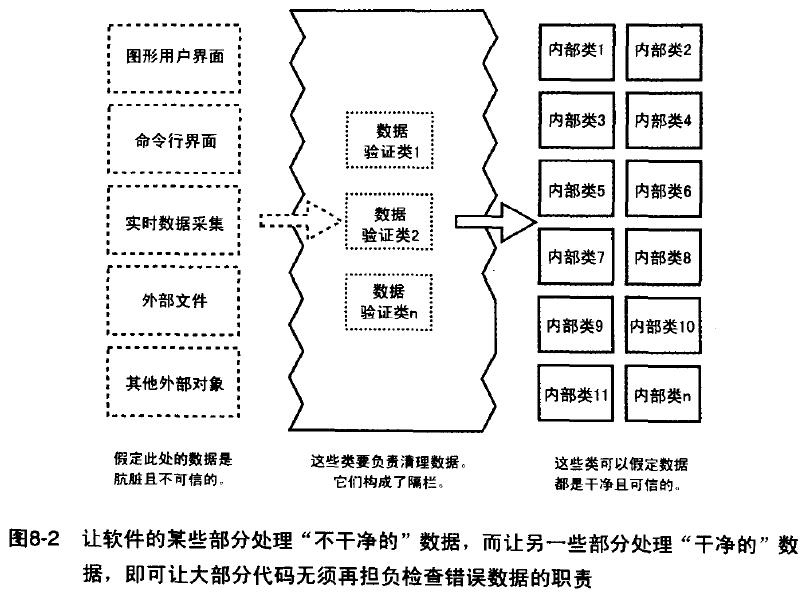
\includegraphics[width=15cm]{figure11.PNG}
\end{figure}
同样地可以在类的层次采用这种方法。类的公用方法可以假设数据是不安全的,它们要负责检查数据并进行清理。一旦类
的公用方法接受了数据,那么类的私用方法就可以假定数据都是安全的了。
\begin{itemize}
    \item 在输入数据时将其转换为恰当的类型:输入的数据通常都是字符串或数字的形式。这些数据有时要被映射为
    “是”或“否”这样的布尔类型,有时要被映射为像Color\_Red、Color\_Green和Color\_Blue这样的枚举类型。在程序
    中长时间传递类型不明的数据,会增加程序的复杂度和崩溃的可能性,比如有人在需要输入颜色枚举值的地方,
    输入了“是”,因此,应该在输入数据后立即将其转换到恰当的类型。
\end{itemize}
\par
隔栏的使用使断言和错误处理,有了清晰的区分。隔栏外部的程序应使用错误处理技术,在那里对数据做的任何假定
都是不安全的。而隔栏内部的程序里,就应使用断言技术,因为传进来的数据应该已通过隔栏时,被清理过了。如果隔栏内部的
某个子程序检测到了错误的数据,那么这应该时程序里的错误,而不是数据里的错误。

\subsection{辅助调试的代码}
防御式编程的另一重要方面是使用辅助调试代码,辅助调试代码非常强大,可以帮助快速地检测错误。
\par
(1)不要自动地把产品版地限制,强加于开发版本之上
\par
应该在开发期间,牺牲一些速度和对资源的使用,来换取一些可以让开发更顺畅的内置工具。
\par
(2)尽早地引入辅助调试的代码
\par
通常,除非被某个错误反复地纠缠,否则你是不愿意花精力,去编写一些调试辅助地代码地;然而,如果你一遇到问题,就马上
编写或使用前一个项目中,用过的某个调试助手的话,它就会自始至终在整个项目中帮助你。
\par
(3)采用进攻式编程
\par
进攻式编程,是指以这样的方式处理异常情况:在开发阶段,让它显现出来,而在产品代码运行时,让它能够自我恢复。
假设有一段case语句,期望用它处理5类事件。在开发期间,应该让针对默认情况的case分支(即default case子句)显示
警告信息;然而,在最终的产品代码里,针对默认情况的处理,则应更稳妥一些,例如可以在错误日志文件中,记录该消息。
下面列出一些可以让你进行进攻式编程的方法:
\begin{itemize}
    \item 确保断言语句使程序终止运行。
    \item 完全填充分配到的所有内存,这样可以让你检测到内存分配错误。
    \item 完全填充已分配到的所有文件或流,这样可以让你排查出文件格式错误。
    \item 确保每一个case语句中的default分支,或else分支,都能产生严重错误,比如说让程序终止,或者至少让
    这些错误不会被忽视。
    \item 在删除一个对象前,把它填满垃圾数据。
    \item 让程序把它的错误日志文件,用电子邮件发给你,这样就能了解到在已发布的软件中,还发生了哪些错误,如果
    这对你所开发的软件适用的话。
\end{itemize}
\par
(4)计划移除调试辅助的代码
\par
事先做好计划,避免调试用的代码,和程序代码纠缠不清。下面使一些可以采用的方法:
\begin{itemize}
    \item 使用类似ant和make这样的版本控制工具和make工具:版本控制工具可以从同一套源码,编译出不同版本的程序。
    在开发模式下,你可以让make工具把所有的调试代码都包含进来一起编译。而在产品模式下,又可以让make工具把那些
    你不希望包含在商用版本中的调试代码排除在外。
    \item 使用内置的预处理器:可以用编译器开关来包含或排除调试用的代码。你既可以直接使用预处理器,也可以写一个
    与预处理器指令同时使用的宏。例如
    \begin{lstlisting}
        C++示例:直接使用预处理器来控制调试用的代码
        #define DEBUG
        ...
        #if defined( DEBUG )
        // debugging code
        ...
        #endif 
    \end{lstlisting}
    如果你不喜欢让\#if defined()这样的语句,散布在代码里的各处,那么可以写一个预处理器宏,来完成同样的任务。例如:
    \begin{lstlisting}
        C++示例:使用预处理器宏,来控制调试用的代码
        #define DEBUG
        #if  defined( DEBUG )
        #define DebugCode( code_fragment ) { code_fragment }
        #else
        #define DebugCode( code_fragment )
        #endif
        ...
        DebugCode(
            statement 1;
            statement 2;
            ...
            statement n;
        );
        ...
    \end{lstlisting}
    \item 编写你自己的预处理器:如果某种语言没有包含一个预处理器,可以很容易自己写一个,用于包含或排除调试代码。
    \item 使用调试存根:很多情况下,可以调用一段子程序进行调试检查。在开发阶段,该子程序可能要执行若干操作之后,
    才把控制权交还给其调用方代码。而在产品代码里,可以用一个存根子程序来替换这个复杂的子程序,而这段stub子程序
    要么立即把控制权交还调用方,要么使执行几项快速的操作就返回。这种方法金辉带来很小的性能损耗,并且比自己编写
    预处理器要快一些。把开发版本和产品版本的stub子程序都保留起来,以便将来可以随时在两者之间来回切换。
    例如,可以先写一个检查出入的指针是否有效的子程序:
    \begin{lstlisting}
        C++示例:一段使用调试stub的子程序
        void DoSomething(
            SOME_TYPE *pointer;
            ...
            ) {
            
            // check parameters passed in
            CheckPointer( pointer )
            ...
        }
    \end{lstlisting}
    在开发阶段,CheckPointer()子程序会对传入的指针,进行全面检查。这一检测可能相当耗时,但一定要非常有效,比如
    这样:
    \begin{lstlisting}
        C++示例:在开发阶段检查指针的子程序
        void CheckPointer( void *pointer ) {
            // 执行第1项检查:可能是检查它不为NULL
            // 执行第2项检查:可能是检查它的地址是合法的
            // 执行第3项检查:可能是检查它所指向的数据完好无损
            ...
            // 执行第n项检查:...
        }
    \end{lstlisting}
    当代码准备妥当,即将要编译为产品时,你可能不希望这项指针检查,影响性能。这是你就可以用下面子程序,来代替前面
    的那段代码:
    \begin{lstlisting}
        C++示例:在产品代码中检查指针的子程序
        void CheckPointer( void *pointer ) {
            // no code; just return to caller
        }
    \end{lstlisting}
\end{itemize}

\subsection{确定在产品代码中该保留多少防御式代码}
下面是一些指导建议,帮助决定哪些防御式编程工具可以留在产品代码里,而哪些应该排除在外:
\begin{itemize}
    \item 保留那些检查重要错误的代码:你需要确定程序的哪些部分,可以承担未检测出错而造成的后果,而哪些部分不能承担;
    \item 去掉检查细微错误的代码:如果一个错误带来的影响确实微乎其微的话,可以把检查它的代码去掉。
    \item 去掉可以导致程序硬件崩溃的代码:如果程序里存在可能导致数据丢失的调试代码,一定要把它们从最终软件产品中去掉。
    \item 保留可以让程序稳妥地崩溃地代码:如果程序里有能够检测出潜在严重错误地调试代码,那么应该保留那些能让
    程序稳妥地崩溃地代码。
    \item 为你地技术支持人员记录错误信息:如果开发时在代码里大量使用了断言来中止程序执行,那么在发布产品时,
    可以考虑把断言子程序改为向日志文件中记录信息,而不是彻底去掉这些代码。
    \item 确认留在代码中的错误信息是友好的:如果你在程序中留下了内部错误消息,请确认这些消息的用语对用户而言
    是友好的。
\end{itemize}

\subsection{对防御式编程采取防御的姿态}
过度的防御式编程也会引起问题。如果你在每一个能想到的地方,用每一种能想到的方法检查从参数传入的数据,那么你的
程序将会变得臃肿而缓慢。更糟糕的是,防御式编程引入的额外代码,增加了软件的复杂度。防御式编程引入的代码也许
并不会有缺陷,和其他代码一样,你同样能轻而易举地,在防御式编程添加地代码中,找到错误,尤其是当你随手编写这些
代码时,更是如此。因此,要考虑好什么地方需要进行防御,然后因地制宜地调整,进行防御式编程地优先级。


\section{伪代码编程过程}
\subsection{创建类和子程序地步骤概述}
创建一个类可以有多种不同的方式,但一般而言,都是一个迭代过程:先对一个类做总体设计,列出这个类内部的特定子程序,
创建这些子程序,然后从整体上复查这个类的构建结果。如下图所示:
\begin{figure}[htb]
    \centering
    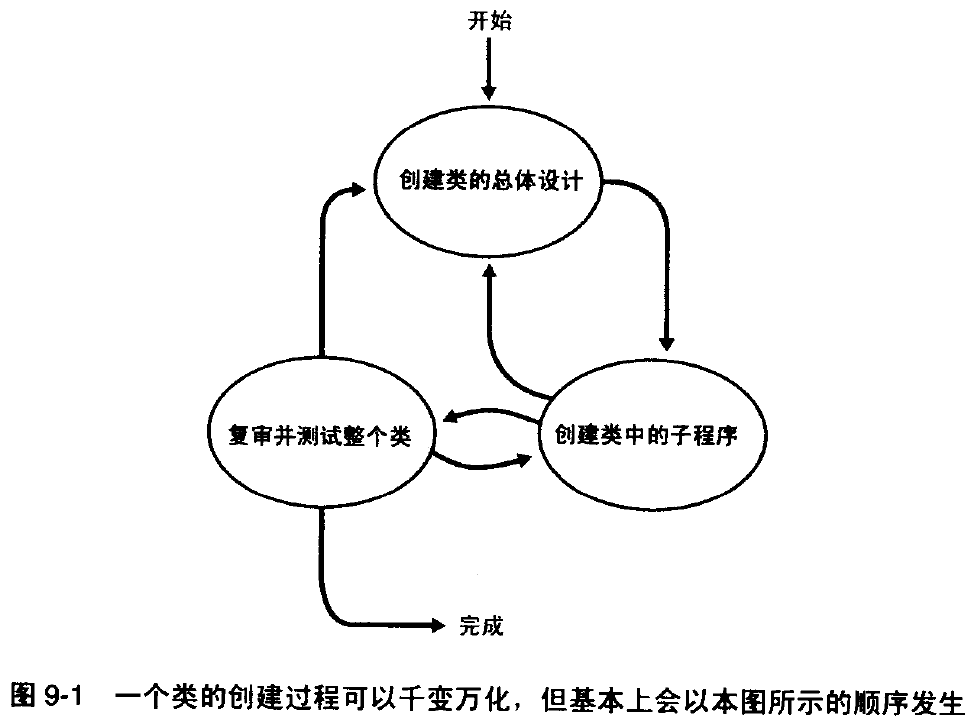
\includegraphics[width=15cm]{figure12.png}
\end{figure}
\par
(1)创建一个类的步骤
\par
\begin{itemize}
    \item 创建类的总体设计:设计一个类的过程中,包含一些特有的设计任务:定义类的特定职责,定义类所要隐藏的
    秘密,以及精确地定义类的接口所代表的抽象概念,决定这个类是否要从其他类派生而来,以及是否允许其他类再从它
    派生,指出这个类中关键的公用方法,标识并设计出类所需用到的重要数据成员。上述这些设计任务可能需要反复迭代,
    直到能直截了当地设计出子程序为止。
    \item 创建类中地子程序:在标识出类的主要子程序后,还要创建这些子程序。在编写各个程序时,通常还会引出更多
    的或重要、或次要的子程序,创建这些新加入的子程序的过程,往往还会反过来波及类的总体设计。
    \item 复审并测试整个类:通常情况下,子程序在创建的同时,也经过了测试。在整个类可以工作之后,应该再对
    其整体进行复查和测试,以便发现那些在子程序的独立测试层次上无法测出的问题。
\end{itemize}

\par
(2)创建子程序的步骤
\par
在创建子程序的过程中,涉及到的主活动:设计子程序、检查设计、编写子程序地代码、检查代码,通常会以下图所示的
顺序进行,
\begin{figure}[htb]
    \centering
    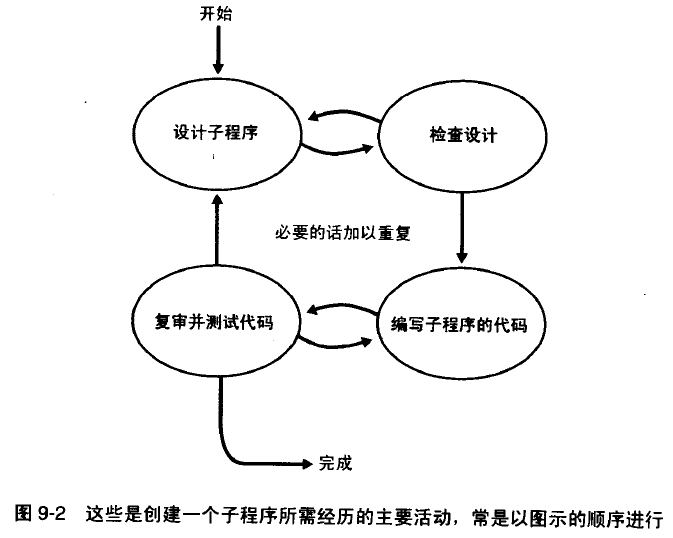
\includegraphics[width=15cm]{figure13.PNG}
\end{figure}

\subsection{伪代码}
伪代码是指某种用来描述算法、子程序、类或完整程序的工作逻辑、非形式的、类似于英语的记法。伪代码编程过程,则是
一种通过书写伪代码而更高效地创建程序代码地专门方法。下面是一些有效使用伪代码地指导原则,
\begin{itemize}
    \item 用类似英语的语句来精确描述特定的操作。
    \item 避免使用目标编程语言中的语法元素。
    \item 在意图的层面上编写伪代码。用伪代码去描述解决问题的方法的意图,而不是去写如何在目标语言中
    实现这个方法。
    \item 在一个足够低的层次上编写伪代码,以便可以近乎自动地从它生成代码。如果伪代码的层次太高,就会
    掩盖代码中的问题细节。应该不断地精细化伪代码,加入越来越多的细节,直到看起来已经很容易直接写出
    代码为止。
\end{itemize}
下面通过例子展示不好的伪代码和好的伪代码:
\begin{lstlisting}
    一段不好的伪代码示例
    increment resource number by 1
    allocate a dlg struct using malloc
    if malloc() returns NULL then return 1
    invoke OSrsrc_init to initialize a resource for the operating system
    *hRsrcPtr = resource number
    return 0
\end{lstlisting}
差的原因:包含许多目标语言编码的细节,例如*hRsrcPtr和malloc()是C语言的特色;这段伪代码太关注于如何编写代码,
而没有突出设计意图;另外它还深入到了编码的细节,即这个子程序是返回1还是0。
\begin{lstlisting}
    一段好的伪代码示例
    Keep track of current number of resource in use
      If another resource is available
        Allocate a dialog box structure
        If a dialog box structure could be allocated
            Note that one more resource is in use
            Initialize the resource
            Store the resource number at the location provided by the caller
        Endif
      Endif
    Return true if a new resource was created; else return false
\end{lstlisting}
使用这种风格的伪代码,可以得到下面这些好处:
\begin{itemize}
    \item 伪代码使得评审更容易。你无须检查源代码就可以评审细节设计。
    \item 伪代码支持反复迭代精细化的思想。从一个高层设计开始,把这一设计精细化为伪代码,然后再把伪代码精细化
    为源代码。
    \item 伪代码使得变更更加容易。短短几行伪代码,要比整页的代码跟容易修改。
    \item 伪代码能使给代码作注释的工作量减到最少。。在伪代码编程过程中,伪代码中的语句,将会变为代码
    中的注释。
    \item 伪代码比其他形式的设计文档更容易维护。使用其他方法时,设计和代码是分离的,当其中之一变动的
    时候,两者就不再一致。而使用伪代码编程过程时,伪代码中的语句将会转变为代码中的注释。因此只要
    维护代码间的这些注释,那么这些伪代码所形成的设计文档就仍然时准确的。
\end{itemize}

\subsection{通过伪代码编程过程创建子程序}
假如你要写一个子程序,它能根据错误码输出错误信息,称它为ReportErrorMessage()。下面是ReportErrorMessage()
程序的一个非形式的规格说明:
ReportErrorMessage()接收一个代表错误码的输入参数,输入与该错误码相对应的错误信息,它应该能够处理无效的
错误码。如果程序是以交互式界面运行的,那么ReportErrorMessage()需要向用户显示错误信息;如果程序是以
命令行方式运行的,那么ReportErrorMessage()应把错误信息记录在一个消息文件里。在输出错误信息之后,
ReportErrorMessage()应返回一个状态值,以表明其操作时成功还是失败。

\par
(1)设计子程序
\par
\begin{itemize}
    \item 检查先决条件:在动手去做子程序本身的任何工作之前,应该先查看一下该子程序要做的工作是不是
    已经定义好了,是不是能够与整体设计相匹配。另外要结合项目的需求,检查这个程序是否时真正必需的,
    至少是间接需要的。
    \item 定义子程序要解决的问题:陈述该子程序将要解决的问题,叙述要足够详细,以便能去创建这个子程序。
    如果高层设计已经足够详细,那么这项工作可能已经完成了。在这个高层的设计里,至少应该详细说明下列信息:
    \begin{itemize}
        \item 这一子程序将要隐藏的信息。
        \item 传给这个子程序的各项输入。
        \item 从该子程序得到的输出。
        \item 在调用程序之前确保有关的前条件成立,如输入数据的取值位于特定的范围之内、有关的流程已经
        初始化、文件已经打开或关闭、缓冲区已经填满或清空等。
    \end{itemize}
    下面看看在ReportErrorMessage()示例中是如何考虑这些问题的:
    \begin{itemize}
        \item 该子程序隐藏了两项事实:错误信息的文本和当前的处理方式,交互式界面或命令行。
        \item 对于这个子程序,没有任何可保证的前条件。
        \item 给该子程序的输入数据是一个错误码。
        \item 存在两种输出:首先是错误信息,其次是ReportErrorMessage()返回给调用方程序的状态值。
        \item 该子程序保证状态值为Success或Failure。
    \end{itemize}
    \item 为子程序命名:一般来说,子程序应该有一个清晰、无歧义的名字。如果你在给程序起个好名字的时候犯难,
    通常就表明这个子程序的目标还没明确。
    \item 决定如何测试子程序:在编写一个子程序的时候,要想一想怎么才能测试它。
    \item 在标准库中搜寻可用的功能:要想提高代码的质量和生产率,一个重要的途径就是重用好的代码。
    \item 考虑错误处理:考虑在子程序中所有可能出错的环节。
    \item 考虑效率问题:根据所确定的资源及速度的目标来设计子程序。如果速度看上去更为重要,
    那么就牺牲一部分资源来换取速度,反之亦然。在每个子程序上为效率问题卖力通常是白费功夫,
    最主要的优化,还是在于完善高层设计,而不是完善每个子程序。
    \item 研究算法和数据类型:在决定从头开始编写一段复杂的代码之前,查一下书法书里有什么可用的内容。
    \item 编写伪代码:在代码编辑工具或集成开发环境里写伪代码就可以了,因为很快就要用这些伪代码
    作为编程语言写的实际编码的基础。从最一般情况写起,向着更具体的细节展开工作。子程序最常见的部分
    是一段头部注释,用于描述这段程序应该做什么,所以首先简要地用一句话来写下该子程序的目的。一般而言,
    如果很难总结出一个子程序的角色,你可能就应该考虑是否什么环节出问题了。下面的例子是描述一个子程序
    的伪代码示例
    \begin{lstlisting}
        一个子程序的伪代码示例
        This routine outputs an error message based on an error code 
        supplied by the calling routine. The way it outputs the message 
        depends on the current processing state, which it retrievess
        on its own. It returns a value indicating success or failure.

        set the default statues to "fail"
        look up the message based on the error code
        if the error code is valid
            if doing interactive processing, display the error message
            interactively and declare success
            if doing command line processing, log the error message to the 
            command line and declare success
        if the error code isn't valid, notify the user that an internal 
        error has been detected.
        return status information
    \end{lstlisting}
    \item 考虑数据:如果对数据的操作是某个子程序的重点,那么值得在考虑子程序的逻辑之前,首先考虑主要的
    数据部分。把关键的数据类型定义好,对于设计一个子程序的逻辑很有用。
    \item 检查伪代码:请确认你能很容易、很自然地理解这个子程序做些什么,以及它是怎样做地。、
    \item 在伪代码中试验一些想法,留下最好的想法(迭代):在你开始编写代码之前,应尽可能用伪代码去尝试
    更多的想法。一旦你真正开始编码,你和你所写下的代码就会有感情,从而更难以抛弃不好的设计再重头来过了。
\end{itemize}


\par
(2)编写子程序的代码
\par
构建子程的步骤如下,
\begin{figure}
    \centering
    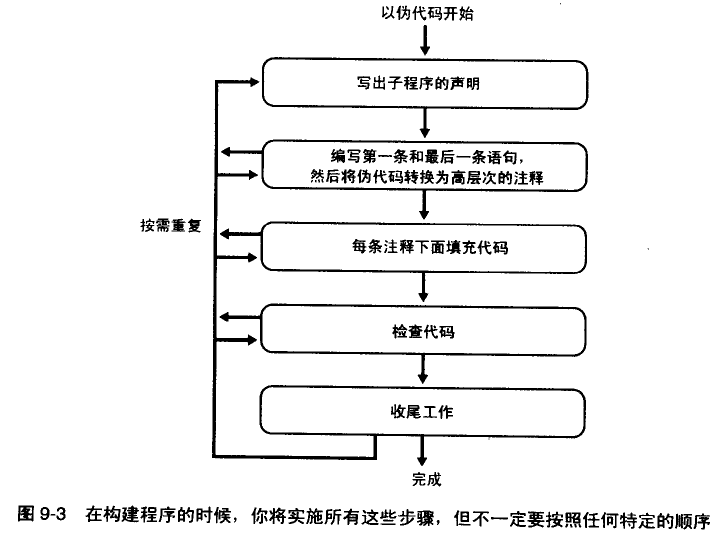
\includegraphics[width=15cm]{figure14.PNG}
\end{figure}
\begin{itemize}
    \item 写出子程序的声明:首先写出子程序的接口声明,例如C++中的函数声明。把原有的头部注释变为编程语言中
    的注释。把它保留在你写的伪代码的上方。
    \begin{lstlisting}
        C++示例:向伪代码添加子程序接口声明和头部注释
        /* This routine outputs an error message based on an error code 
        supplied by the calling routine. The way it outputs the message 
        depends on the current processing state, which it retrievess
        on its own. It returns a value indicating success or failure.
        */

        Status ReportErrorMessage(
            ErrorCode errorToReport
        )
        set the default statues to "fail"
        look up the message based on the error code
        if the error code is valid
            if doing interactive processing, display the error message
            interactively and declare success
            if doing command line processing, log the error message to the 
            command line and declare success
        if the error code isn't valid, notify the user that an internal 
        error has been detected.
        return status information
    \end{lstlisting}
    \item 把伪代码转变为高层次的注释:接下来,把第一条和最后一条语句写出来,在C++中也就是“\{”和"\}"。然后
    把伪代码转变为注释。
    \begin{lstlisting}
        C++示例:在伪代码首尾写出第一条和最后一条语句
        /* This routine outputs an error message based on an error code 
        supplied by the calling routine. The way it outputs the message 
        depends on the current processing state, which it retrievess
        on its own. It returns a value indicating success or failure.
        */

        Status ReportErrorMessage(
            ErrorCode errorToReport
        ) {
            //set the default statues to "fail"
            //look up the message based on the error code
            //if the error code is valid
                //if doing interactive processing, display the error message
                //interactively and declare success
                //if doing command line processing, log the error message to the 
                //command line and declare success
            //if the error code isn't valid, notify the user that an internal 
            //error has been detected.
            //return status information
        }
    \end{lstlisting}
    \item 在每条注释下面填充代码:每一段注释产生出一行或多行代码。以这些注释为基础,每一代码块都形成了一套
    完整的思想。这些注释仍然保留下来,从一个更高的层次上对代码做出说明。所有的变量都是在靠近第一次使用的
    地方来进行声明和定义。每段注释通常应该展开为2至10行代码。
    \begin{lstlisting}
        C++示例:在伪代码首尾写出第一条和最后一条语句
        /* This routine outputs an error message based on an error code 
        supplied by the calling routine. The way it outputs the message 
        depends on the current processing state, which it retrievess
        on its own. It returns a value indicating success or failure.
        */

        Status ReportErrorMessage(
            ErrorCode errorToReport
        ) {
            //set the default statues to "fail"
            Status errorMessageStatus = Status_Failure;

            //look up the message based on the error code
            Message errorMessage = LookupErrorMessage( errorToReport );

            //if the error code is valid
            if ( errorMessage.ValidCode() ) {
                // determine the processing method
                ProcessingMethod errorProcessingMethod = 
                    CurrentProcessingMethod();

                //if doing interactive processing, display the error message
                //interactively and declare success
                if ( errorProcessingMethod == ProcessingMethod_Interactive ) {
                    DisplayInteractiveMessage( errorMessage.Text() );
                    errorMessageStatus = Status_Success;
                }

                //if doing command line processing, log the error message to the 
                //command line and declare success
                else if ( errorProcessingMethod ==
                    ProcessingMethod_CommanLine ) {
                        CommandLine messageLog;
                        if ( messageLog.Status() == CommondLineStatus_OK ) {
                            messageLog.AddToMessageQueue( errorMessage.Text() );
                            messageLog.FlushMessageQueue();
                            errorMessageStatus = Status_Success;
                        } else {
                            // can't do anything because the routine is already
                            // error processing
                        }
                    } else {
                        // can't do anything because the routine is already
                        // error processing
                    }
            }
            //if the error code isn't valid, notify the user that an internal 
            //error has been detected.

            else {
                DisplayInteractiveMessage(
                    "Internal Error: Invalid error code in ReportErrorMessage()"
                );
            }

            //return status information
            return errorMessageStatus;
        }
    \end{lstlisting}
    \item 检查代码是否需要进一步分解:有时候,你会发现几行伪代码展开后,形成大量的代码。在这种情况下,应该
    考虑如下两种方法中的一种:
    \begin{itemize}
        \item 把这段注释下的代码重构成一个新的子程序。
        \item 递归地应用伪代码编程过程。把原来的那一行伪代码分解为更多行的伪代码,然后再在新写出的伪代码下面
        填入代码。
    \end{itemize}
\end{itemize}

\par
(3)检查代码
\par
\begin{itemize}
    \item 在脑海中检查程序中的错误:在脑海中执行每一条代码路径,确保检查到了所有可能的执行路径、端点和所有
    异常条件。底线:只是写出一个可以工作的子程序是不够的,如果你不知道它为什么可以工作,那就去研究它,讨论它,
    用其他的设计方案做试验,直到你弄明白为止。
    \item 编译子程序:本书的一个目的就是告诉你,怎样脱离那种先东拼西凑,然后通过运行来看看代码是否工作的
    怪圈,不要挣扎于“拼凑、编译、修改”的开发工作中。下面一些指导建议,可以最大限度地发挥编译子程序所产生的
    功效:
    \begin{itemize}
        \item 把编译器的警告级别调到最高,让编译器来检测错误,可以很容易地查出大量细微的错误。
        \item 使用验证工具。可以通过使用类似lint这样的工具,对C语言这类语言的编译器所作的检查结果,进行补充检查。
        \item 消除产生错误消息和警告的所有根源。通常,大量的告警信息暗示着代码的质量欠佳,你需要尽量理解所
        得到的每一个告警。通过重写代码来解决潜在问题并消除告警信息,是更保险也更省力的。
    \end{itemize}
    \item 在调试器中逐行执行代码。
    \item 测试代码。使用你在开发该子程序期间,计划写的或已写成的测试用例,来测试代码。
    \item 消除程序中的错误。一旦检测到错误,就一定要把它除掉。如果你发现一段程序的毛病不是一般的多,那请、
    从头再来吧。修修补补通常表明你还未能全面地理解程序,这样也必将不时地产生错误。对于一个毛病百出的程序
    而言,设计一个全新的方案是值得的。
\end{itemize}

\par
(4)收尾工作
\par
可以实行若干扫尾步骤来确保子程序的质量合乎标准:
\begin{itemize}
    \item 检查子程序的接口。确认所有的输入、输出数据都参与了计算,并且所有的参数也都用到了。
    \item 检查整体的设计质量。确认下列事项:这个子程序只干一件事情,并且把这件事情做得很好;子程序之间是
    松散耦合的;子程序采用了防御式设计。
    \item 检查子程序中的变量。检查是否存在不准确的变量名称、未被用到的对象、未经声明的变量,以及未经正确
    初始化的对象等。
    \item 检查子程序的语句和逻辑。检查是否存在off-by-one这样的错误、死循环、错误的嵌套以及资源泄露。
    \item 检查子程序的布局。确认你正确地使用了空白来明确子程序、表达式及参数列表的逻辑结构。
    \item 检查子程序的文档。确认哪些由伪代码转化而来的注释,仍然是准确无误的。检查有关算法的描述、接口假定
    的说明、那些并非显而易见的依赖性,以及难以理解的编码行为的解释等。
    \item 除去冗余的注释。
\end{itemize}

\par
(5)根据需要重复上述步骤
\par
如果这个程序的质量不佳,那就回到伪代码那一步去。高质量的编程是一个迭代的过程,所以不要犹豫,把构建的工作
再做一遍。

\section{使用变量的一般事项}
本章中用“变量”一词同时指代对象和内置数据类型,如整数和数组等。“数据类型”一词通常是
内置数据类型,而“数据”一词则可能代表对象,也可能代表内置数据类型。
\subsection{数据认知}
创建有效数据的第一步是了解所要创建数据的种类。积累大量的数据类型,对于程序员来说是至关重要的。

\subsection{轻松掌握变量定义}
养成一个良好的变量定义习惯,会为你再整个项目周期内,省去很多时间和麻烦。有些语言支持隐式变量声明。
例如Microsoft Visual Basic中使用一个未申明变量的时候,编译器会自动为你声明该变量。隐式变量声明对于任何一种语言
来说,都是最具危险性的特性之一。例如,当你绞尽脑汁想要明白变量acctNo的值为什么不正确,最终却发现是不慎将
acctNo写成acctNum,而又将acctNum重新初始化为0。要求显示声明数据的编程语言,实际上是在提醒你要更加仔细地使用
这些数据,而这一点也是它们的主要优势之一。如果使用的编程语言支持隐式声明,下面是一些建议:
\begin{itemize}
    \item 关闭隐式声明。
    \item 声明全部变量。
    \item 遵循某种命名规则。
    \item 检查变量名。
\end{itemize}

\subsection{变量初始化原则}
不合理地初始化数据是产生编程错误地常见根源之一。不恰当地变量初始化所导致的一系列问题,都源于变量的默认初始化值,
与你的预期不同。以下行为都会产生此类问题:
\begin{itemize}
    \item 从未对变量赋值。它的值只是程序启动时,变量所处内存区域的值。
    \item 变量值已经过期。变量在某个地方曾经被赋值,但该值已经不再有效。
    \item 变量的一部分被赋值,而另一部分没有。你可能初始化了一个对象的部分成员,而不是全部成员。也可能忘记
    事先分配内存,就去初始化一个未经初始化的指针所指的“变量”。这就意味着你是随机选取了一块内存,然后对其赋值。
    这块内存可能存放的是数据,也可能存放的是代码,甚至可能指向操作系统内部。指针操作错误可能产生很奇怪的现象,
    并且每次都不相同,这也导致了调试指针错误,比调试其他错误更困难。
\end{itemize}
下面是一些避免产生初始化错误的建议:
\begin{itemize}
    \item 在声明变量的时候初始化:在声明变量的同时对其初始化,是一种非常方便的防御式编程方法,是一种很好的
    用于防范初始化错误的保险策略。
    \item 在靠近变量第一次使用的位置初始化它:这是就近原则的一个例子,即把相关的操作放在一起。这一原则也适用
    于让注释靠近它所描述的代码,让控制循环的代码靠近循环本身,以及把语句写成直线的代码等各个领域。
    \item 理想情况下,在靠近第一次使用变量的位置声明和定义该变量:声明指定了变量的类型,定义为变量指定特定的取值。
    在理想情况下,每个变量都应该在声明的同时被定义。
    \item 在可能的情况下使用final或const:可以防止该变量在初始化后,再被赋值。
    \item 特别注意计数器和累加器:i、j、k、sum和total等变量常用作计数器或累加器,在下次使用这些变量之前,忘记
    重置其值,也是一种常见的错误。
    \item 在类的构造函数里初始化该类的数据成员:类的数据也应该在其构造函数中初始化,如果在构造函数里分配了内存,
    那么就应该在析构函数中释放这些内存。
    \item 检查是否需要重新初始化:如果的确需要重新初始化,那么要确保初始化语句位于那些重复执行的代码内部。
    \item 一次性初始化具名常量,用可执行代码来初始化变量:如果你想用变量来模拟具名常量,那么在程序开始处
    对常量做一次初始化即可。你可以用一个Startup()子程序去初始化它们。
    \item 使用编译器设置来自动化初始化所有变量:如果你用的编译器支持自动化初始化所有变量的选项,那么请把它打开。
    这是一种靠编译器完成初始化工作的简单方式。然而,跨平台移植,则会带来问题。因此要确保记下你所使用的编译器设置。
    \item 利用编译器的告警信息:很多编译器会在你使用了未经初始化的变量的时候发出警告。
    \item 检查输入参数的合法性:在你把输入数值赋给任何对象之前,要确保这些数值是合理的。
    \item 使用内存访问检查工具来检查错误的指针。
    \item 在程序开始时初始化工作内存:把工作内存初始化为一个已知数值,将会有助于发现初始化错误。可以采用下面的
    任意一种方法,
    \begin{itemize}
        \item 可以用某种在程序运行前预先填充内存的工具,来把程序的工作内存填充为一个可以预料的值。
        \item 如果使用内存填充工具,那么可以偶尔改变一下用来填充的内存的值。有时,这么“晃动”一下程序,也许可以
        发现一些在在背景环境保持不变的情况下,无法察觉出来的错误。
        \item 可以让程序在启动时初始化工作内存。前面所述的使用在程序运行时,预先填充内存的工具的目的,是要暴露
        缺陷,而这种方法的目的,则是隐藏缺陷。通过每次把工作内存赋以同样的值,就能保证程序不会因内存初始值的
        随机性而受到影响。
    \end{itemize}
\end{itemize}

\subsection{作用域}
作用域或可见性指的是变量在程序内的可见和可引用的范围。下面是一些使用作用域的规则:
\par
(1)使变量引用局部化
\par
那些介于同一变量多个引用点之间的代码,成为“攻击窗口”。可能会由新代码加到这种窗口中,不当地修改了这个变量,
或者阅读代码地人,可能会忘记该变量应有地值。一般而言,把对一个变量的引用局部化,即把引用点尽可能集中在
一起,总是一种很好的做法。衡量一个变量的不同引用点的靠近程度的一种方法,是计算该变量的“跨度(span)”。例如,
\begin{lstlisting}
    Java示例:变量跨度
    a = 0;
    b = 0;
    c = 0;
    b = a + 1;
    b = b / c;
\end{lstlisting}
其中a的跨度为2,b的跨度为1和0,平均跨度为0.5,c的跨度为1。如果这些引用点之间的距离非常远,那你就要迫使
阅读者的目光在程序里跳来跳去。因此,把变量的引用点集中起来的主要好处,是提高程序的可读性。
\par
(2)尽可能缩短变量的存活时间
\par
与变量跨度相关的一个概念是“存活时间”,即一个变量存在期间,所跨越的语句总数。变量的存活时间,开始于引用它的第一天语句,
结束于引用它的最后一条语句。与跨度类似,应使得对象的存活时间尽可能短,保持短的存活时间的主要好处,也是减小
攻击窗口。这样,在你真正想要修改一个变量的那些位置之间的区域,该变量被错误或无意修改的可能性就降低了。
短的变量存活时间同样减少了初始化错误的可能。在修改程序的时候,常会把直线型代码(顺序代码)修改为循环,这样
就容易忘记远离循环位置的那些初始化代码。通过把初始化代码和循环代码放在一起,就减少了由于修改语句,而导致
初始化错误的可能性。变量存活时间还会使代码更具有可读性。阅读者在同一时间内,需要考虑的代码行数越少,也就越容易
理解代码。最后,当需要把一个大的子程序拆分为多个小的子程序时,短的变量存活时间也是有价值的。如果你用跨度和
生存时间的概念来考虑全局变量,就会发现全局变量的跨度和生存时间都很长,这也是避免使用全局变量的好理由之一。
\par
(3)减小作用域的一般原则
\par
\begin{itemize}
    \item 在循环开始之前,再去初始化该循环里使用的变量,而不是在该循环所属的子程序的开始处,初始化这些变量。
    \item 直到变量即将被使用时,再为其赋值。
    \item 把相关语句放到一起。
    \begin{lstlisting}
        C++示例:使用两套变量,使人困惑的做法
        void SummarizeData(...) {
            ...
            GetOldData( oldData, &numOldData );
            GetNewData( newData, &numNewData );
            totalOldData = Sum( oldData, numOldData );
            totalNewData = Sum ( newData, numNewData );
            PrintOldDataSummary( oldData, totalOldData, numOldData );
            PrintNewDataSummary( newData, totalNewData, numNewData );
            SaveOldDataSummary( totalOldData, numOldData );
            SaveNewDataSummary( totalNewData, numNewData );
            ...
        }
    \end{lstlisting}
    \begin{lstlisting}
        C++示例:使用两套变量,更容易理解的做法
        void SummarizeData(...) {
            GetOldData( oldData, &numOldData );
            totalOldData = Sum( oldData, numOldData );
            PrintOldDataSummary( oldData, totalOldData, numOldData );
            SaveOldDataSummary( totalOldData, numOldData );
            ...
            GetNewData( newData, &numNewData );
            totalNewData = Sum ( newData, numNewData );
            PrintNewDataSummary( newData, totalNewData, numNewData );
            SaveNewDataSummary( totalNewData, numNewData );
            ...
        }
    \end{lstlisting}
    \item 把相关语句组提取成单独子程序。在其他相同的情况下,一个更短的子程序中的变量,通常比更长的子程序中
    的变量,有更小的跨度和存活时间。
    \item 开始时采用最严的可见性,然后根据需要,扩展变量的作用域。当对变量的作用域犹豫不决时,应该倾向于选择
    该变量所能具有的最小的作用域:首先将变量局限于某个特定的循环,然后局限于某个子程序,其次成为类的private
    变量,protected变量,再其次对package可见,最后不得已的情况下,在把它作为全局变量。
\end{itemize}

\subsection{持续性}
“持续性”是对一项数据的生命周期的另一种描述。持续性具有多种形态:
\begin{itemize}
    \item 特定代码段或子程序的生命周期。例如在C++或Java中的for循环里,声明的变量。
    \item 只要你允许,就会持续下去。例如C++里用new创建的变量,会一直持续到delete它。
    \item 程序的生命期。大多数语言的全局变量,都属于这一类,C++中的static变量也是如此。
    \item 永远持续。这一类变量可能包括你存储在数据库中、能够在程序的多处执行之间存留的数据。
\end{itemize}
与持久性相关的主要问题,是变量实际生命周期比想象的要短,而且难以预料。如果你试图在一个变量正常的生命周期
结束之后,访问它的数据,那么它的数值还会保持吗?有的时候变量中保持的数值已经改变了,你通过收到错误提示
获知这一点。而有时,计算机会把旧的数值留在变量里,使你误认为自己用对了变量。为了避免上述问题,可以采取以下措施:
\begin{itemize}
    \item 在程序中加入调试代码或断言,来检查那些关键变量的合理取值。如果变量取值变得不合理,就发出警告信息,
    通知你去寻找是否有不正确的初始化。
    \item 准备抛弃变量时,给它们赋上“不合理的数值”,例如,可以在删除一个指针后,把它的值设为null。
    \item 编写代码时,要假设数据并没有持续性。例如,如果某个变量在你退出某个子程序的时候,具有特定的值,那么当你
    当你下一次进入该子程序的时候,就不要假定该变量还有同样的数值。
    \item 养成在使用所有数据之前,声明和初始化的习惯。如果你发现某项数据的使用位置与初始化位置相去甚远,那么就要小心了。
\end{itemize}

\subsection{绑定时间}
对程序维护和更改,有很深远影响的一个话题,就是“绑定事件”:把变量和它的值绑定在一起的时间。
采用越晚的绑定时间会越有利。
\begin{lstlisting}
    Java示例:在编写代码时绑定其值的变量
    titleBar.color = 0xFF; // 0xFF is hex value for color blue
\end{lstlisting}
由于0xFF是硬编码在程序里的数值,在编写代码时,它就会绑定到title.color变量上。这种硬编码技术通常总是很糟糕的,
因为一旦要修改这个0xFF,那么这个新值就无法同代码中其他那些必须和它一样的0XFF值保持一致了。
\begin{lstlisting}
    Java示例:在编译时绑定其值的变量
    private static final int COLOR_BLUE = 0xFF;
    private static final int TITLE_BAR_COLOR = COLOR_BLUE;
    ...
    titleBar.color = TITLE_BAR_COLOR;
\end{lstlisting}
TITLE\_BAR\_COLOR是一个具名常量,编译器会在编译的时候,把它替换为一个数值。如果你用的语言支持这种特性,那么这种
方法几乎总要好于硬编码。由于TITLE\_BAR\_COLOR比0xFF更能反映出所代表的信息,因此增加了可读性。它也使得修改标题颜色
变得更容易,因为一处改动就能对所有位置生效。同时也不会影响运行期的性能。
\begin{lstlisting}
    Java示例:在运行时绑定其值的变量
    titleBar.color = ReadTitleBarColor();
\end{lstlisting}
与硬编码相比,上述代码更具可读性和灵活性。无须通过修改程序来改变titleBar.color,只需简单修改ReadTitleBarColor()
子程序要读取的数据源内容即可。这种方法常用于允许用户自定义应用程序环境的交互式应用程序。
\par
一般而言,绑定时间越早,灵活性就会越差,但复杂度也会降低。就前两种方案而言,使用具名常量,要在很多方面好于
使用魔鬼数字(magic number)。

\subsection{数据类型和控制结构之间的关系}
有三种类型的数据和相应控制结构之间的关系:
\begin{itemize}
    \item 序列数据翻译为程序中的顺序语句。
    \item 选择型数据翻译为程序中的if和case语句。
    \item 迭代型数据翻译为程序中的for、repeat、while等循环结构。
\end{itemize}

\subsection{为变量指定单一用途}
\begin{itemize}
    \item 每个变量只用于单一用途。下面例子显示了一个用于两种用途的临时变量:
    \begin{lstlisting}
        C++示例:同一变量用于两种用途,糟糕的实践
        // Compute roots of a quadratic equation
        // This code assume that (b*b-4*a*c) is positive.
        temp = Sqrt( b*b-4*a*c );
        root[0] = ( -b + temp ) / ( 2 * a );
        root[1] = ( -b - temp ) / ( 2 * a );
        ...
        // swap the roots
        temp = root[0];
        root[0] = root[1];
        root[1] = temp;
    \end{lstlisting}
    \begin{lstlisting}
        C++示例:同一变量用于两种用途,糟糕的实践
        // Compute roots of a quadratic equation
        // This code assume that (b*b-4*a*c) is positive.
        discriminant = Sqrt( b*b-4*a*c );
        root[0] = ( -b + discriminant ) / ( 2 * a );
        root[1] = ( -b - discriminant ) / ( 2 * a );
        ...
        // swap the roots
        oldRoot = root[0];
        root[0] = root[1];
        root[1] = oldRoot;
    \end{lstlisting}
    \item 避免让代码具有隐含含义。把同一变量用于多个用途的另一种方式,是当变量代表不同事物时,让其具有不同的取值集合。
    例如:变量pageCount的取值可能表示已打印纸张的数量,除非它等于-1,在这种情况下,表明有错误发生。
    \item 确保使用了所有已声明的变量。与同一变量多种用途相反的,是声明了变量,却不使用。
\end{itemize}

\section{变量名的力量}
\subsection{选择好变量名的注意事项}
\par
(1)最重要的命名注意事项
\par
为变量命名时,最重要的考虑事项是,该名字要完全、准确地描述出该变量所代表的事物。获得好名字的一种实用技巧,
就是用文字表达变量所代表的是什么。通常,对变量的描述,就是最佳的变量名。这种名字很容易阅读,因为其中并不
包含晦涩的缩写,同时也没有歧义。因为它是对该事物的完整描述,因此不会和其他事物混淆。另外,由于这一名字所表达的
概念相似,因此也很容易记忆。

\par
(2) 以问题为导向
\par
一个好记的名字,反映的通常都是问题,而不是解决方案。一般而言,如果一个名字反映了计算的某些方面,而不是问题
本身,那么它反映的就是“how”,而非“what”了。请避免取这样的名字,而应该在名字中反映出问题本身。例如,一条员工
数据记录,可以称作inputRec或employeeData;inputRec是一个反映输入、记录这些计算概念的计算机术语;employData
则指问题领域,与计算的世界无关,因此应该用employeeData。

\par
(3) 最适当的名字长度
\par
太短的名字无法传达足够的信息;太长的名字很难写,同时也会使程序的视觉结构变得模糊不清。研究发现,当变量名的
平均长度在10到16个字符时,调试程序所需花费的力气是最小的。例如numberOfPeopleOnTheUsOlympicTeam太长、
ntm太短、numTeamMembers正好。

\par
(4) 变量名对作用域的影响
\par
短的变量名,有时也是可以的。例如i,这一长度本身就对该变量做出了一些说明,也就是说,该变量代表的是
一个临时的数据,它的作用域非常有限。较长的名字适用于很少用到的变量或全局变量,而较短的名字则适用于局部
变量或循环变量。不过短的变量名常常会带来一些麻烦,因此,作为一项防御式编程策略,应避免使用短的变量名。

\par
(5)变量名中的计算值限定词
\par
很多程序都有表示计算结果的变量:总额、平均值、最大值等等。如果用类似于Total、Sum、Average这样
的限定词来修改这个名字,那么请记住把限定词加到名字的最后。这种方法具有很多优点。首先,变量名中
最重要的那部分,即为这一变量赋予主要含义的那部分应当位于最前面,这样,这一部分就可以显得最为突出,
并会被首先阅读到。其次,采纳了这一规则,你将避免由于同时在程序中使用totalRevenue和revenueTotal而
产生歧义。总之,一致性可以提高可读性,简化维护工作。把计算的量放在名字最后也有例外,那就是Num限定词
的位置已经约定俗成。Num放在变量名的开始位置代表一个总数:numCustomers表示员工总数。Num放在变量名
的结束位置代表一个下标:customerNum表示当前员工的序号。通过numCustomers最后代表复数的s也能够看出这
两种应用之间的叙别。然而,由于这样使用Num常常会带来麻烦,因此可能最好的办法是避开这些问题,用Count
或者Total来代表员工的总数,用Index来指代某个特定的员工。这样,customerCount就代表员工的总数,
customerIndex代表某个特定的员工。

\par
(6)变量名中的常用对仗词
\par
对仗词的使用要准确。通过应用命名规则来提高对仗词使用的一致性,从而提高其可读性。比如像begin/end
这样的一组用词非常容易理解和记忆。

\subsection{为特定类型的数据命名}
(1)循环下标命名
\par
i、j和k这些名字都是约定俗成的:
\begin{lstlisting}
    Java示例:简单的循环变量命名
    for( i = firtstItem; i < lastItem; i++){
        data[i] = 0;
    }
\end{lstlisting}
如果一个变量要在循环之外使用,那么就应该为它取一个比i、j或k更有意义的名字。如果循环不是只有几行,那么
读者会很容易忘记i本来具有的含义,因此你最好给循环下标换一个更有意义的名字。由于代码会经常修改、扩充,
或者复制到其他程序中去,因此,很多有经验的程序员索性不使用类似于i这样的名字。
\begin{lstlisting}
    Java示例:嵌套循环中的好循环变量名
    for( teamIndex = 0; teamIndex < teamCount; teamIndex++ ){
        for( eventIndex = 0; eventIndex < eventCount[teamIndex]; eventIndex++){
            score[teamIndex][eventIndex] = 0;
        }
    }
\end{lstlisting}

\par
(2)状态变量命名
\par
为状态变量取一个比flag更好的名字:状态变量的名字中,不应该含有flag,因为你丝毫看不出该状态变量是做什么的。
为了清楚起见,状态变量应该用枚举类型、具名常量,或用作用具名常量的全局变量来对其赋值,而且其值应该与
上面这些量做比较。
\begin{lstlisting}
    C++示例:含义模糊的标记
    if (flag) ...
    if (statusFlag & 0x0F) ...
    if (printFlag == 16) ...
    if (computeFlag == 0) ...

    flag = 0x1;
    statusFlag = 0x80;
    printFlag = 16;
    computeFlag = 0;
\end{lstlisting}
\begin{lstlisting}
    C++示例:更好地使用状态变量
    if (dataReady) ...
    if (characterType & PRINTABLE_CHAR) ...
    if (reportType == ReportType_Annual) ...
    if (recalNeeded == false) ...

    dataReady = true;
    characterType = CONTROL_CHARACTER;
    reportType = ReportType_Annual;
    recalcNeeded = false;
\end{lstlisting}
下面例子展示了如何使用具名常量和枚举类型来组织例子中地数值:
\begin{lstlisting}
    在C++中声明状态变量
    \\ value for CharacterType
    const int LETTER = 0x01;
    const int DIGIT = 0x12;
    const int PUNCTUATION = 0x04;
    const int LINE_DRAN = 0x08;
    const int PRINTABLE = (LETTER | DIGIT | PUNCTUATION | LINE_DRAW);
    cont int CONTROL_CHARACTER = 0x80;

    \\ values for ReportType
    enum ReportType {
        ReportType_Daily,
        ReportType_Monthly,
        ReportType_Quarterly,
        ReportType_Annual,
        ReportType_All
    };
\end{lstlisting}

\par
(3) 临时变量命名
\par
临时性地保存一些值常常是很有必要的,但是无论从哪种角度看,程序中的大多数变量都是临时性的。把其中几个称为
临时的,可能表明你还没弄清它们的实际用途,例如:
\begin{lstlisting}
    C++示例:不提供信息的临时变量
    \\ Compute roots of a quadratic equation.
    \\ This assumes that (b^2-4*a*c) is positive.
    temp = sqrt(b^2-4*a*c);
    root[0] = (-b + temp) / (2*a);
    root[1] = (-b - temp) / (2*a);
\end{lstlisting}
其中temp没有反映该变量的功能,下面例子展示了一种更好的做法:
\begin{lstlisting}
    C++示例:用真正的变量替代临时变量
    \\ This assume that (b^2-4*a*c) is positive.
    discriminant = sqrt(b^2-4*a*c);
    root[0] = (-b + discriminant) / (2*a);
    root[1] = (-b - discriminant) / (2*a);
\end{lstlisting}

\par
(4) 布尔变量命名
\par
为布尔变量命名时要遵循的几条原则:
\begin{itemize}
    \item 谨记典型的布尔变量名:下面是一些格外有用的布尔变量名,
    \begin{itemize}
        \item done:用done表示某件事情已经完成。这一变量可用于表示循环结束或一些其他的操作已完成。在事情
        完成之前把done设为false,在事情完成之后设为true。
        \item error:用error表示错误发生。在错误发生前设为false,错误发生时设为true。
        \item found:表明某个值已经找到。false->true
        \item success或OK:表明一项操作是否成功。操作失败时为false,成功为true。
    \end{itemize}
    \item 给布尔变量赋予隐含“真/假”含义的名字:像done和success这样的名字是很不错的布尔变量名,因为其状态要么是
    true,要么是false;另一方面,像status和sourceFile这样的名字,就是很糟的布尔变量名,因为它们没有明确
    的true或false状态。
    \item 使用肯定的布尔变量名:否定的名字如notFound、notDone以及notSuccessful等较难阅读,特别是它们被
    求反:if not notFound。
\end{itemize}

\par
(5) 为枚举类型命名
\par
在使用枚举类型的时候,可以通过使用前缀,如Color\_来明确表示该类型的成员都同属于一个组。
例如:
\begin{lstlisting}
    Visual Basic示例:为枚举类型采用前缀命名约定
    Public Enum Color
        Color_Red
        Color_Green
        Color_Blue
    End Enum
\end{lstlisting}
在有些编程语言里,枚举类型的处理和类很像,枚举成员也总是被冠以枚举名字前缀,例如Color.Color\_Red,
那么重复上述前缀的意义就不大了,可以简化为Color.Red。

\par
(6) 为常量命名
\par
为具名常量命名时,应该根据该常量所表示的含义,而不是该常量所具有的数值,为该抽象事物命名。例如,
FIVE就是个很糟的常量命,CYCLES\_NEEDED是个不错的名字。

\subsection{命名规则的力量}
\par
(1) 为什么要有规则
\par
规则的存在为你的代码增加了结构,减少了你需要考虑的事情。命名规则可以带来以下好处:
\begin{itemize}
    \item 可以集中关注代码更重要的特征。
    \item 有助于在项目之间传递知识。
    \item 有助于在新项目中,更快速地学习代码。
    \item 有助于减少名字增生。在没有命名规则的情况下,会很容易给同一个对象起两个不同的名字。例如,
    pointTotal->totalPoints。
    \item 弥补编程语言的不足之处。可以用规则来仿效具名常量和枚举类型。规则可以根据局部数据、类数据
    以及全局数据的不同,而有所差别,并且可以包含编译器不直接提供的类型信息。
    \item 强调相关变量之间的关系。如果编程语言不支持对象,可以用命名规则来予以补充。例如,address、
    phone以及name这样的名字,并不能表明这些变量是否相关;但employeeAddress、employeePhone和
    employeeName就会毫无疑问地表明这些变量时彼此相关的。
\end{itemize}



\section{基本数据类型}

\section{不常见的数据类型}

\section{组织直线型代码}

\section{条件语句}

\section{控制循环}

\section{不常见的控制结构}

\section{表驱动法}

\section{一般控制问题}

\section{软件质量概述}

\section{协同构建}

\section{开发者测试}

\section{调试}

\section{重构}

\section{代码调整策略}

\section{代码调整技术}

\section{程序规模对构建的影响}

\section{管理构建}

\section{集成}

\section{编程工具}

\section{布局与风格}

\section{自说明代码}

\section{个人性格}

\section{软件工艺}

\section{更多信息}


\begin{thebibliography}{99}  
    \bibitem{Meyer2000}Meyer CD (2000) Matrix Analysis and Applied Linear Algebra. Philadelphia, PA: SIAM.
    \bibitem{consistency} Agostino Martinelli. Closed-form solution of visual-inertial structure from motion. International
    Journal of Computer Vision, Springer Verlag, 2013. ￿hal-00905881
\end{thebibliography}



\end{document}

